\documentclass[11pt]{article}
\usepackage{amsmath,amssymb,float,amsfonts,enumitem,tcolorbox}
\usepackage{enumitem}
\usepackage[margin=0.6in]{geometry}

\usepackage{graphicx}
\usepackage{url}


\title{Project 2 Cloud Data}
\author {Caiyi Deng 3033303379, Winnie Gao 3031884025}


\usepackage{Sweave}
\begin{document}
\Sconcordance{concordance:new_report.tex:new_report.Rnw:%
1 7 1 1 7 5 1 1 0 151 1}


\maketitle

\section{Data Collection and Exploration}

\vspace{0.2cm}
\textbf{a. Summary of Paper}

Climate changes has been a popular topic in scientific research. Particularly, the warming Arctic is one of the biggest stories in our times. Global climate models predict that the increasing atmospheric carbon dioxide levels is strongly related to the increasing surface air temperatures in the Arctic, where cloud plays an important role in producing more atmospheric carbon dioxide. In this paper, scientists use the Multiangle Imaging SpectroRadiometer (MISR) imagery to perform a cloud detection to ascertain whether cloud can potentially lead to further warming in the Arctic.

MISR collects a massive amount of data from its nine cameras viewing at a different angel in four spectral. It covers the daylight side of the Earth from the Arctic down to Antarctica in 45 minutes and completes all paths in 16 days of a cycle. Each path is subdivided into blocks, with the block numbers increasing from the North Pole to South Pole, and each complete trip of MISR around the Earth is counted as a unique orbit. However, due to the transmission channel constraints, only the red radiances and all channels from the nadir camera are transmitted at full 275m * 275m resolution. The remaining blue, green and near-infrared radiances from the non-nadir cameras are aggregated to a lower resolution before transmission. 

Scientists utilizes correlations in brightness among multiple MISR views of the same scene under cloud-free conditions to model the surface. This new algorithm, enhances linear correlation matching (ELCM), is based on thresholding three features: the correlation (CORR) of MISR images, the standard deviation (SD\_An) of the MISR nadir camera pixel values, and a normalized difference angular index (NDAI) to create labels for classification. Then, the resulting labels are used in the second algorithm, ELCM-QDA, to produce more informative probability prediction. 

The results suggest that the ELCM algorithm based on the three features outperform those existing algorithms based only on the radiation measurement, where it provides better spatial coverage for cloud detection in the Arctic. Moreover, the ELCM algorithm combines classification and clustering framework to fit the MISR data processing, which help improve the computational speed online effectively. 

This research not only creates a better algorithm to implement cloud detection but also encourages further study on the changing cloud properties to the warming Arctic. In addition, it demonstrates the significant impact of statistics in successfully solving a modern scientific problem. Statisticians are now directly involved in the data processing and use powerful statistical thinking to help tackle challenges. \par

\vspace{0.3cm}
\mbox{}\\
\textbf{b. Summery of Data}

For image1 data, there are 115229 data points. We calculate \% of pixels for the different classes: 17.77\% classified as cloud, 43.78\% as not cloud and 38.46\% as unlabeled. For image2 data, there are 115110 data points. We calculate \% of pixels for the different classes: 34.11\% classified as cloud, 37.25\% as not cloud and 28.64\% as unlabeled. For image3, there are 115217 data points. We calculate \% of pixels for the different classes: 18.44\% classified as cloud, 29.29\% as not cloud and 52.27\% as unlabeled. After we combined three image data sets, there are 345556 data points. We calculate \% of pixels for the different classes: 23.43\% classified as cloud, 36.78\% as not cloud and 39.79\% as unlabeled. 
In order to view the pattern or trend for the data points, we plot scatter plots and color each data point according to their labels. 


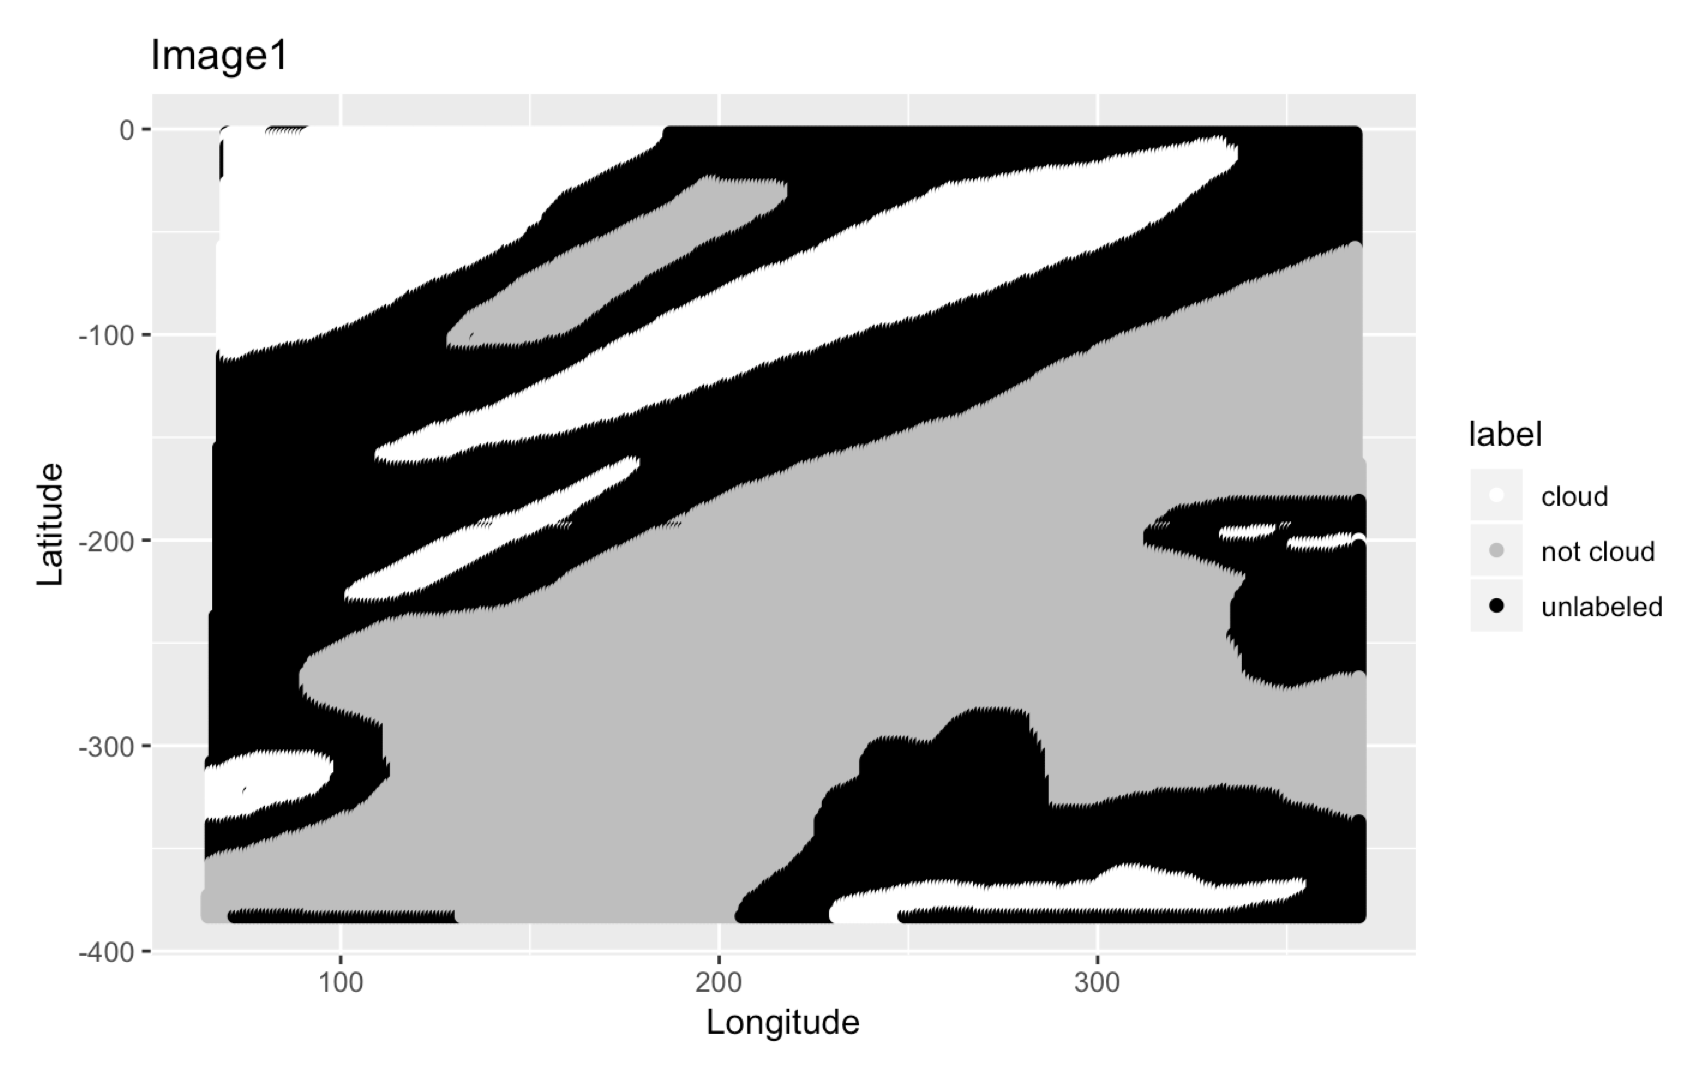
\includegraphics[width = 6cm]{1(b)image1.png}
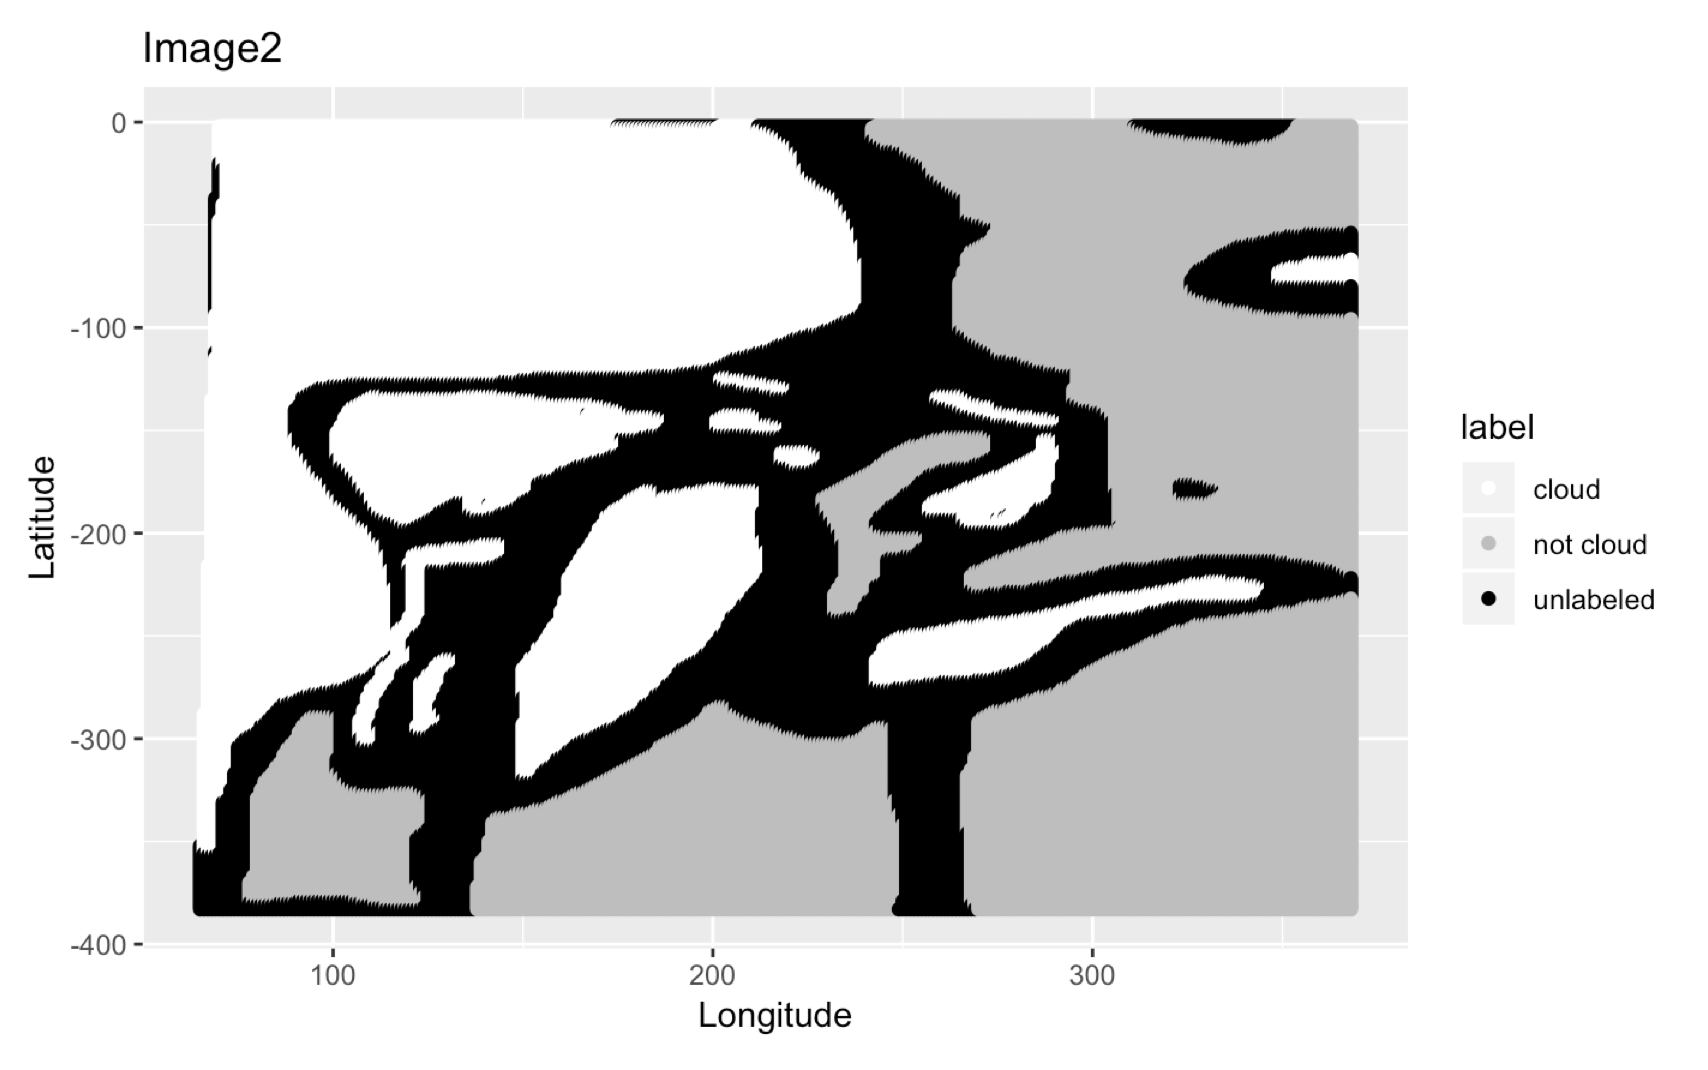
\includegraphics[width = 6cm]{1(b)image2.png}
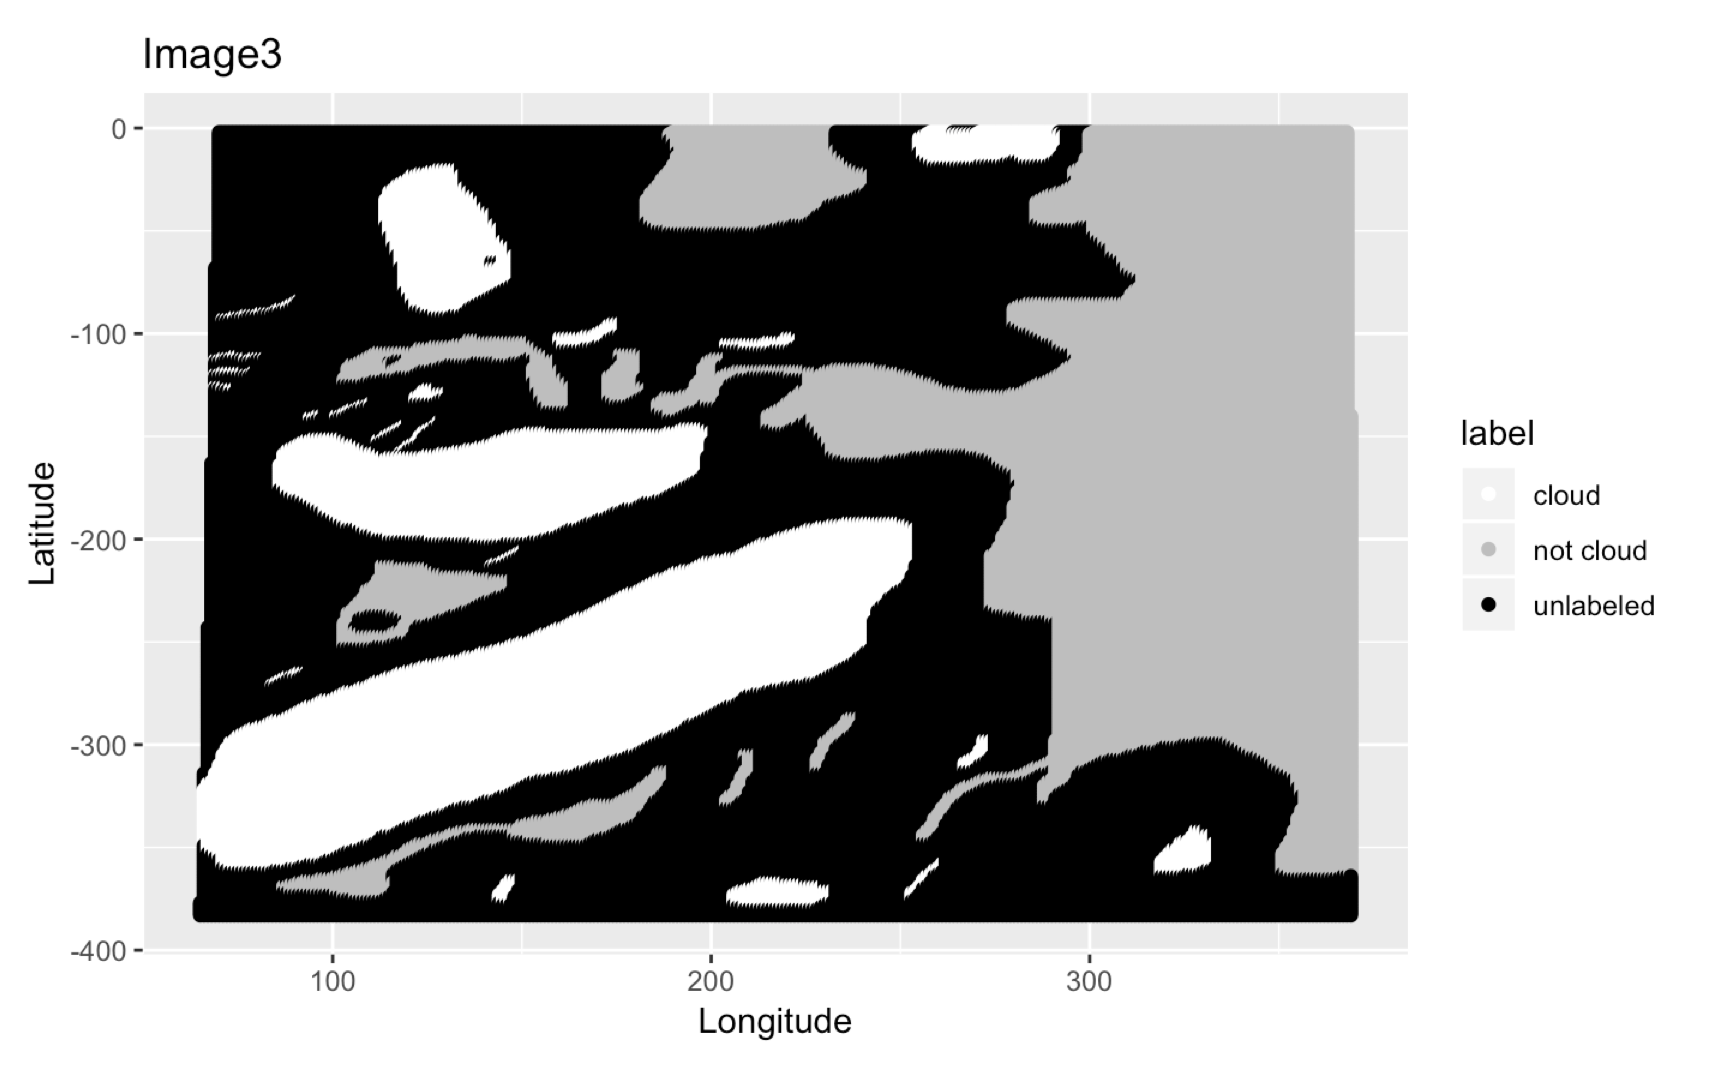
\includegraphics[width = 6cm]{1(b)image3.png}

From the three plots, we can see the pattern that the pixels with same labels are connected to each other, and unmarked pixels stay around those marked as clouds. This pattern contradicts to our assumption that the samples are i.i.d., because the pixels adjcent to pixels marked as clouds are more likely to be marked as clouds.


\vspace{0.3cm}
\mbox{}\\
\textbf{c. EDA}

To further explore our data, we also summarize the pairwise relationship between the features themselves.

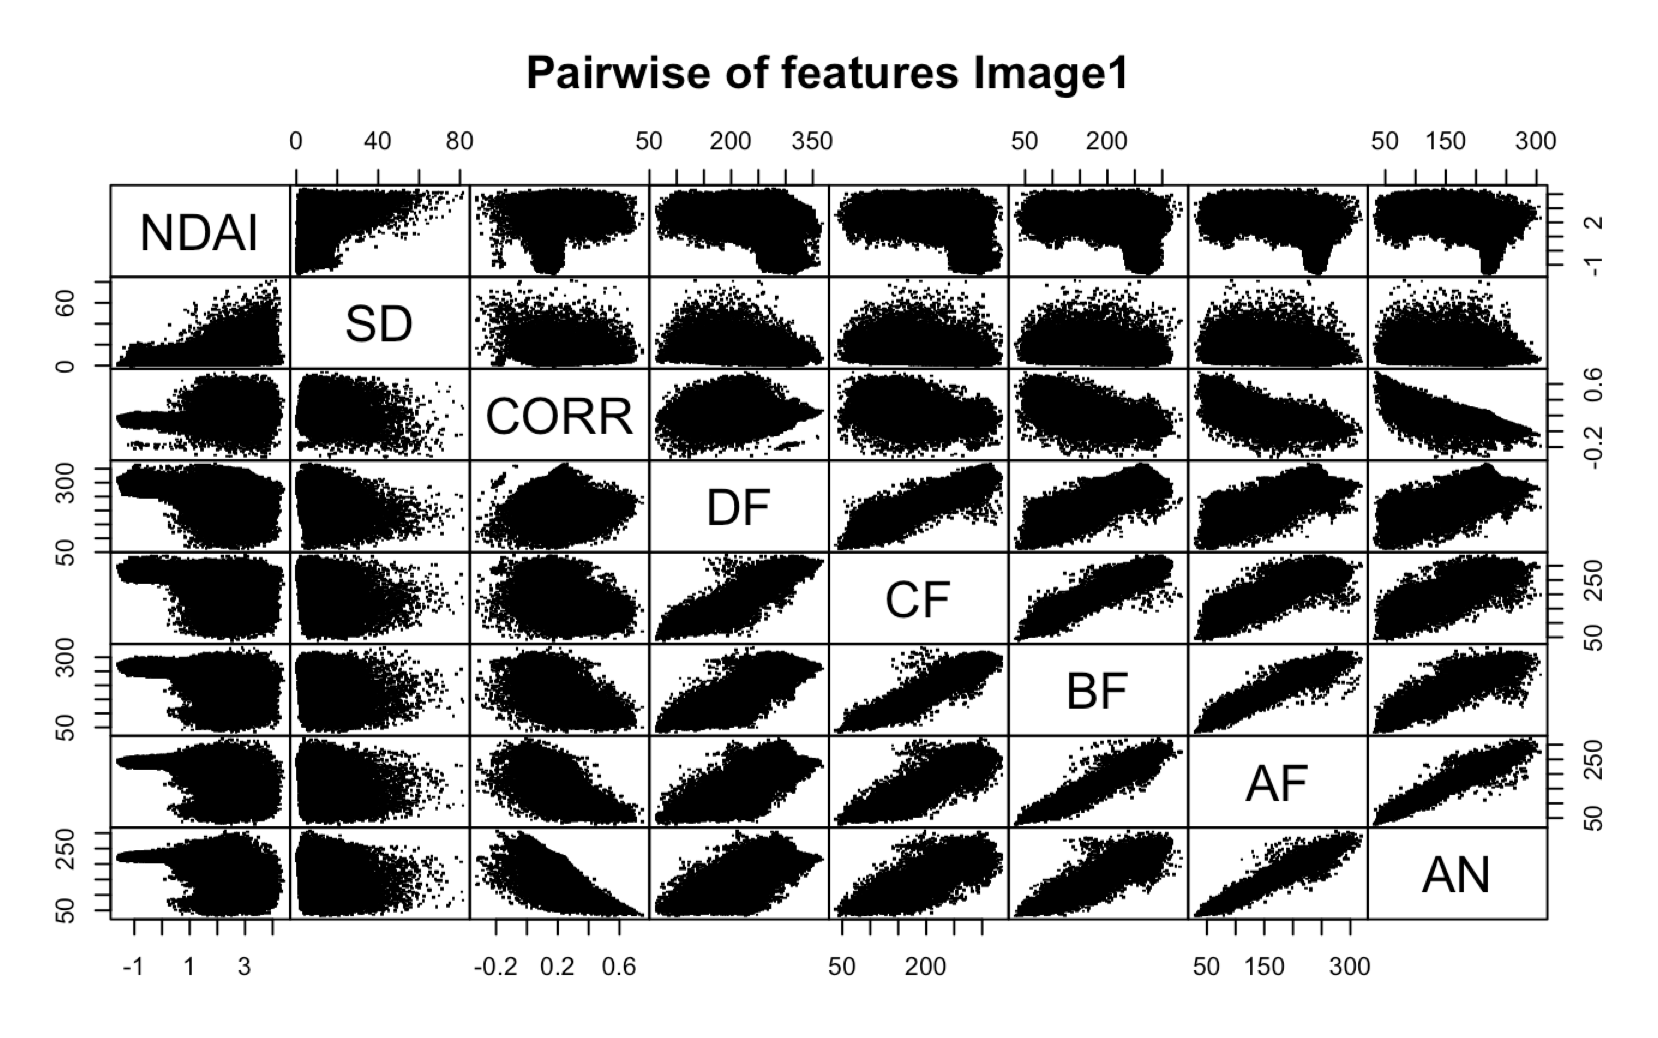
\includegraphics[width = 6cm]{1(c)image1.png}
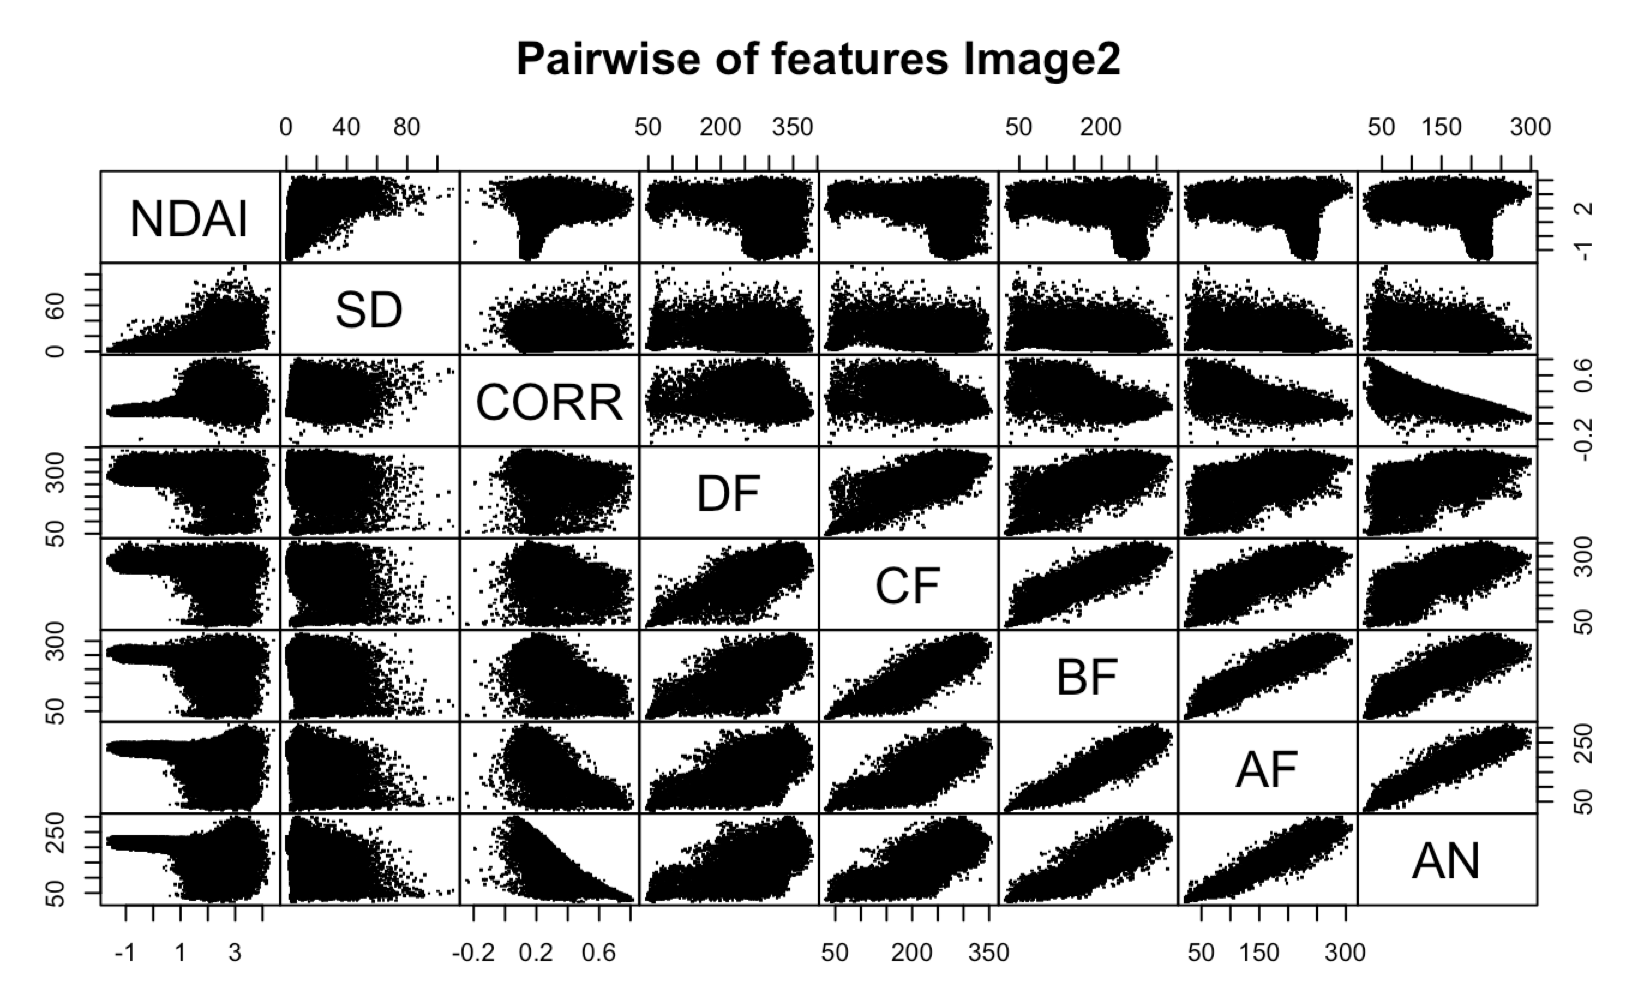
\includegraphics[width = 6cm]{1(c)image2.png}
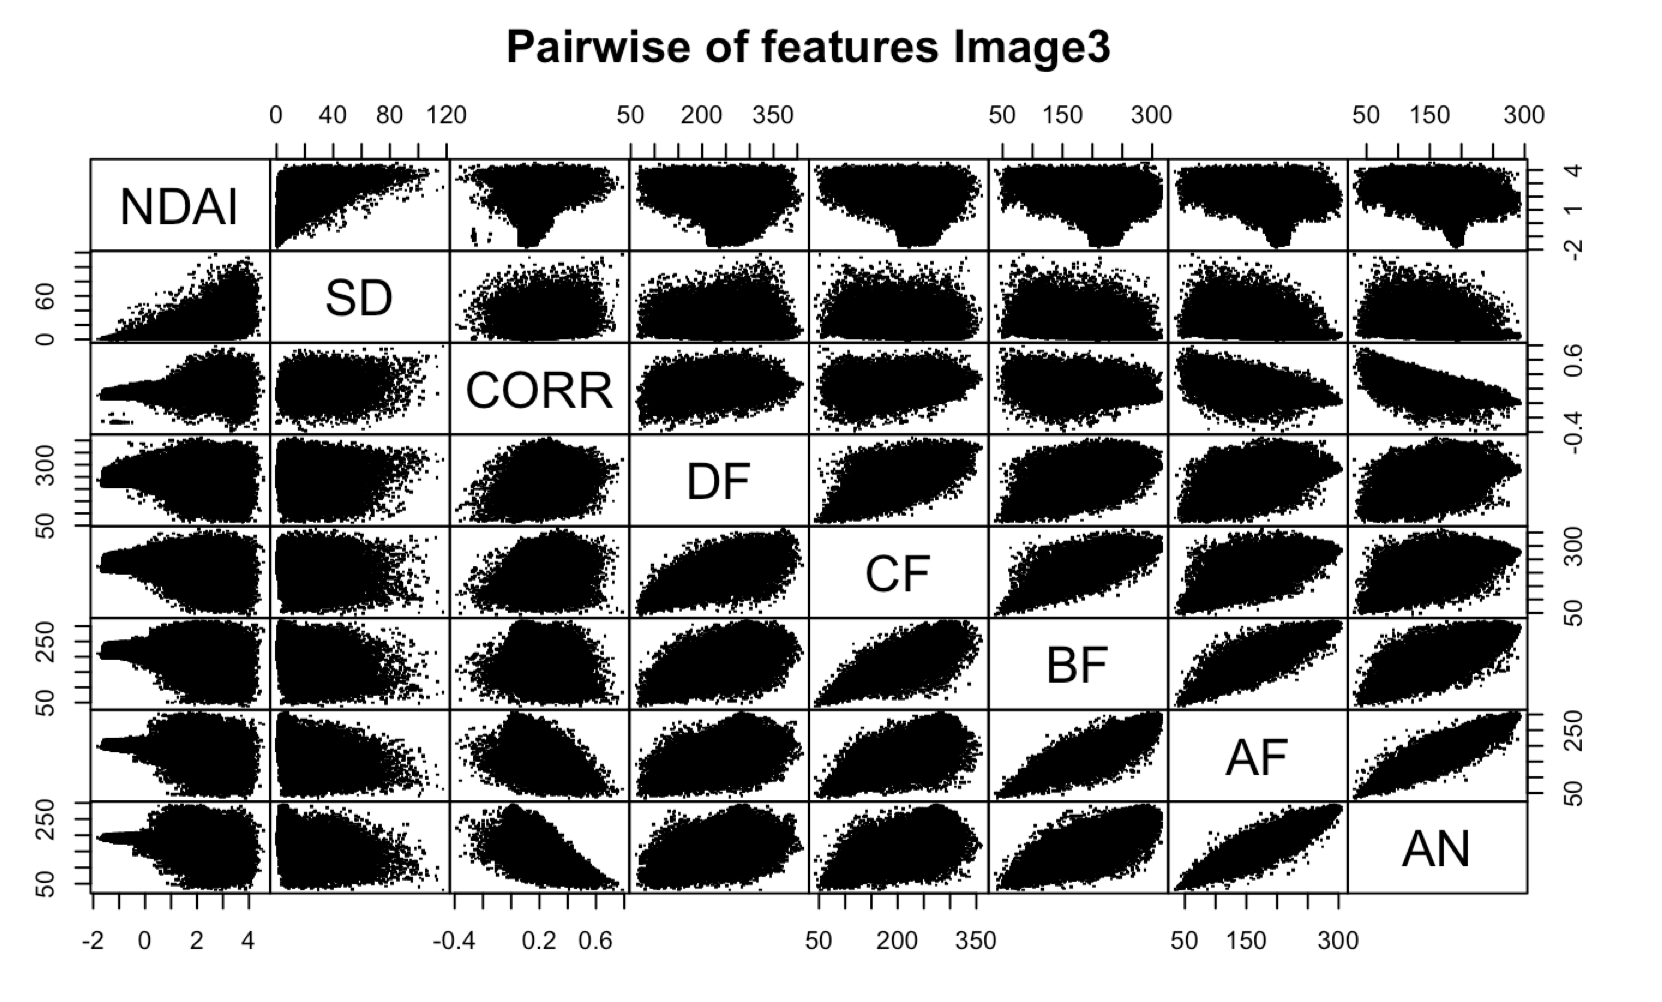
\includegraphics[width = 6cm]{1(c)image3.png}

The three pairwise scatterplots all show that DF, CF, BF, AF and AN shows a linear relationship between each other, especially for AF and AN, AF and BF. However, we observe that data points in the third pairwise scatterplot spread more widely than in the first two pairwise sctterplots. The differences between three graphs can also show that the (linear) relationships decrease over time.

After checking pairwise relationship plots, we study the relationship between each independent featues and their expert labels for each image and all data combined.

(relationship between expert label and NDAI)

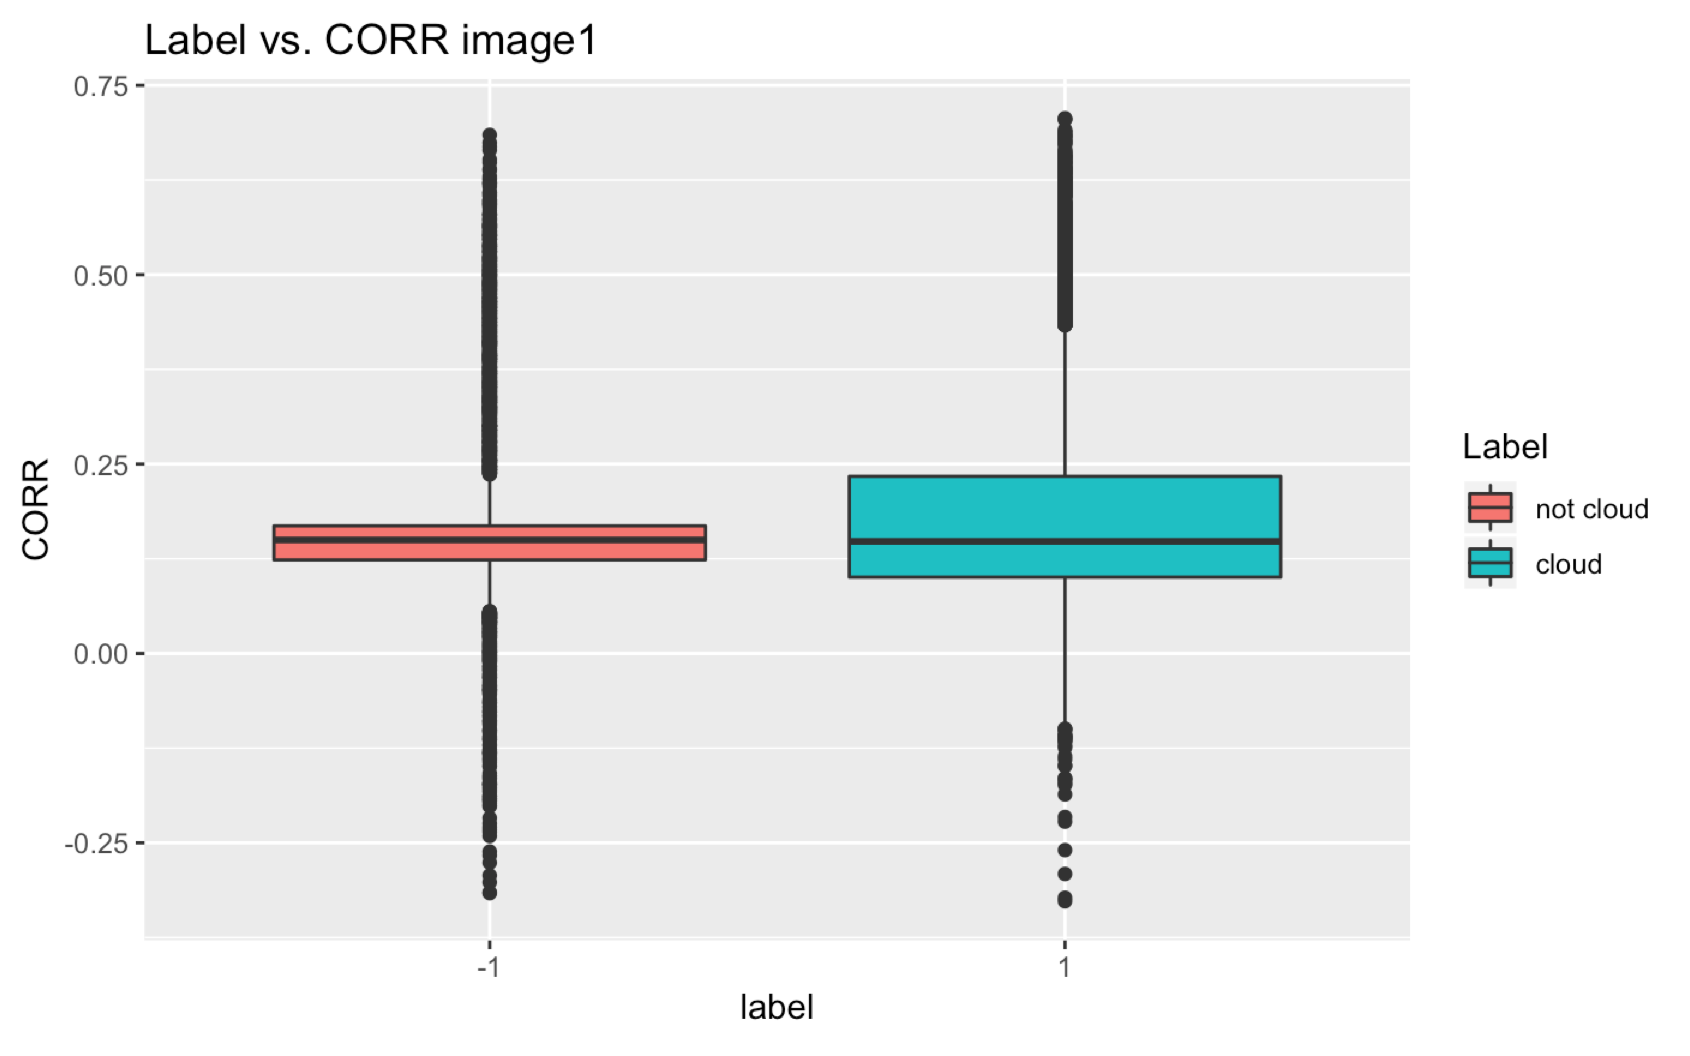
\includegraphics[width = 4.5cm]{1(c)image4.png}
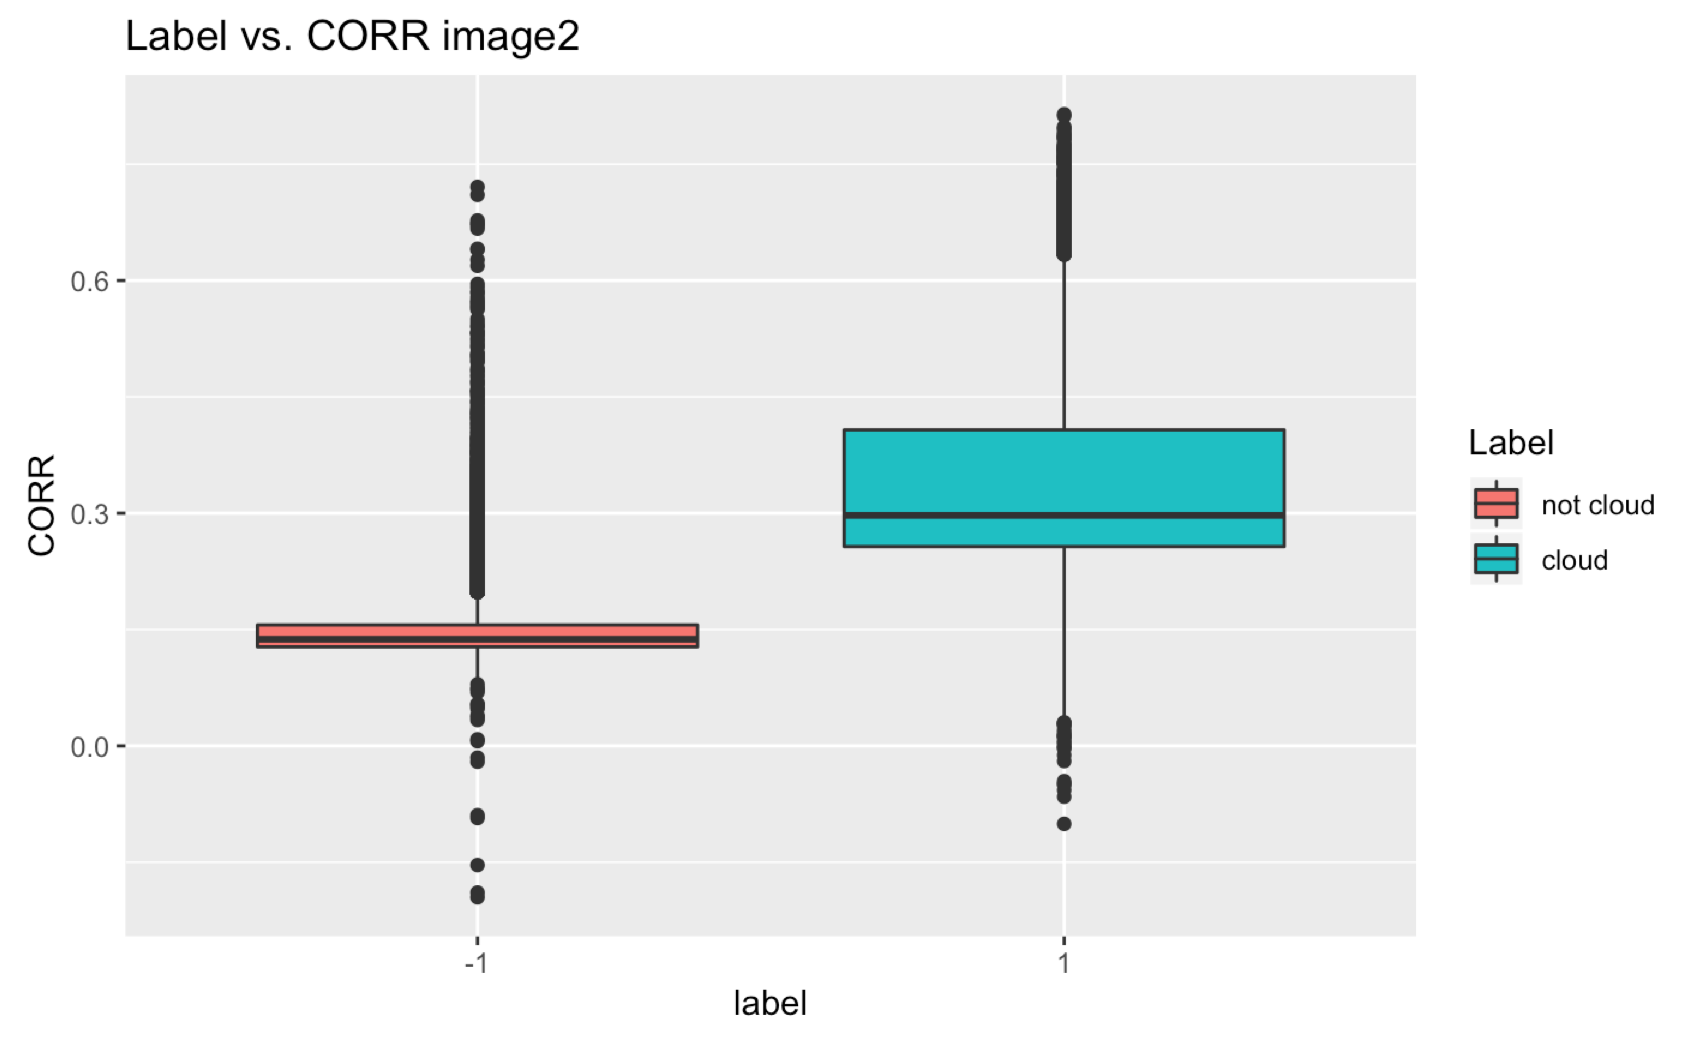
\includegraphics[width = 4.5cm]{1(c)image5.png}
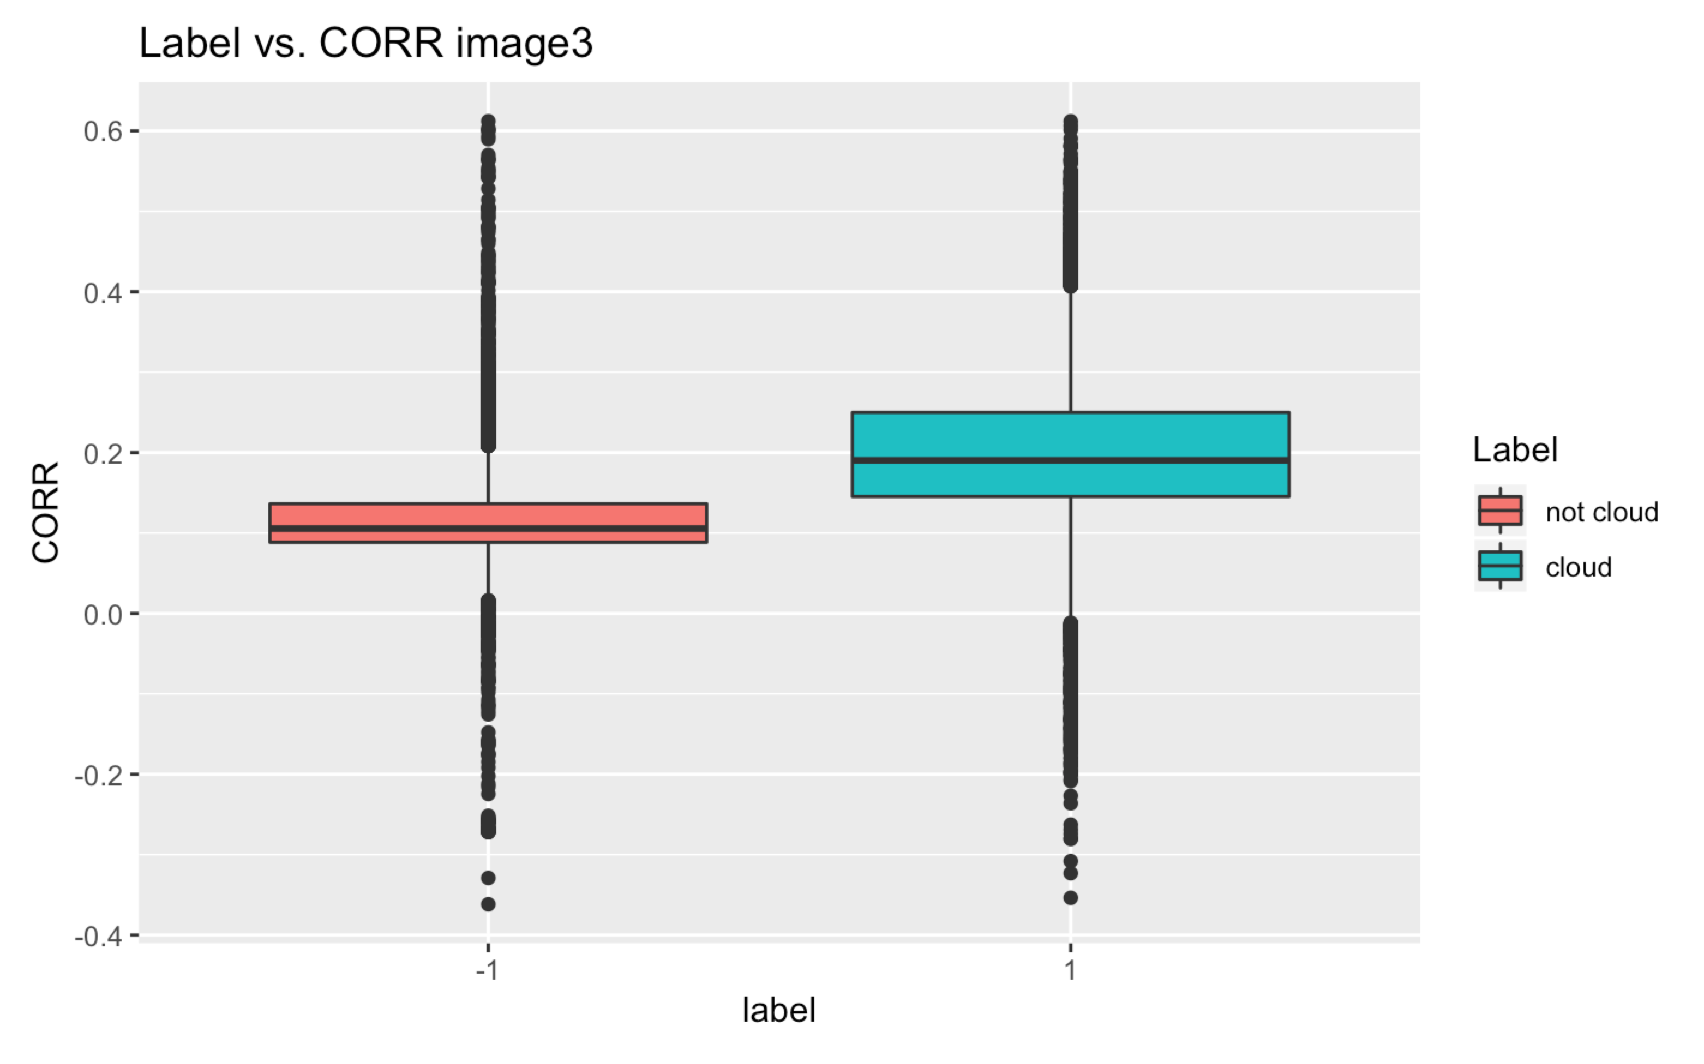
\includegraphics[width = 4.5cm]{1(c)image6.png}
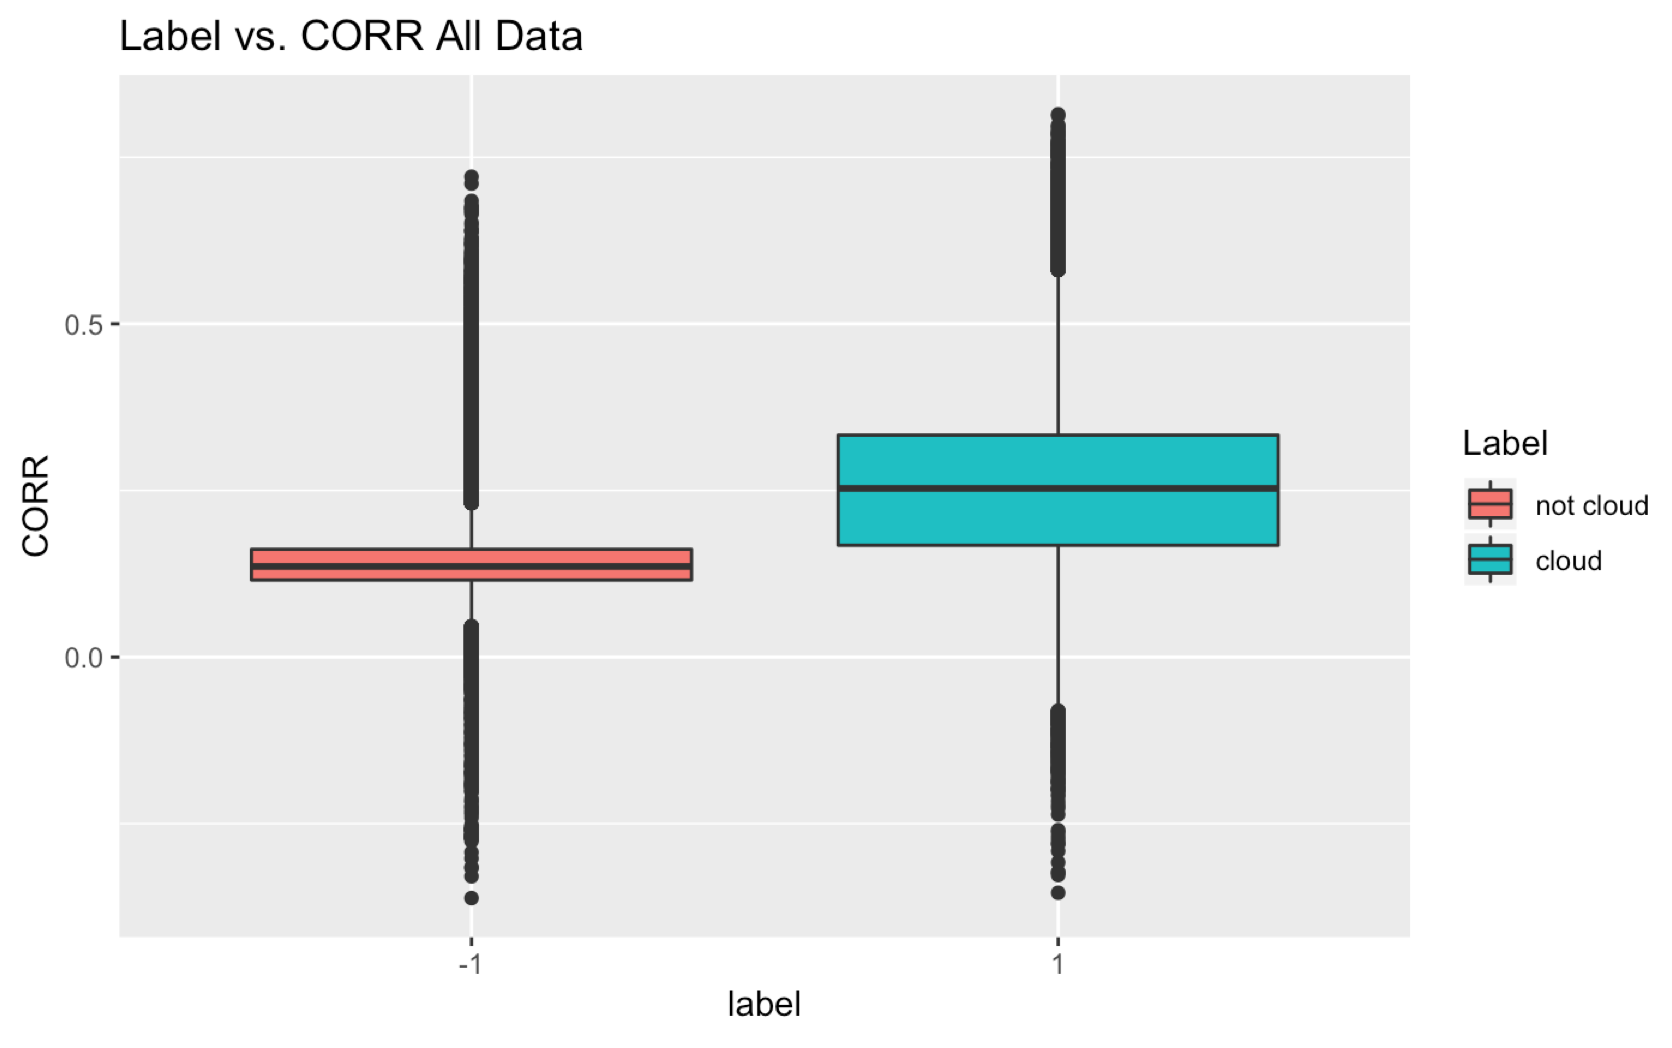
\includegraphics[width = 4.5cm]{1(c)image7.png}

The boxplots for CORR based on different labels show that CORR is on average higher for pixels marked as cloud than as not cloud. CORR also has a higher variance for those marked as cloud.

This conclusion contradicts to the statement in the paper that high correlations over cloud-free areas or low clouds are expected. This is because high correlations for clouds also occur under rare circumstances. More importantly, recklessly declare clear for high CORR pixels and cloudy for low CORR pixels will produce errors due to smoothness of surface terrain and the difference of attitudes of clouds.

Therefore, we should also involve the feature SD to identify surfaces into our investigation. We first plot SD vs. Label independently for each image and all data.

\mbox{}\\
(relationship between expert label and SD)

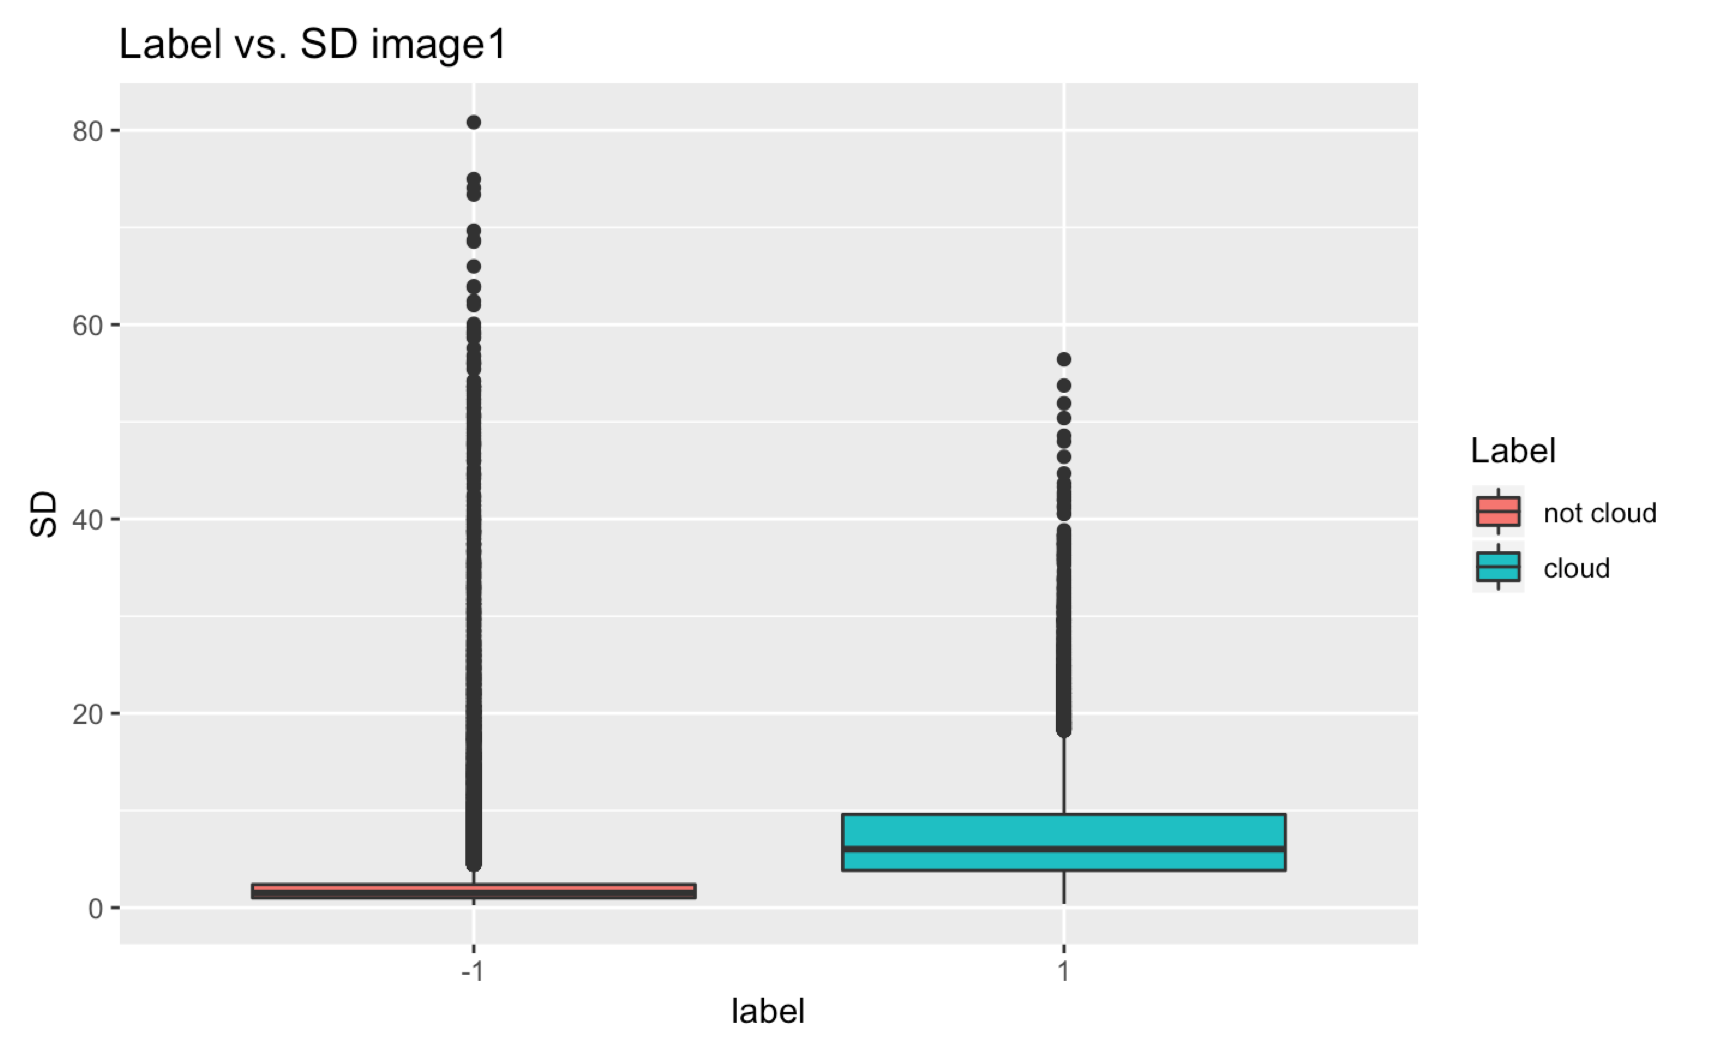
\includegraphics[width = 4.5cm]{1(c)image8.png}
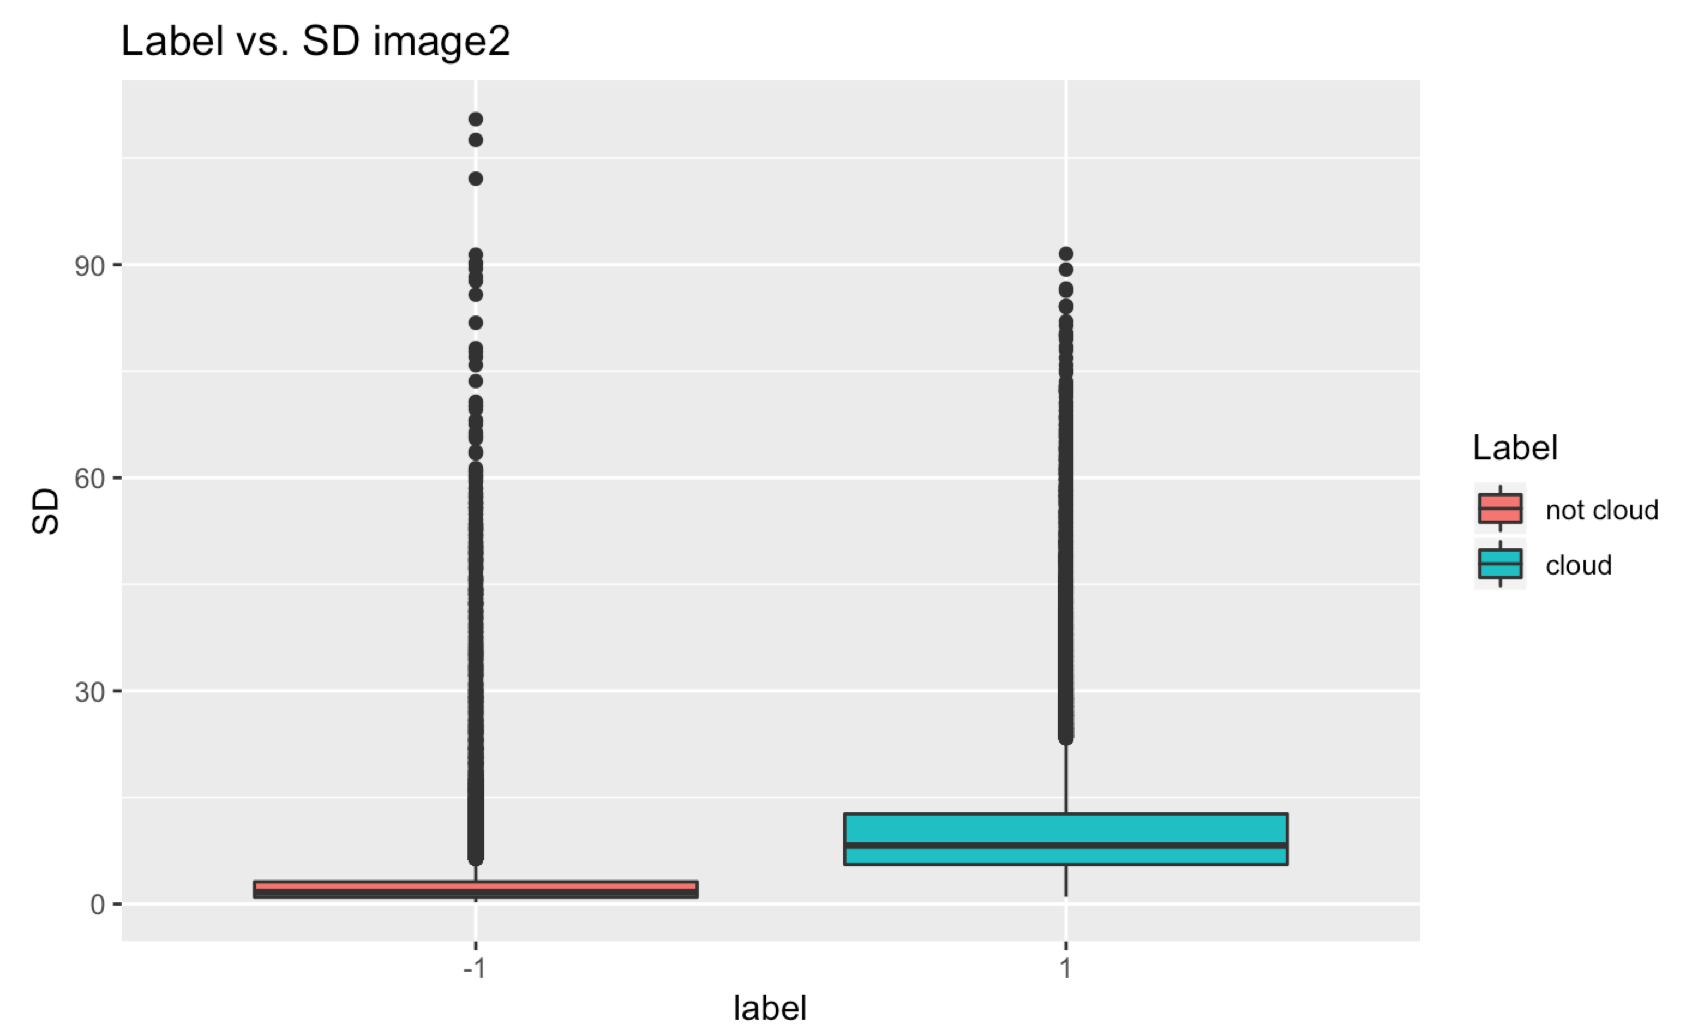
\includegraphics[width = 4.5cm]{1(c)image9.png}
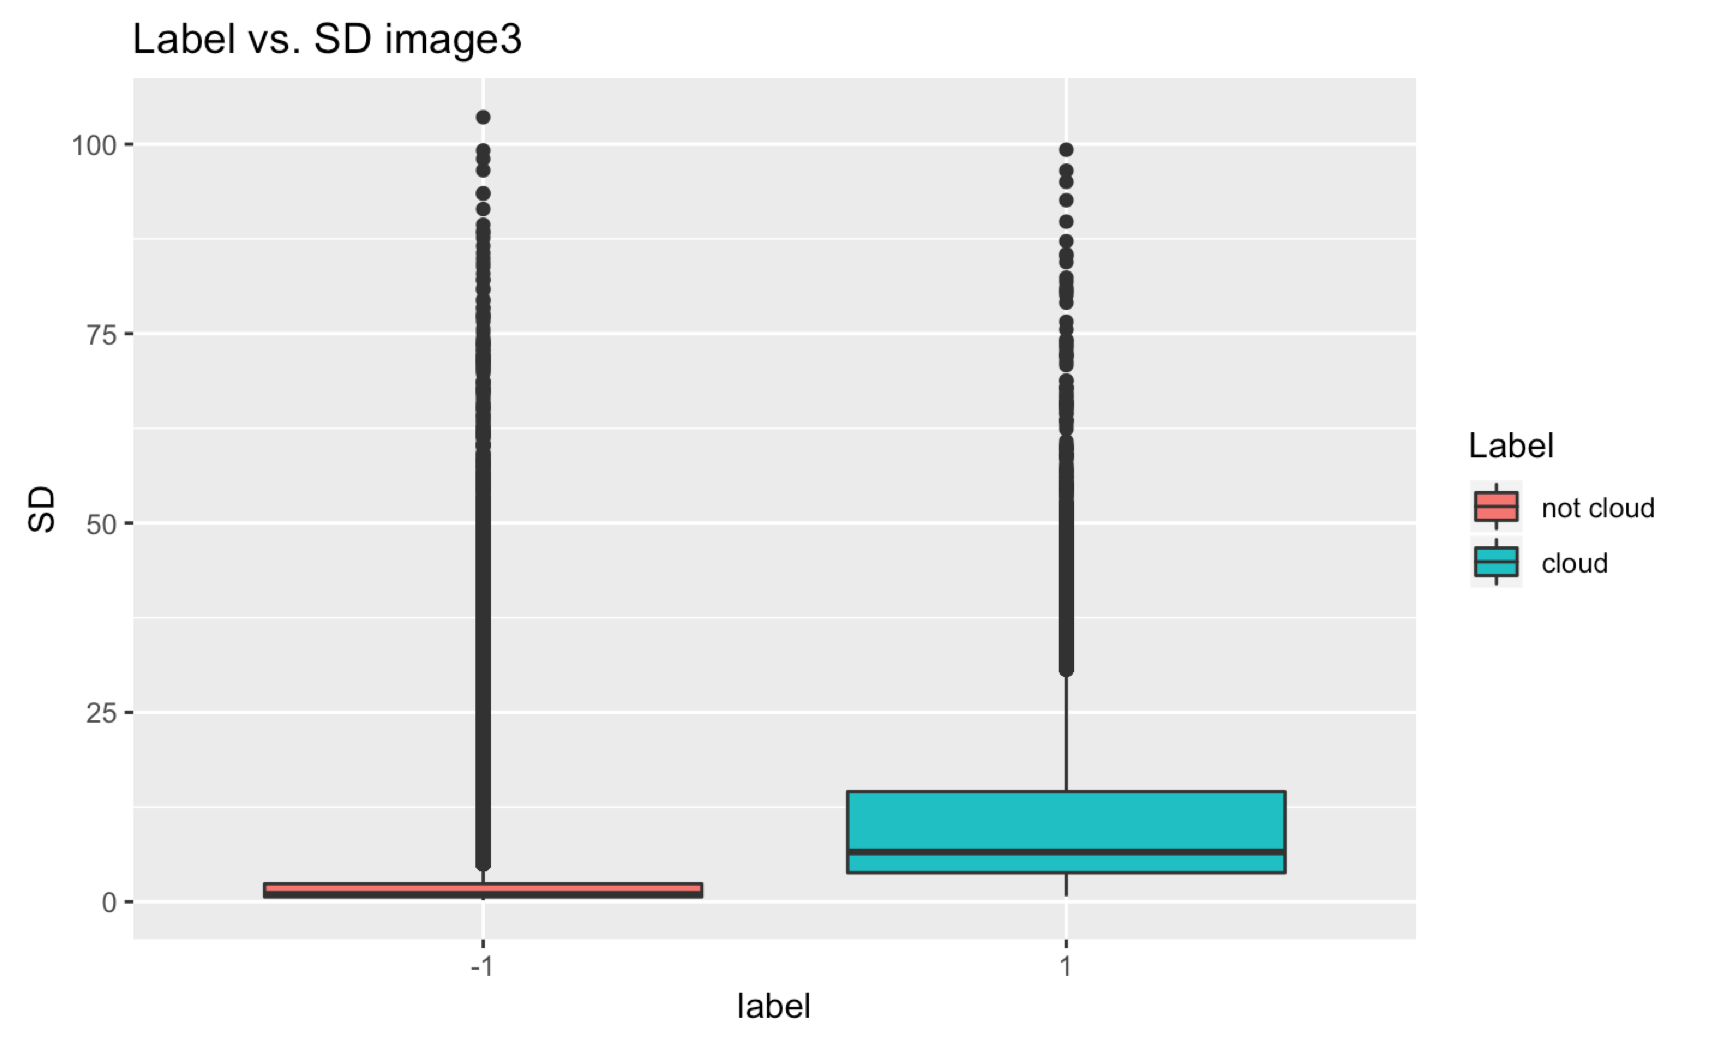
\includegraphics[width = 4.5cm]{1(c)image10.png}
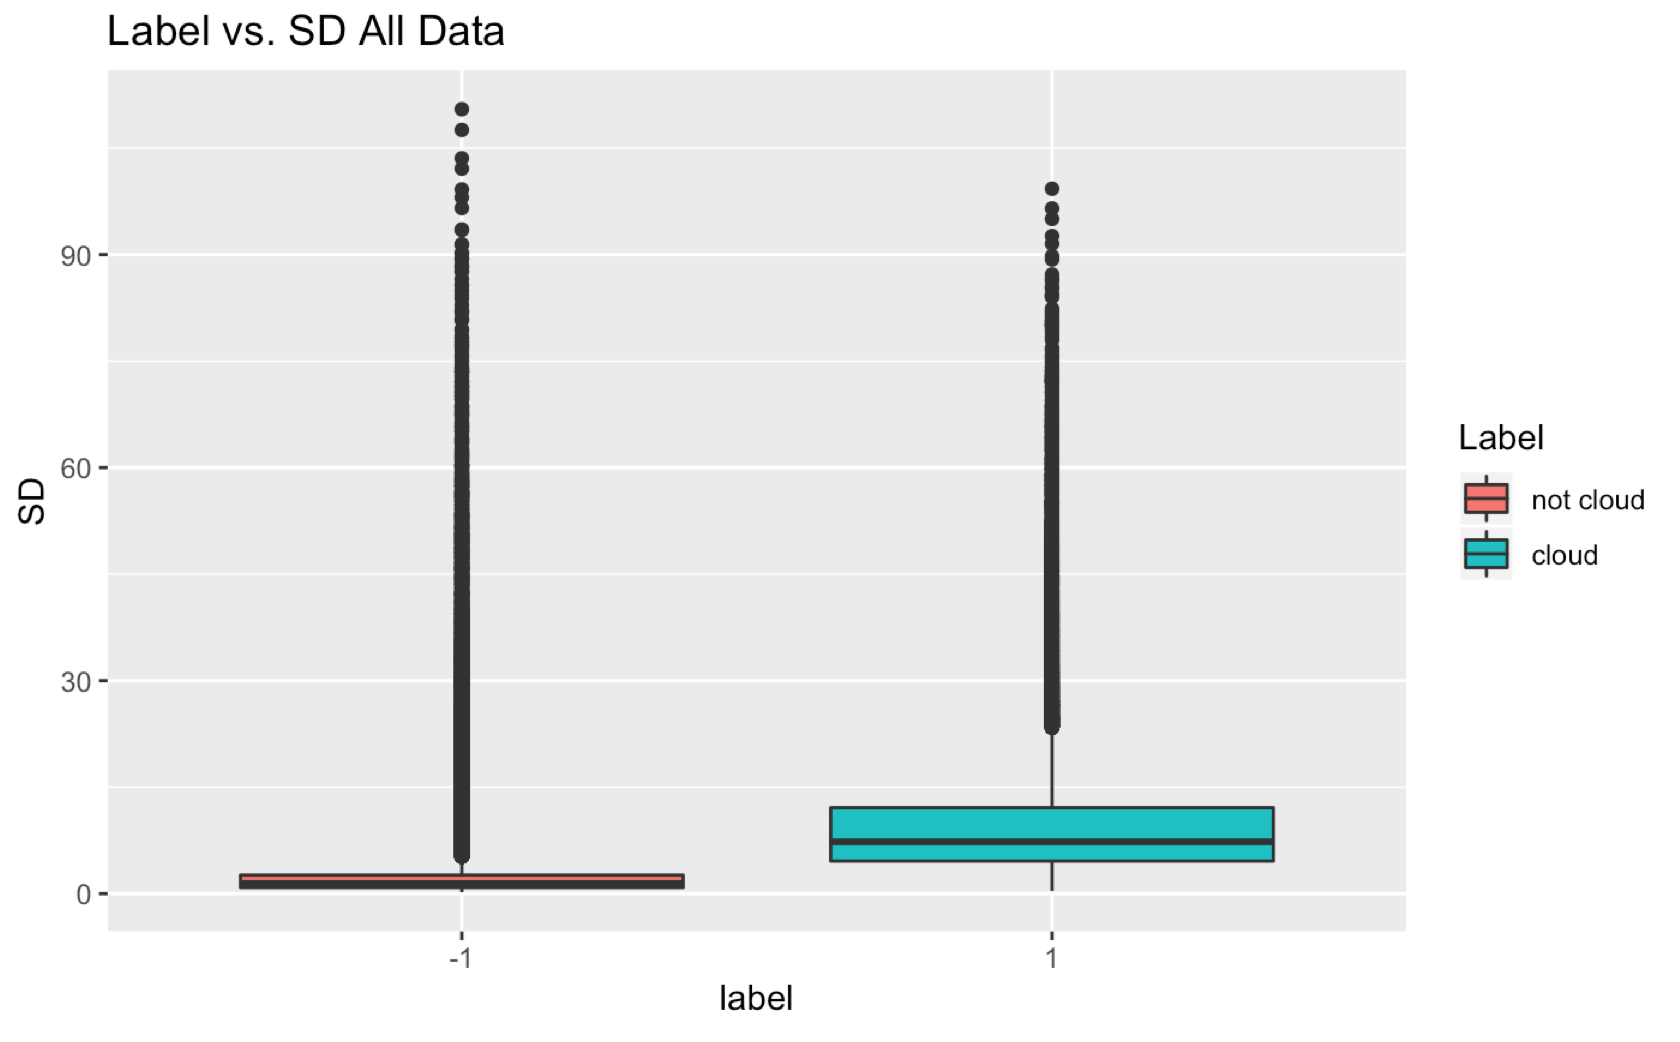
\includegraphics[width = 4.5cm]{1(c)image11.png}

From the boxplots for SD based on different labels, we can clearly see that the SD is higher for cloud pixels than those cloud-free ones. But the cloud-free pixels spread more widely. It can be explained that SD are usually small for radiation emanating from smooth surfaces.

Finally, the thrid feature NDAI relates to the differences for isoreopic level of surface-leaving radiation between low-attitude clouds and snow-coved surfaces.

\mbox{}\\
(relationship between expert label and NDAI)

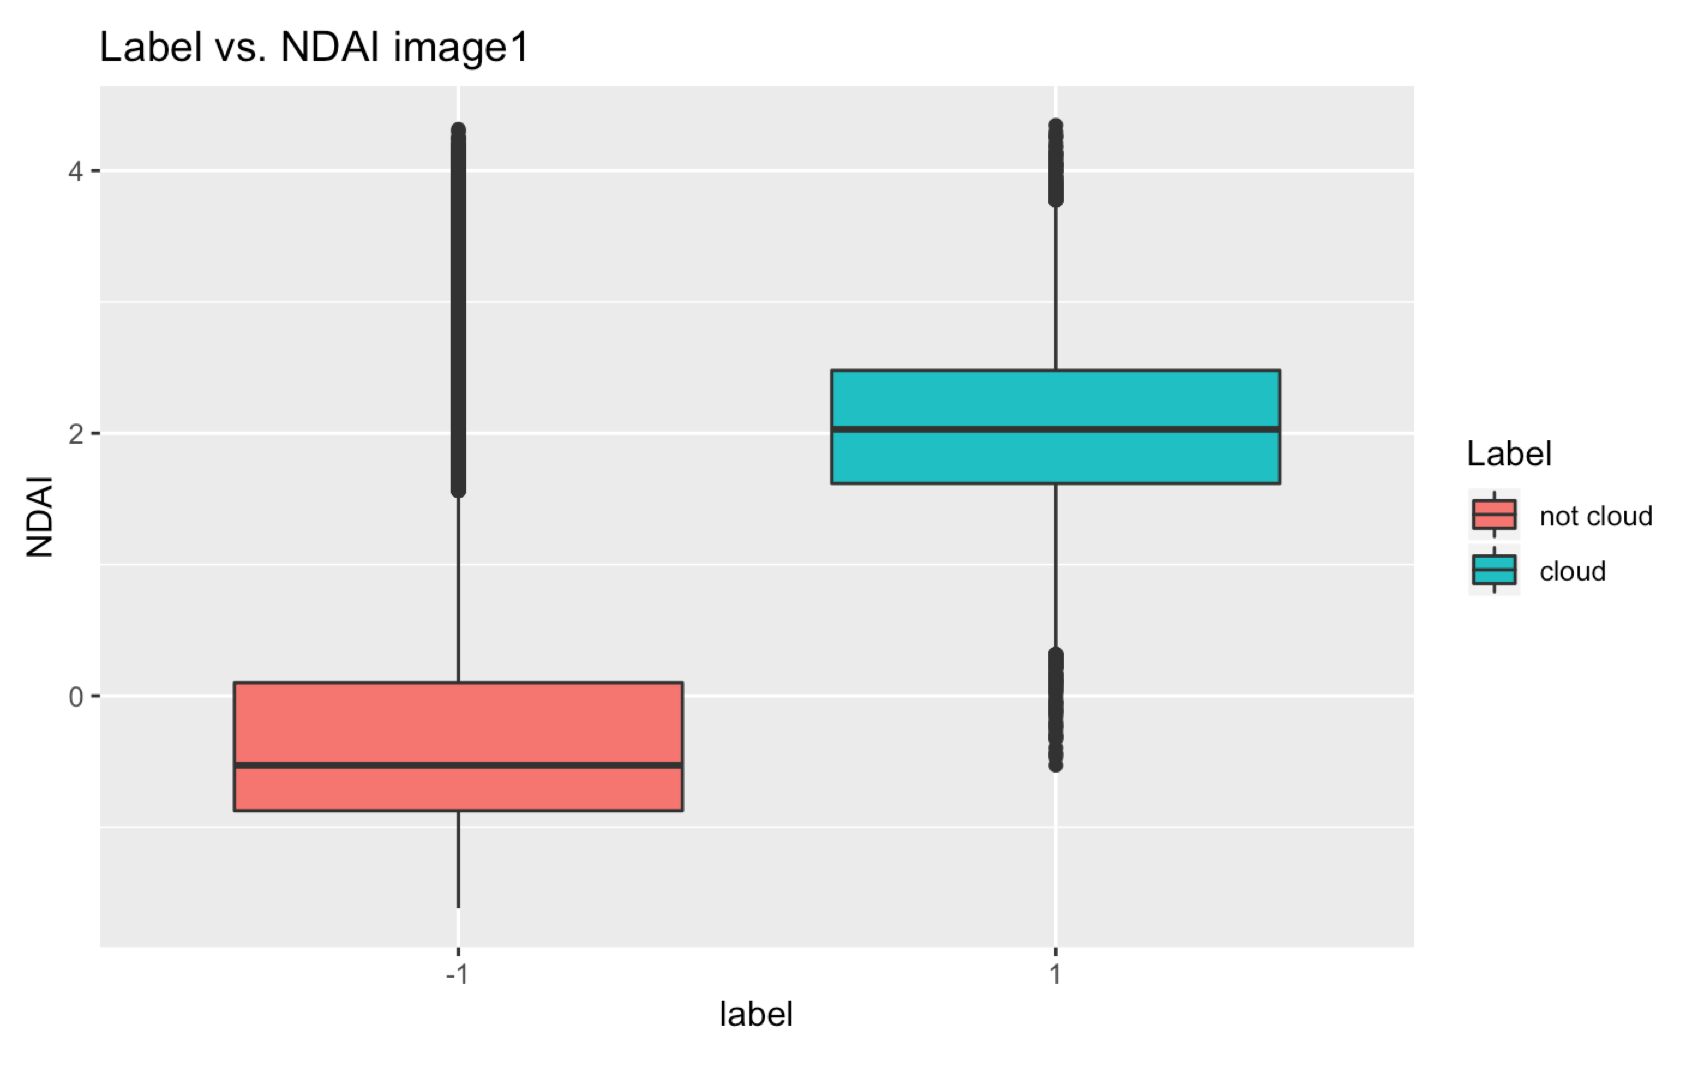
\includegraphics[width = 4.5cm]{1(c)image12.png}
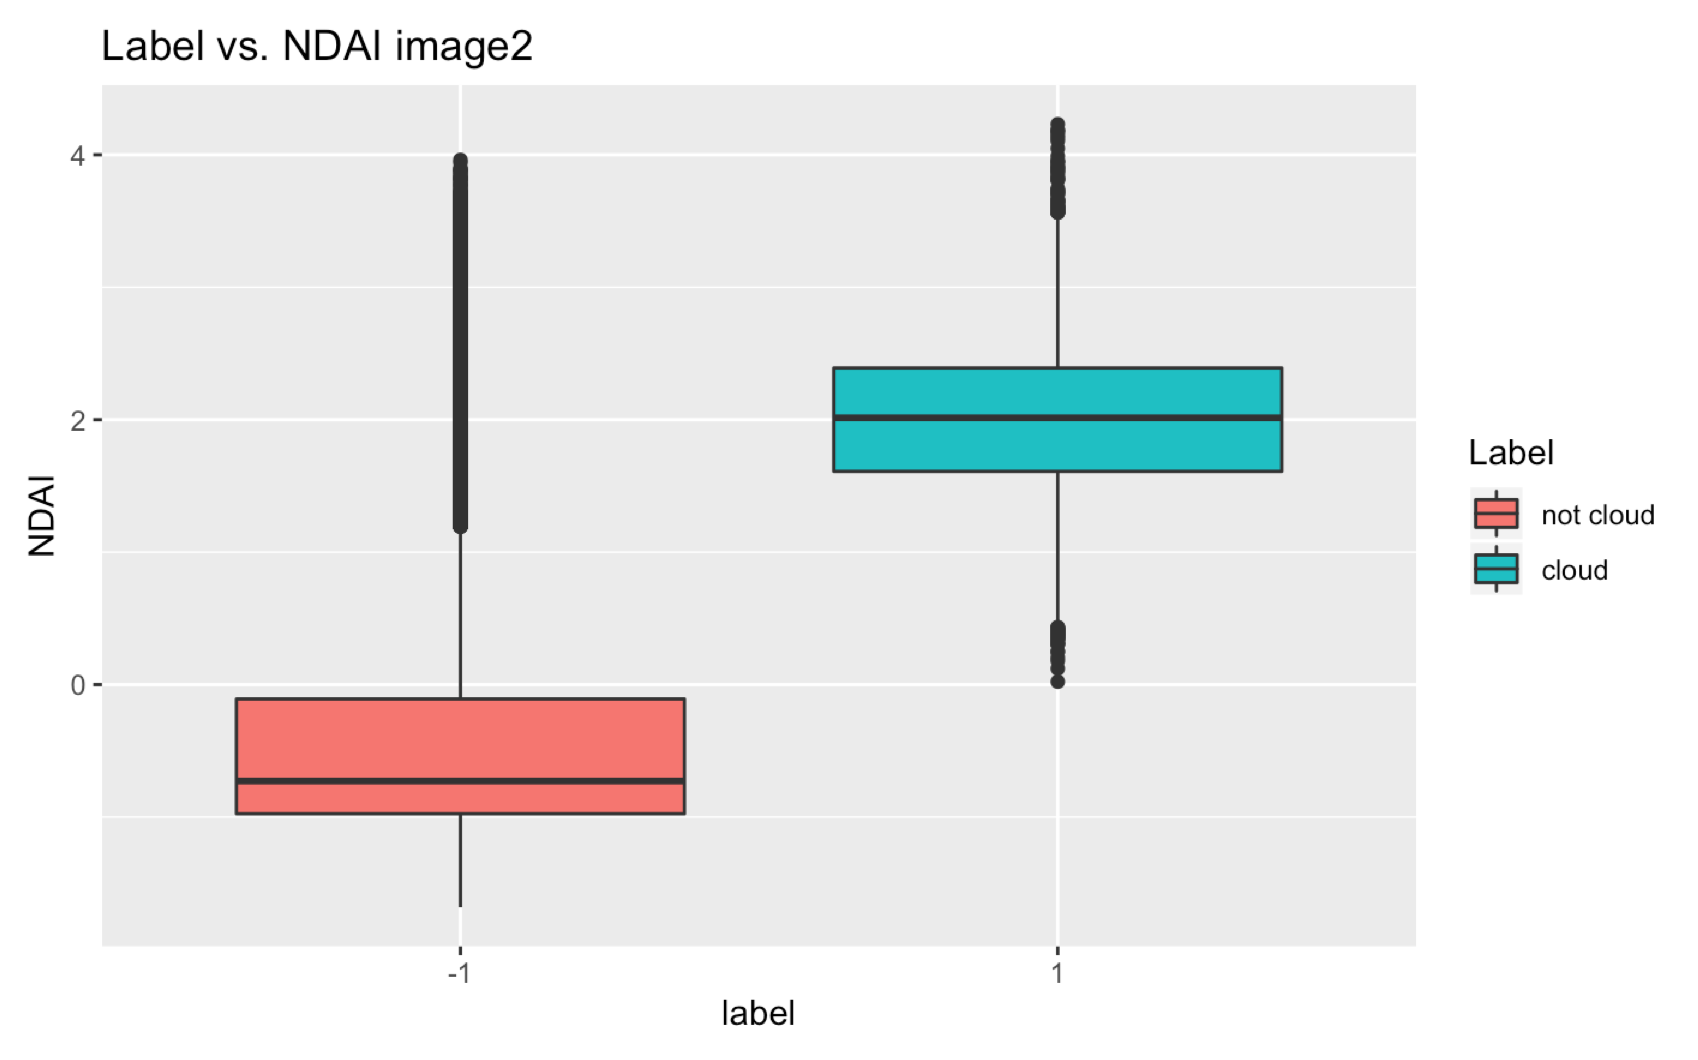
\includegraphics[width = 4.5cm]{1(c)image13.png}
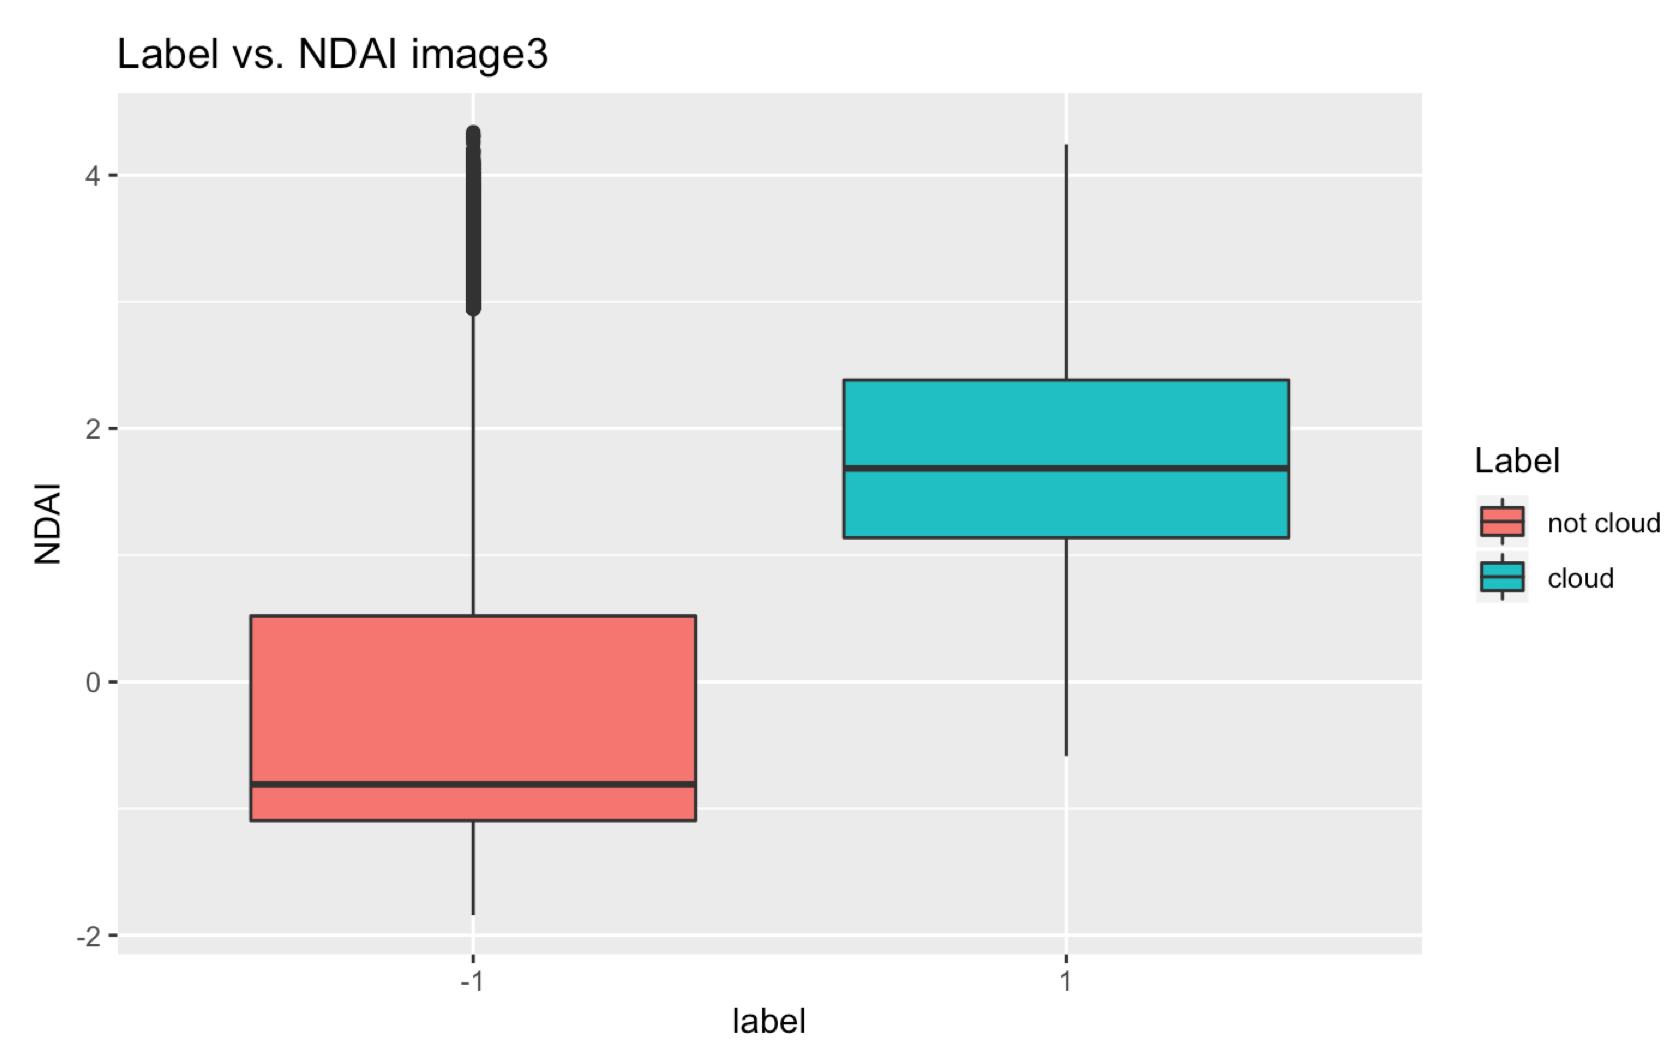
\includegraphics[width = 4.5cm]{1(c)image14.png}
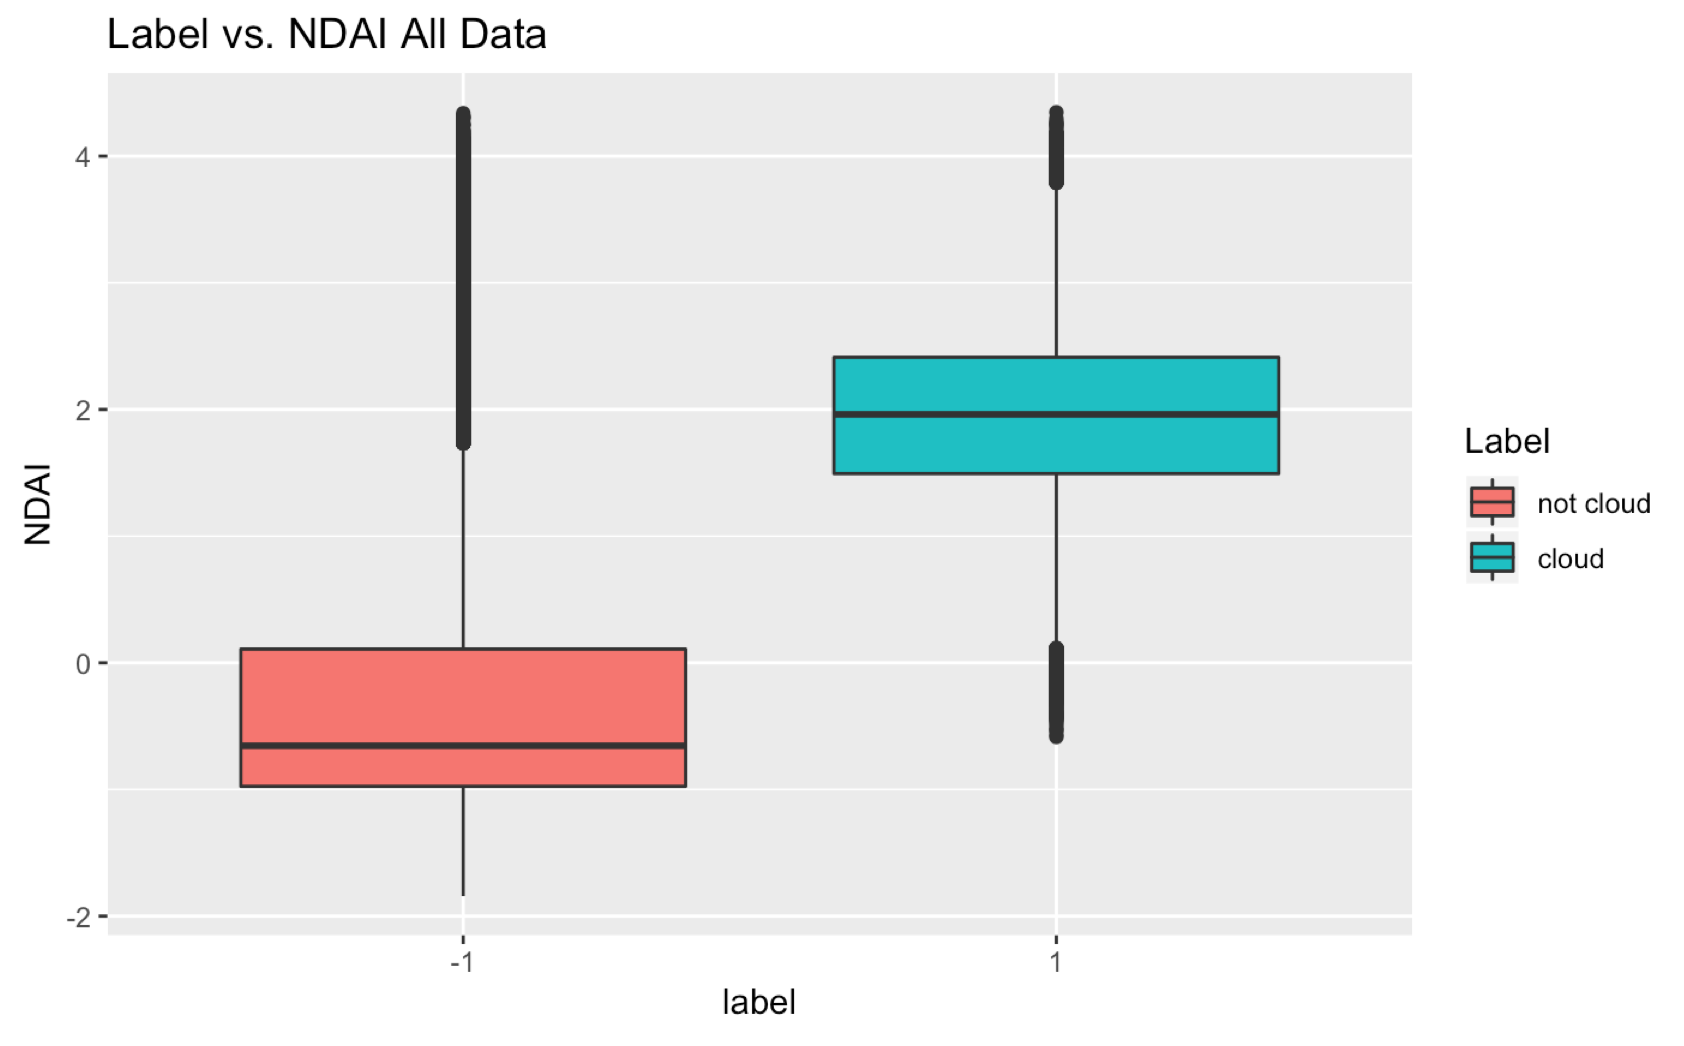
\includegraphics[width = 4.5cm]{1(c)image15.png}

From the boxplots for NDAI based on different labels, we can clearly see that the NDAI is higher for cloud pixels than those cloud-free ones. The distrubition for cloud-free pixels are left skewed, while the distribution for pixels marked as cloud are roughly symmetric. The distribution for three different image data are roughly the same as well.

\section{Preparation}

\vspace{0.2cm}
\textbf{a. Data Split}

Even though the three image data set represent the cloud dsitribution at different times at the same place, we still decide to combine the data into one to have more data for training. We also clear out the unlabeled data here because they are not helpful enough for classification problem. Since the data are not i.i.d., we cannot simply split the data by random. 

First method:
We decided to divide the data into 25 groups by cutting the image horizontally. In this case, data with y\_coord from 2.0-78.2 and the corresponding x-coordinate are in the same group.  We randomly select 23 groups from these 25 groups as training/validation data and 2 groups as test data. In the 23 groups, we randomly sampled 18 groups as validation data. Splitting the data in this way looks like a one-stage cluster sampling. Every time we sample a group wihout replacement and include all data points in that group. Data in the same groups tend to be correlated to each other, which fit the property of the non i.i.d. data.

Our Second method is, for each image data set, to divide all the data into 25 groups by cutting the image into 5*5 small images. For instance, data with y\_coord from 2.0-78.2 and x\_coord from 65.0-125.8 are in the same group. We randomly select 23 groups from these 25 groups as training/validation data and 2 groups as test data. In the 23 groups, we randomly sampled 18 groups as validation data. Splitting the data in this way looks like stratified sampling. Every time we sample a group wihout replacement and include all data points in that group. We can also see this method as combining small pixels into a much larger one in a visual way. This method can guarantee pixels that have high correlations (adjacent pixels) can be sampled at the same time (except those on the boundary). And the random sampling on the 25 groups can make sure that we are not too sticking to the patterns for the training data so that overfitting can be somewhat prevented. 

\vspace{0.3cm}
\mbox{}\\
\textbf{b. Baseline}

Setting all labels to -1, the accuracy for test data is 0.520 and that for validation data is 0.270, which are relatively low. If the test data and validation data contain mostly -1, the trivial classifier will have a high average accuracy.

\vspace{0.3cm}
\mbox{}\\
\textbf{c. First Order Importance}

Recall in the EDA part, we notice that five raw features(DF, CF, BF, AF, AN) have high linear relationship between each other. To have more information represented by features, we will choose at most one from these five features.

To find three best features, we first caculate and plot the correlation between those features and the expert labels. The magnitudes of the absolute values of the correlations represent how close the relationships are between features and expert labels. Larger correlation value means better features. We found that NDAI and CORR are better than others on average. 

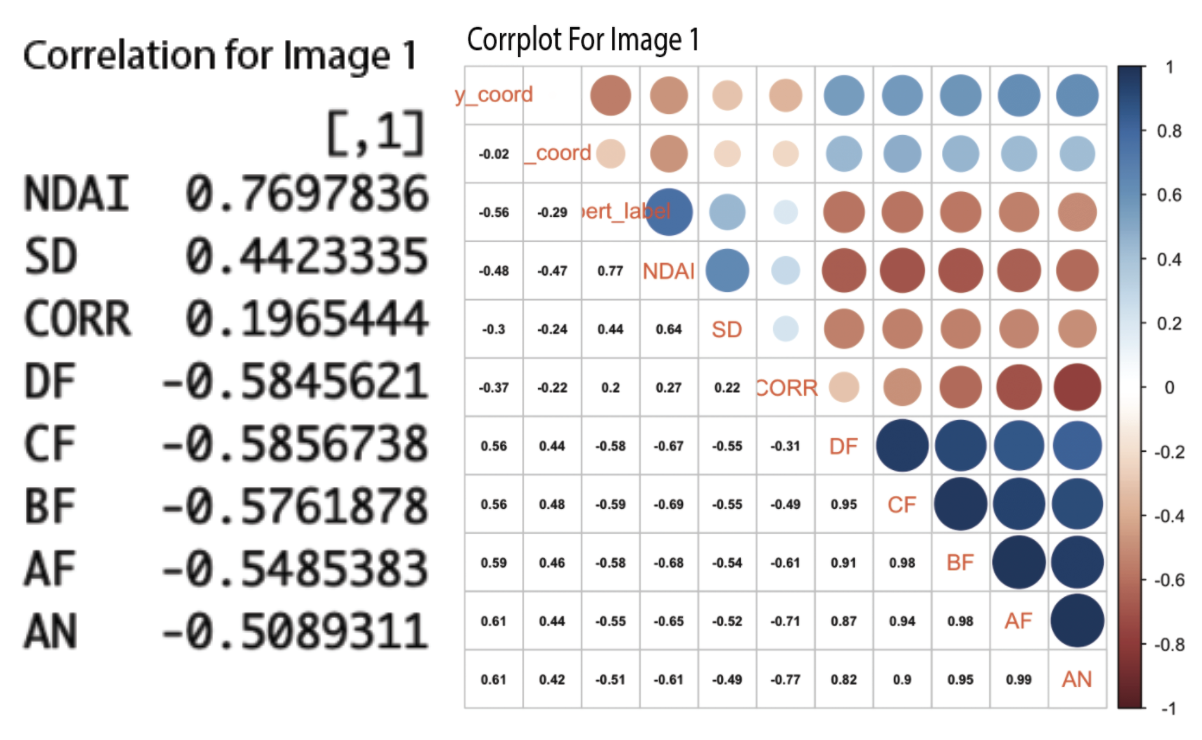
\includegraphics[width = 5.5cm]{2(c)image1.png}
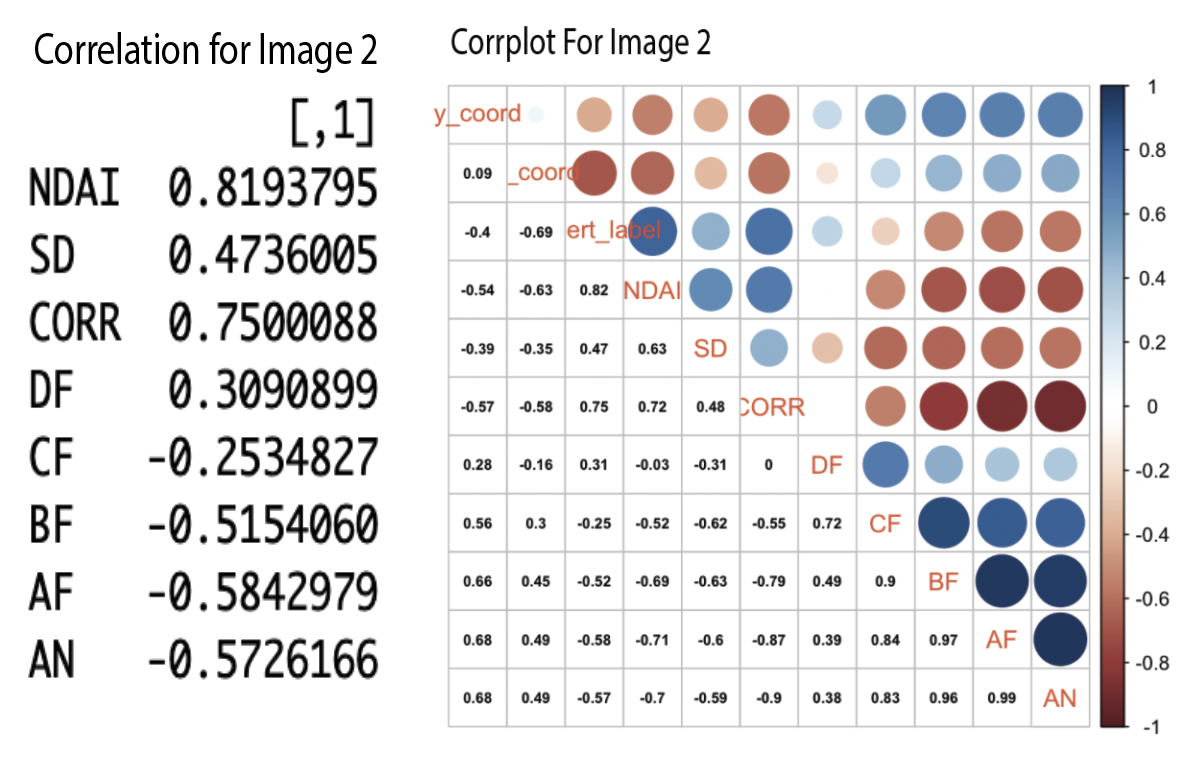
\includegraphics[width = 5.5cm]{2(c)image2.png}
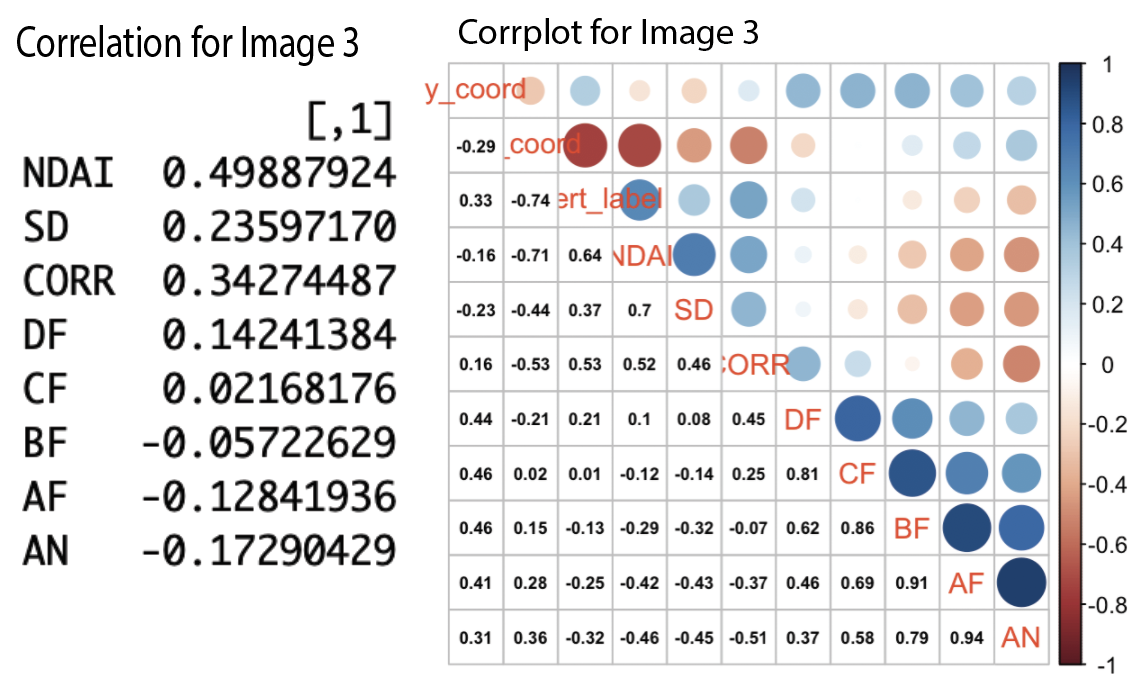
\includegraphics[width = 5.5cm]{2(c)image3.png}

Then, we plot biplots and loadings on first two PCs to see how much each feature contributes to these PCs. We choose to use two PCs because they capture almost 90\% of the data which is enough to represent the entire data set. The loading plots can illustrate the association between features and PCs. The larger the loading of a feature in a given PC, the more associated the feature is with that PC. After viewing the four loading plots, we observe that SD and DF have larger loadings than other features (expect NDAI and CORR). Considering there are other reasons that is more associated with scientific explanation, we decide to be consistent with the three features chosen in the paper, which are CORR, NDAI and SD.


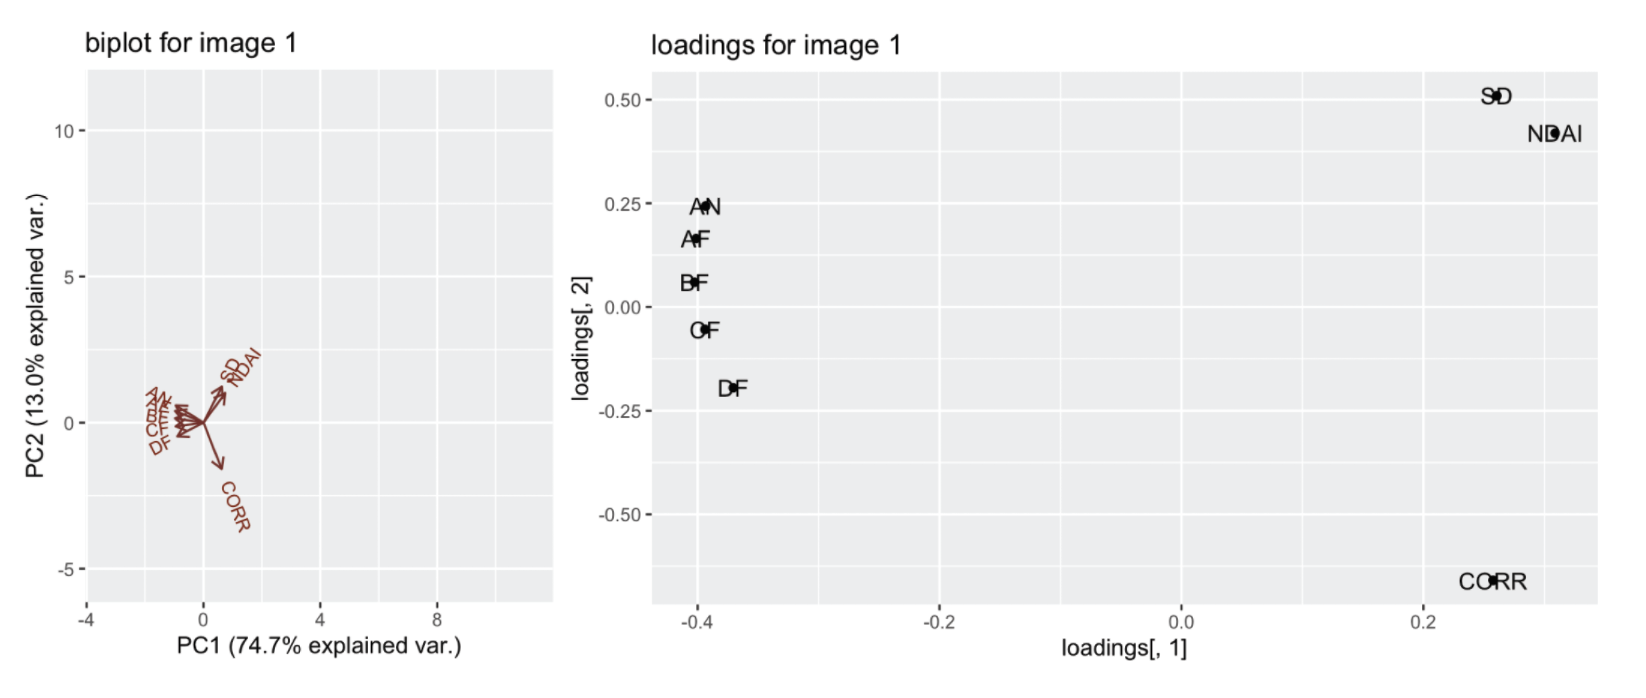
\includegraphics[width = 13cm]{2(c)pca1.png}

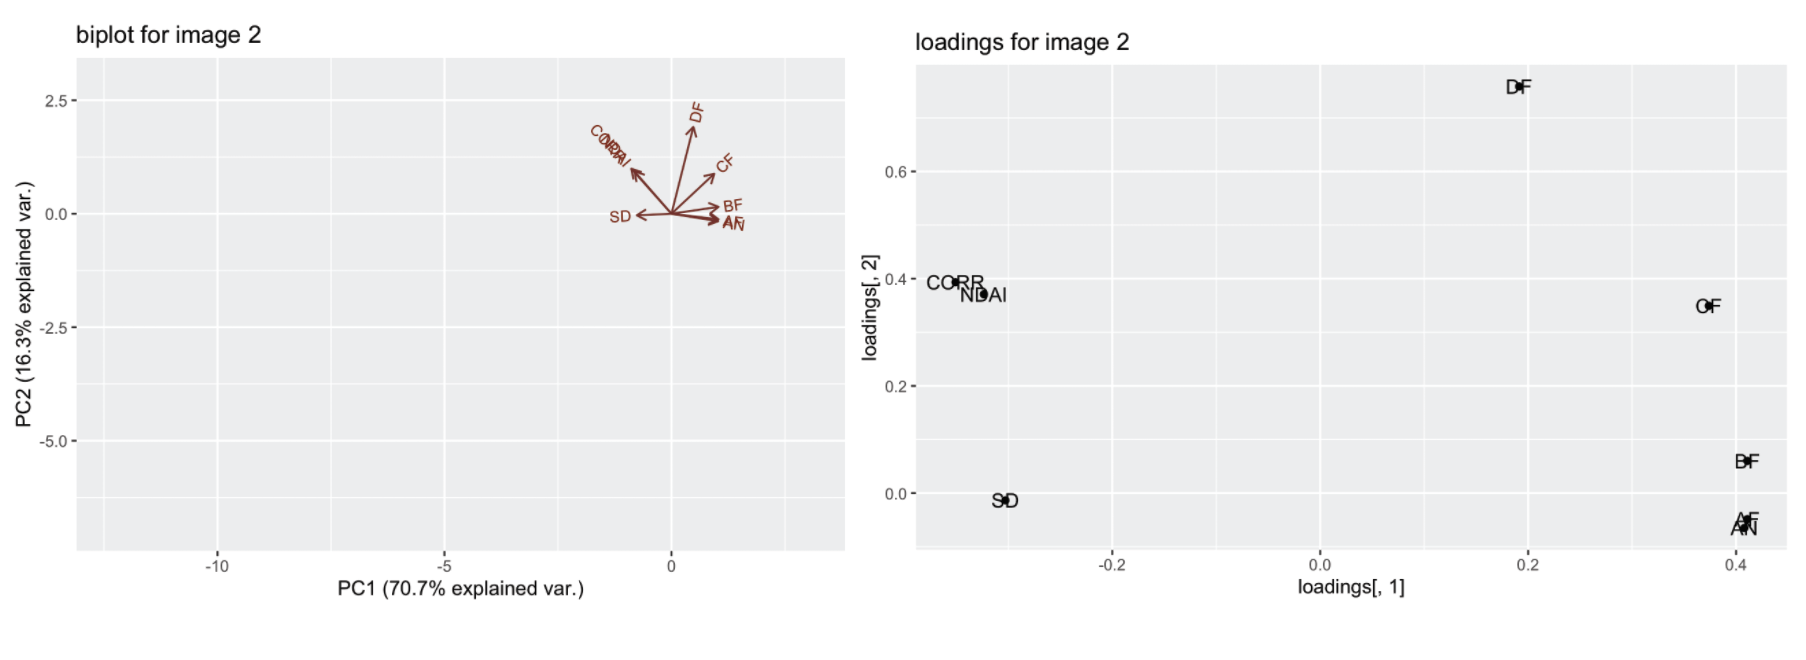
\includegraphics[width = 13cm]{2(c)pca2.png}

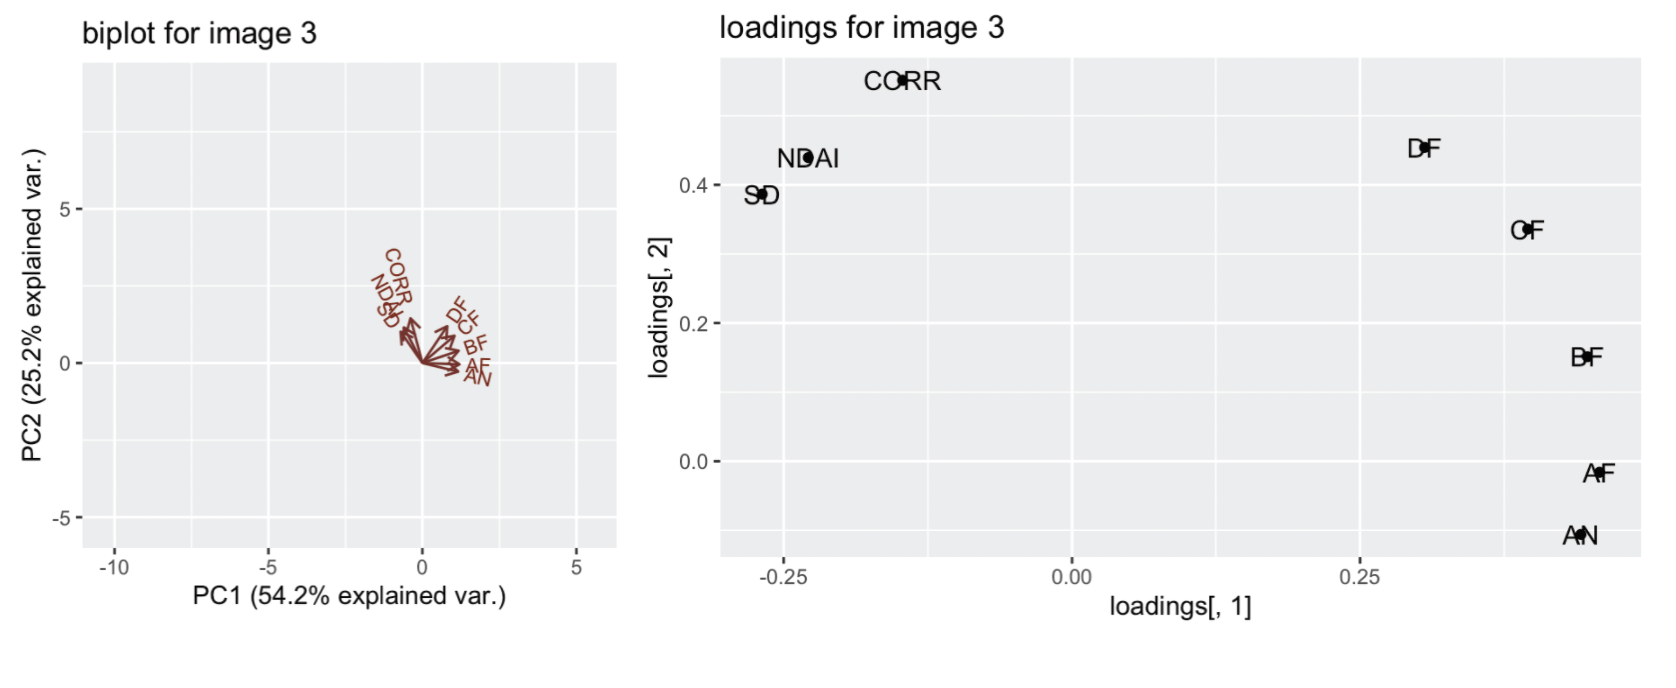
\includegraphics[width = 13cm]{2(c)pca3.png}

\vspace{0.3cm}
\mbox{}\\
\textbf{d. CVgeneric Function}

See \url{https://github.com/WinnieGao/Project2_Git} for more detailed explanation and code.



\section{Modeling}

\vspace{0.2cm}
\textbf{a. Different Classification Models}

To train the data, we try several different classification methods: Generalized Linear Model, Linear Discriminant Analysis, Quadratic Discriminant Analysis, K-nearest Neighbor and Support Vector Machine.
For GLM, LDA and QDA, since, in our natural world, most phenomena can be approximated using Gaussion distribution, we assume our data sets are under Gaussian distribution, which means LDA and QDA are applicable. Since Gaussian distribution is exponential family, we can also apply GLM in our case. Since there is no specific assumptions for using KNN and SVM, they are also satisfied.

We used cross-validation with 8 folds to train the models, and get the accuracies across all folds and the averaged one. We also apply the model on the test set and get the accuracy on the test set.

For our first splitting method, the cross-validataion average accuracies shows that LDA, QDA,SVM and KNN all return  great performance with an accuracy above 0.91. Among them, LDA performs the best on the validataion data with 0.9286555 accauray and GLM gives the lowest average cross-validation accuarcy. As for the performance on the test set, all models gives lower accurary about 0.7 to 0.8. KNN gives the best accuracy and GLM returns the worst performance on the test set. Considering both the accuracies on the validation and test set, QDA performs relatively better than other models. Hence, we conclude that QDA is the best model for the first spliting data.  

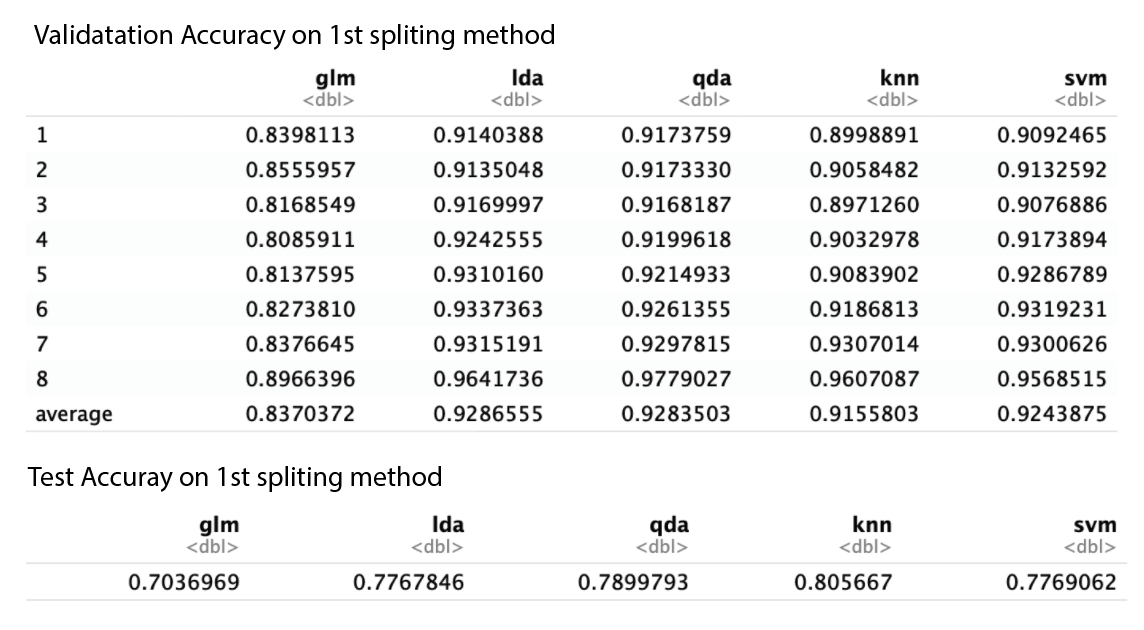
\includegraphics[width = 15.5cm]{3(a)1acuracy}

For the second one, the cross-validation average accuracies demonstrate that QDA have the best performance on validation data. QDA has a high accuracy on test data, but LDA performs better. GLM has lowest average cross-validation accuracy on validation set and svm performs worst on test data. Considering both average validation set accuracies and test set accuracies, we believe that QDA is also the best model for the second splitting method.

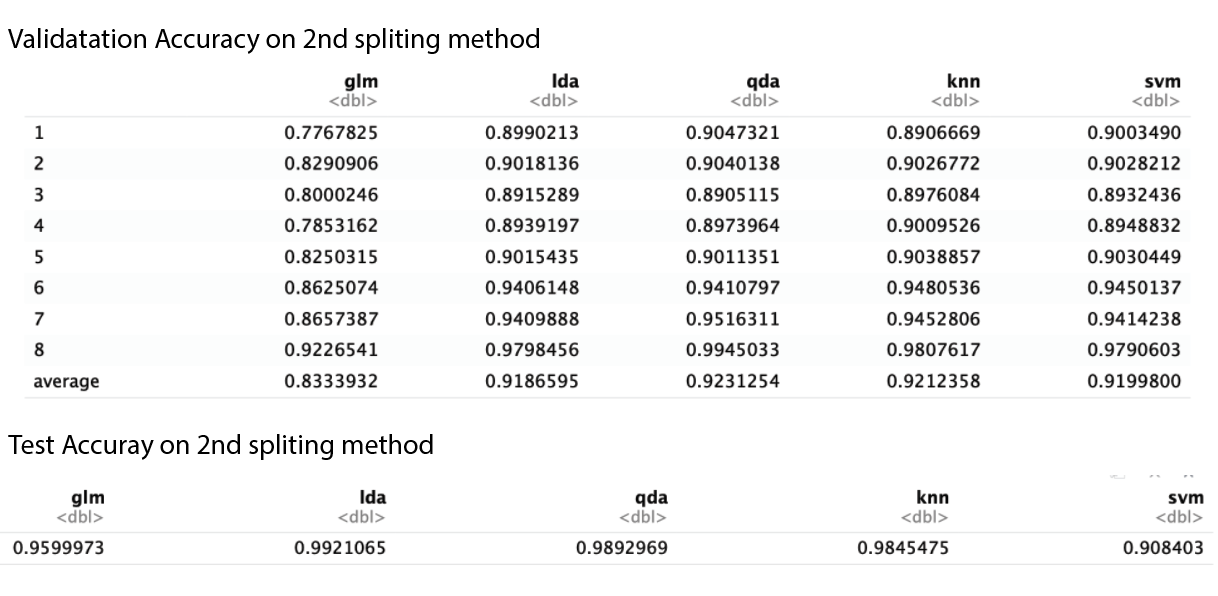
\includegraphics[width = 15.5cm]{3(a)2acuracy}

\vspace{0.3cm}
\mbox{}\\
\textbf{b. ROC curves}

We then plot ROC curves for each classification method. We don't plot a ROC curve for KNN, because the model does not calculate the probabily of being each class. It directly gives the classification result instead, and we don't really think it is worthy changing the hyperparameter K here. 

In each model, we choose the cutoff value that has the smallest distance to (0, 1). We do so because we want to maximize true positive rate and minimize false positive rate at the same time. We did not put more weight on true positive rate because, unlike the medical cases, the incorrect classifications of both clouded or cloud-free pixels have same consequence on our result.

To choose a best method according to the ROC curves, we calculate the distance between the point we marked and (0, 1). The smaller distance indicates a better model.

\mbox{}\\
The ROC curves are drawn below with cutoff value we choose marked for first splitting method:

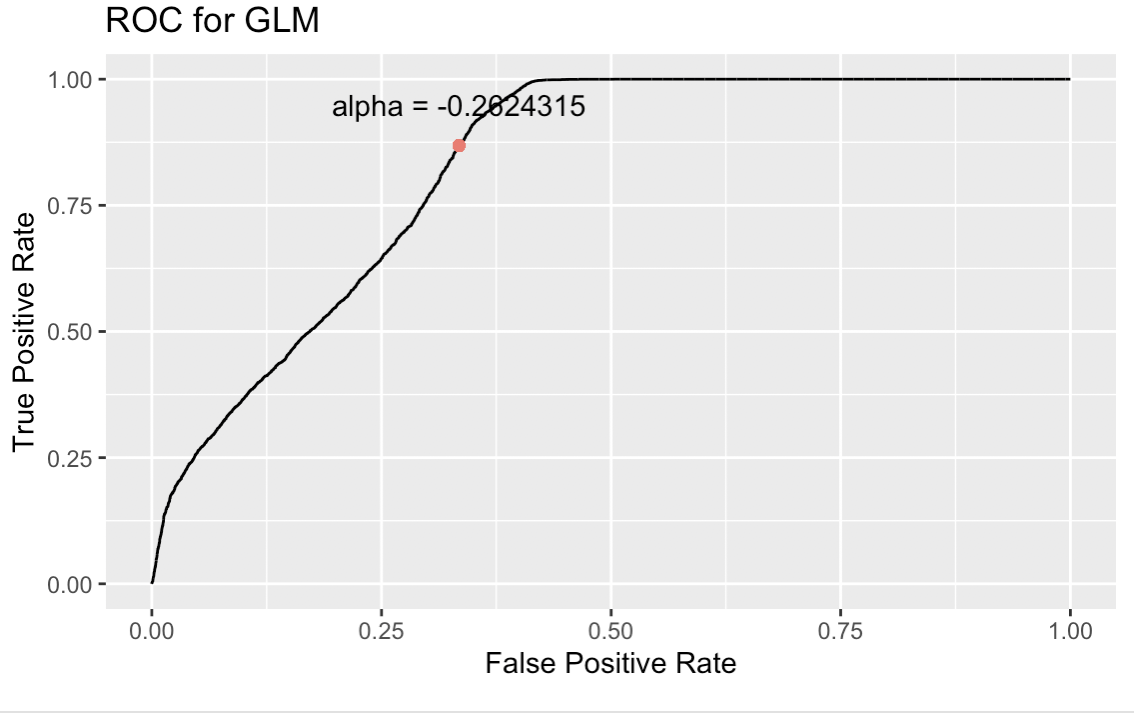
\includegraphics[width = 7.5cm]{3(b)1-1}
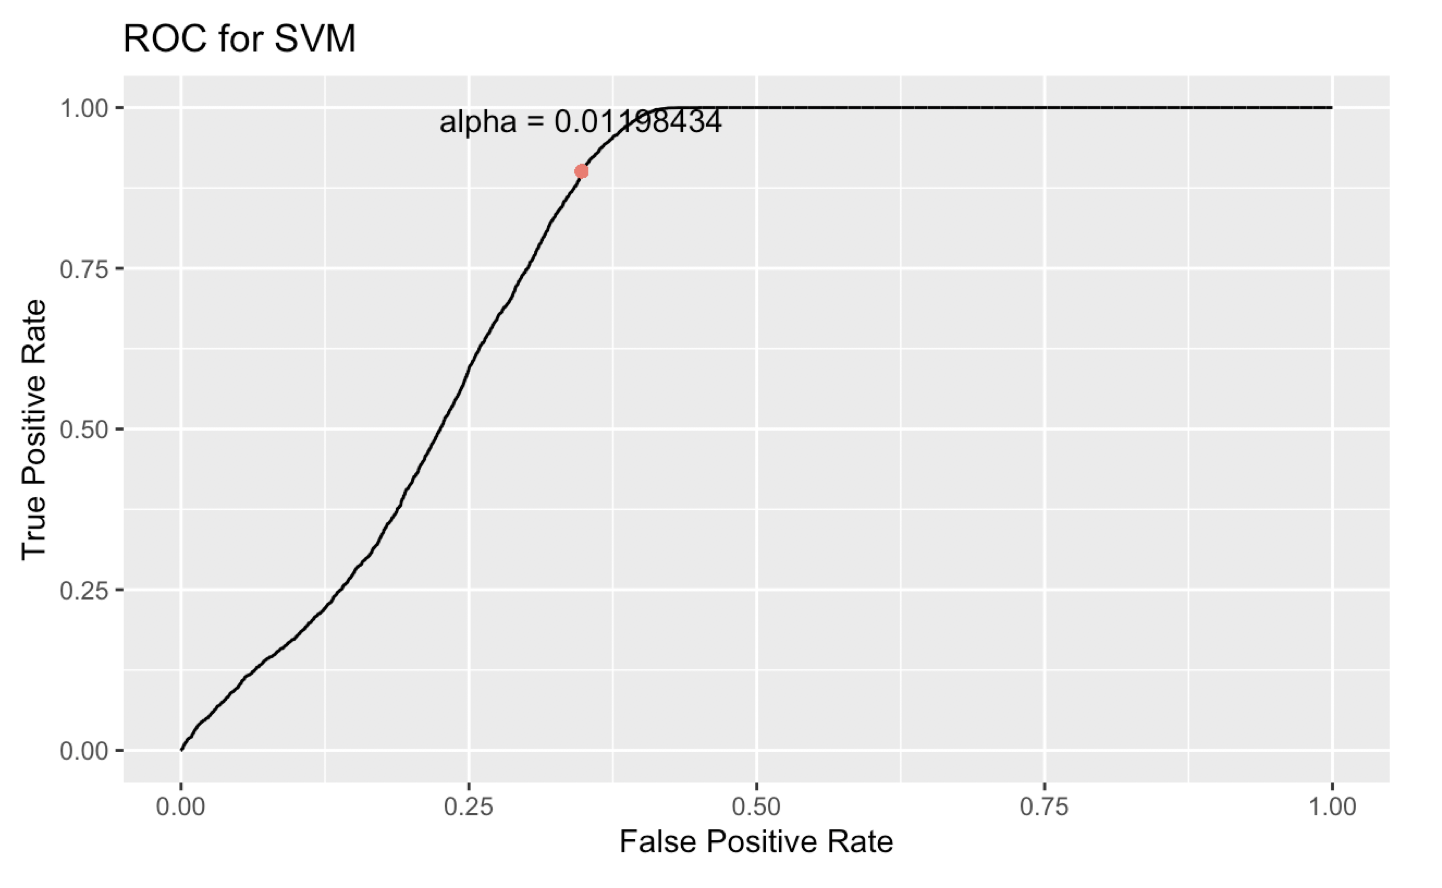
\includegraphics[width = 7.5cm]{3(b)1-2}

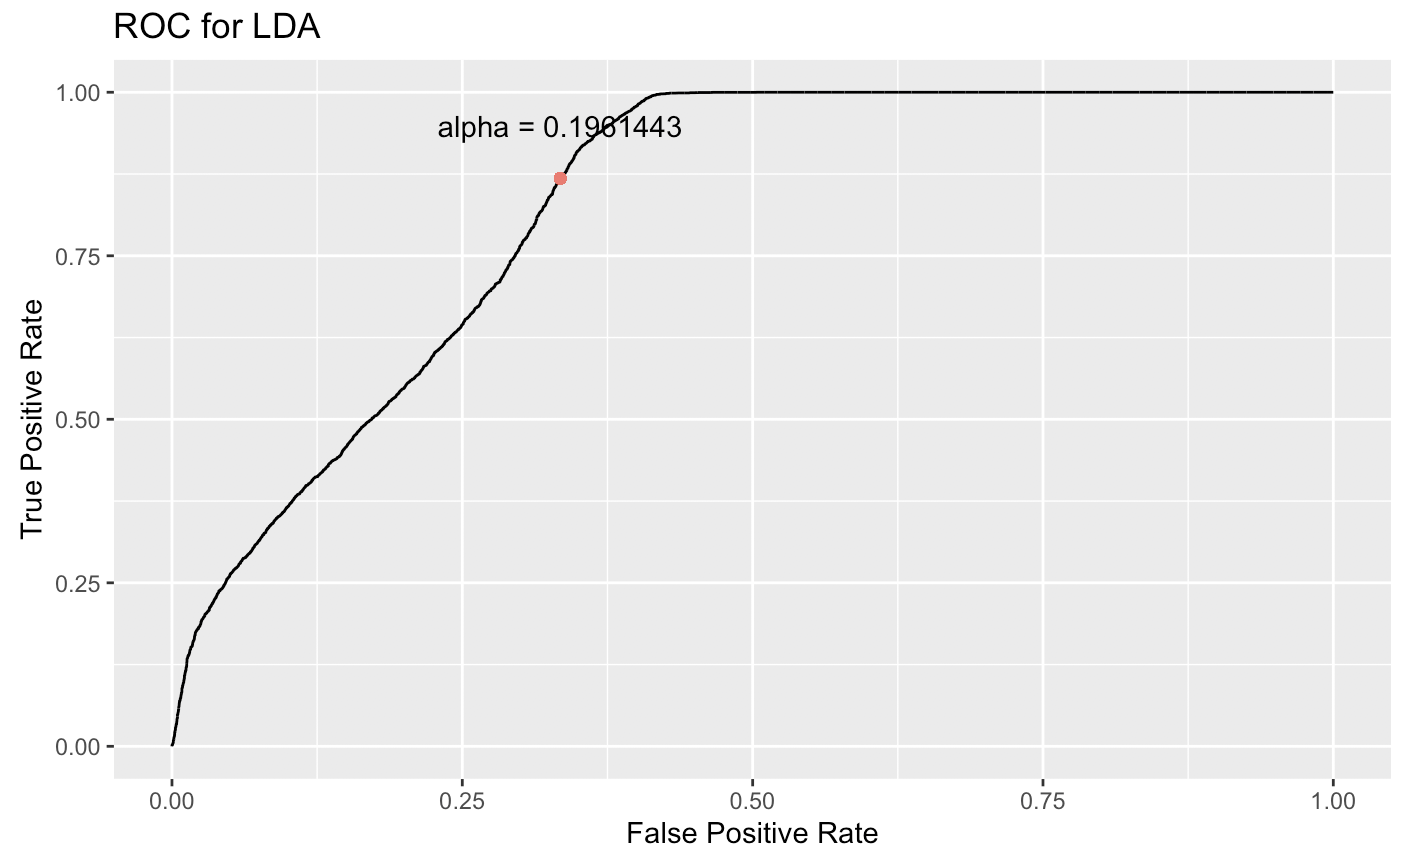
\includegraphics[width = 7.5cm]{3(b)1-3}
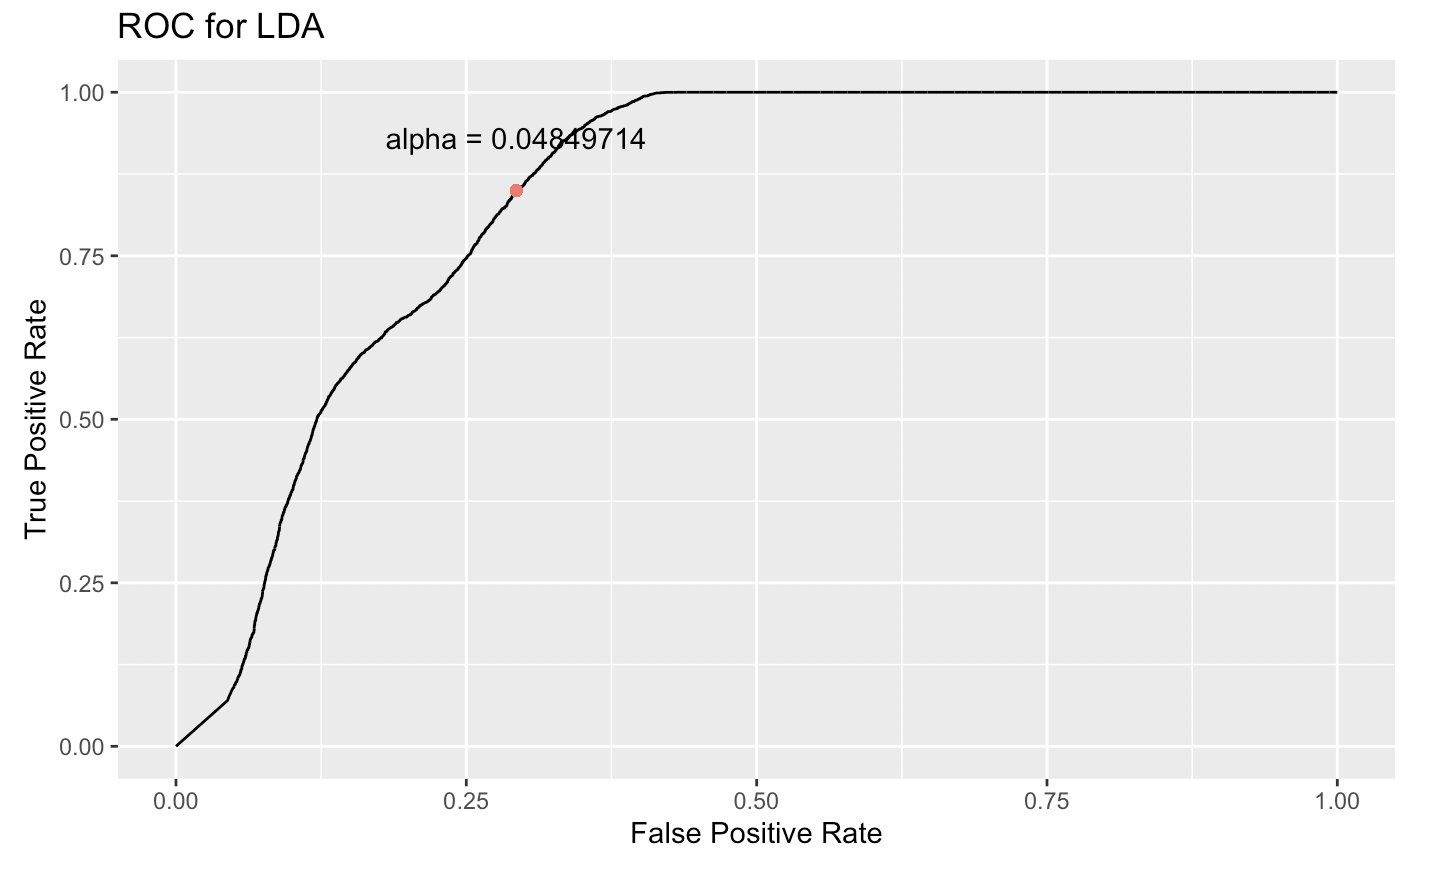
\includegraphics[width = 7.5cm]{3(b)1-4}

In the first spliting method, GLM and LDA both have the shortest distance 0.1291 to the point (0,1) and the same value 0.8239 for the area under the ROC curve value.SVM returns a slightly larger distance 0.1296 but covers the least area under the ROC curve with value 0.7854. QDA gives the largest distance 0.1637 to the point (0,1) and the largest AUC value 0.8391. Noticed that the ROC curves for four models are not smooth and some curves are slightly convex, which are different from usual ROC curve. This is because the cloud data set cannot be separated with a linear combination of featues. All our models assume that the data are linear separable, which might result in the abnormal shape of the RUC cruve.  

Similarly, we analyze the the ROC curves for second spliting method:

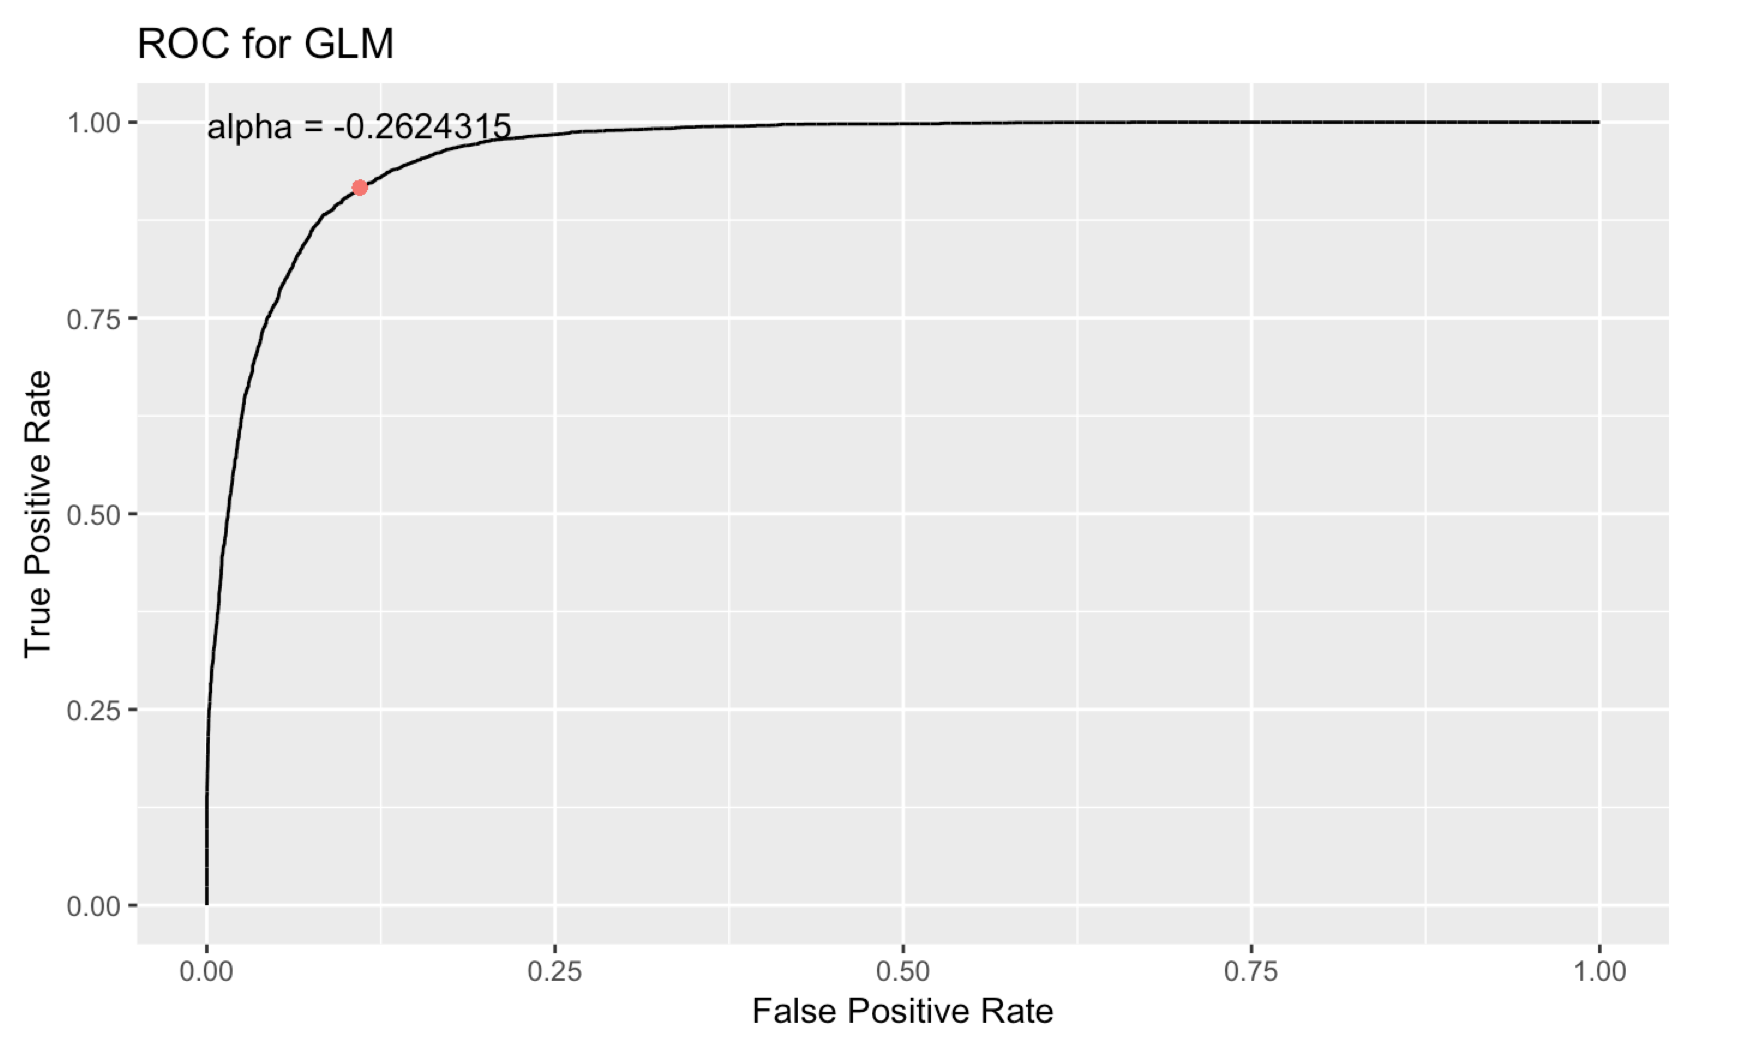
\includegraphics[width = 7.5cm]{3(b)2-1}
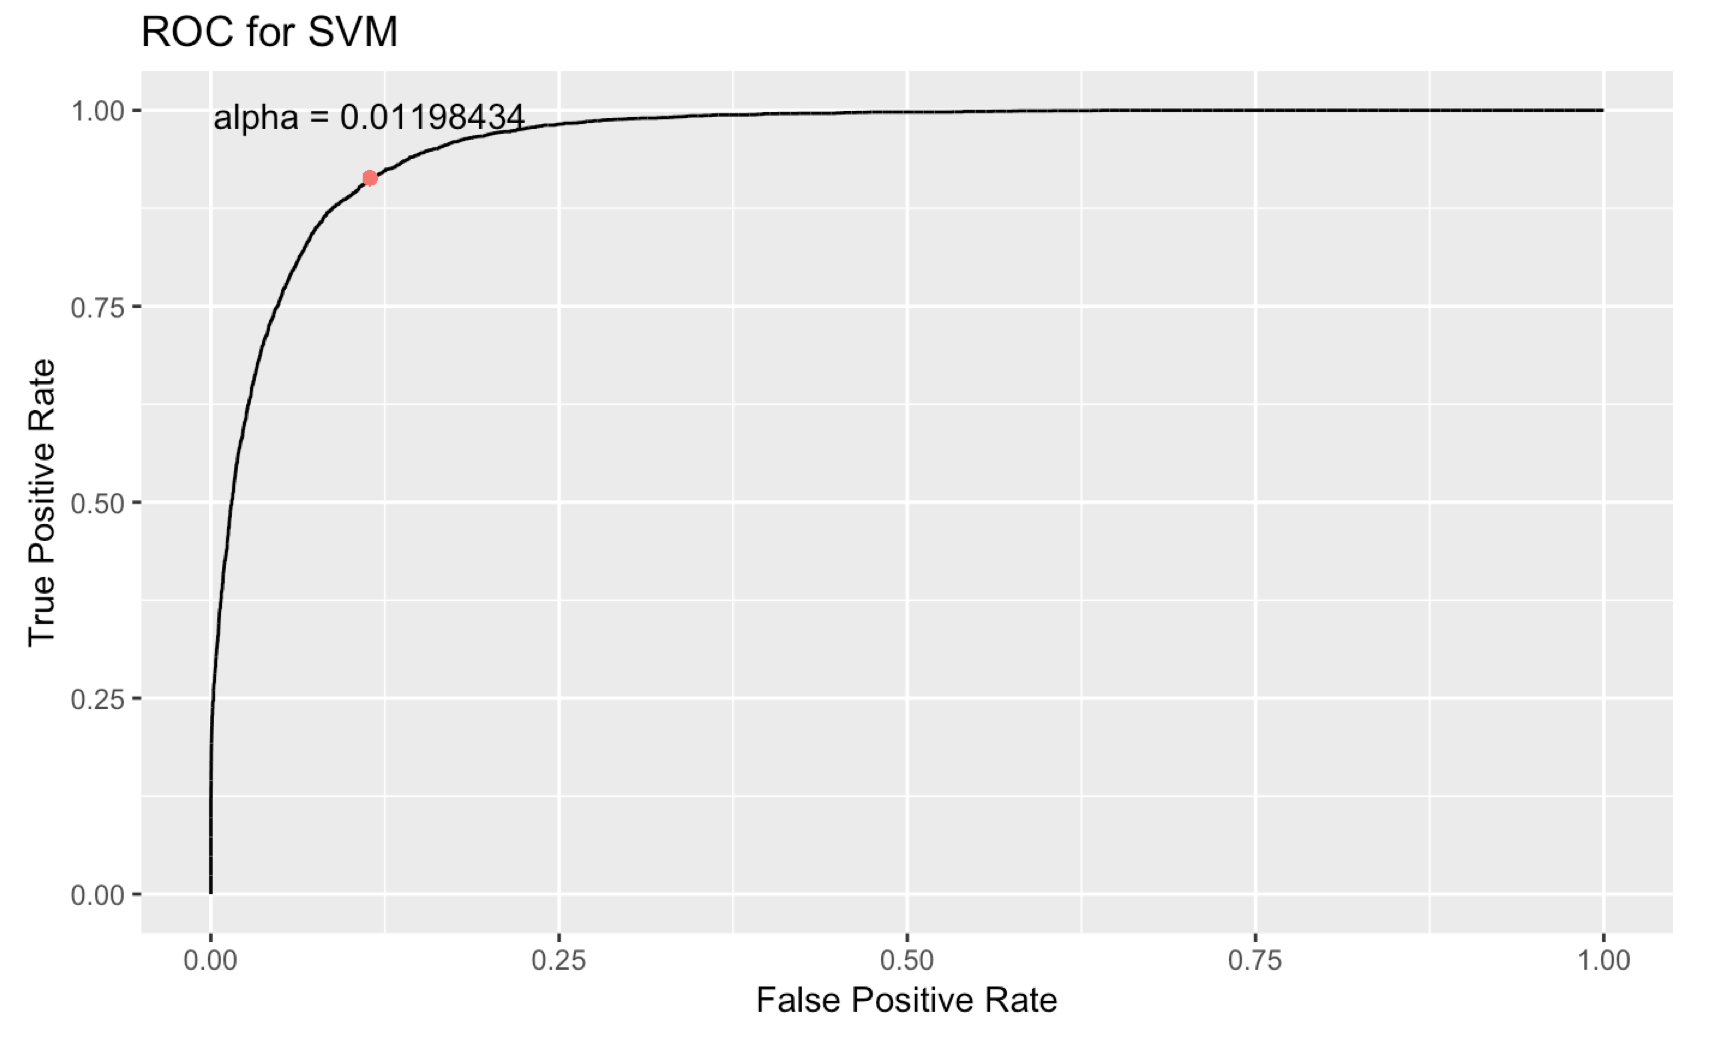
\includegraphics[width = 7.5cm]{3(b)2-2}

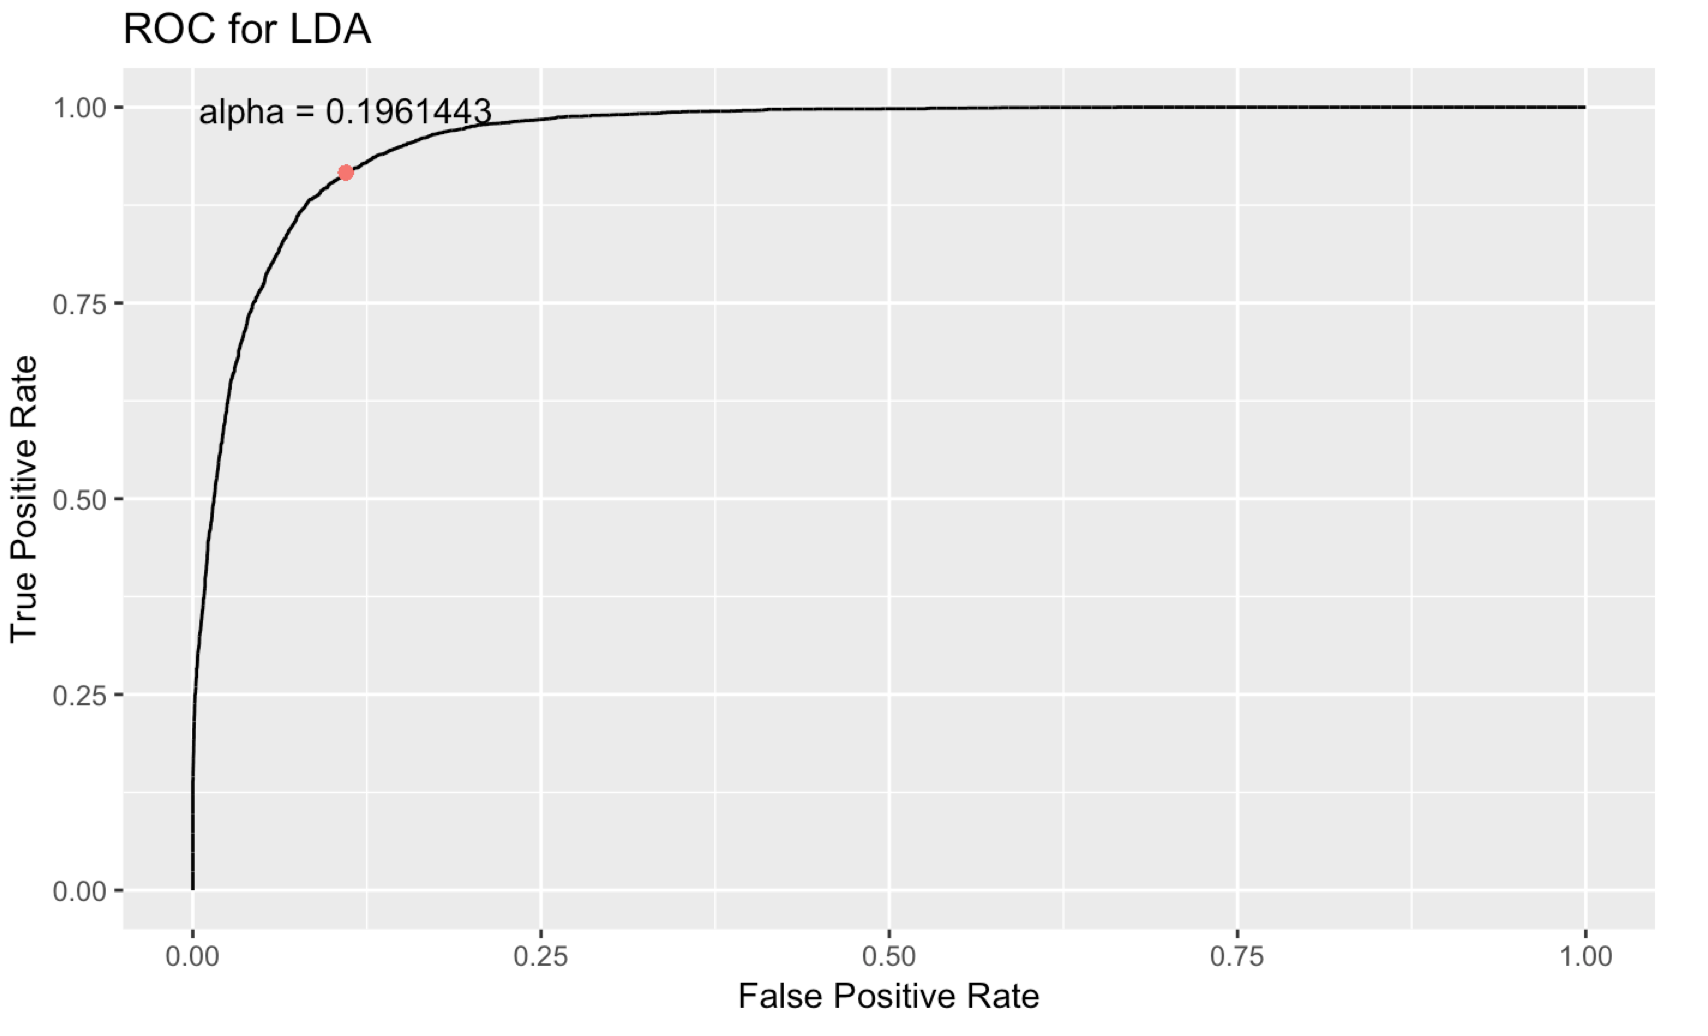
\includegraphics[width = 7.5cm]{3(b)2-3}
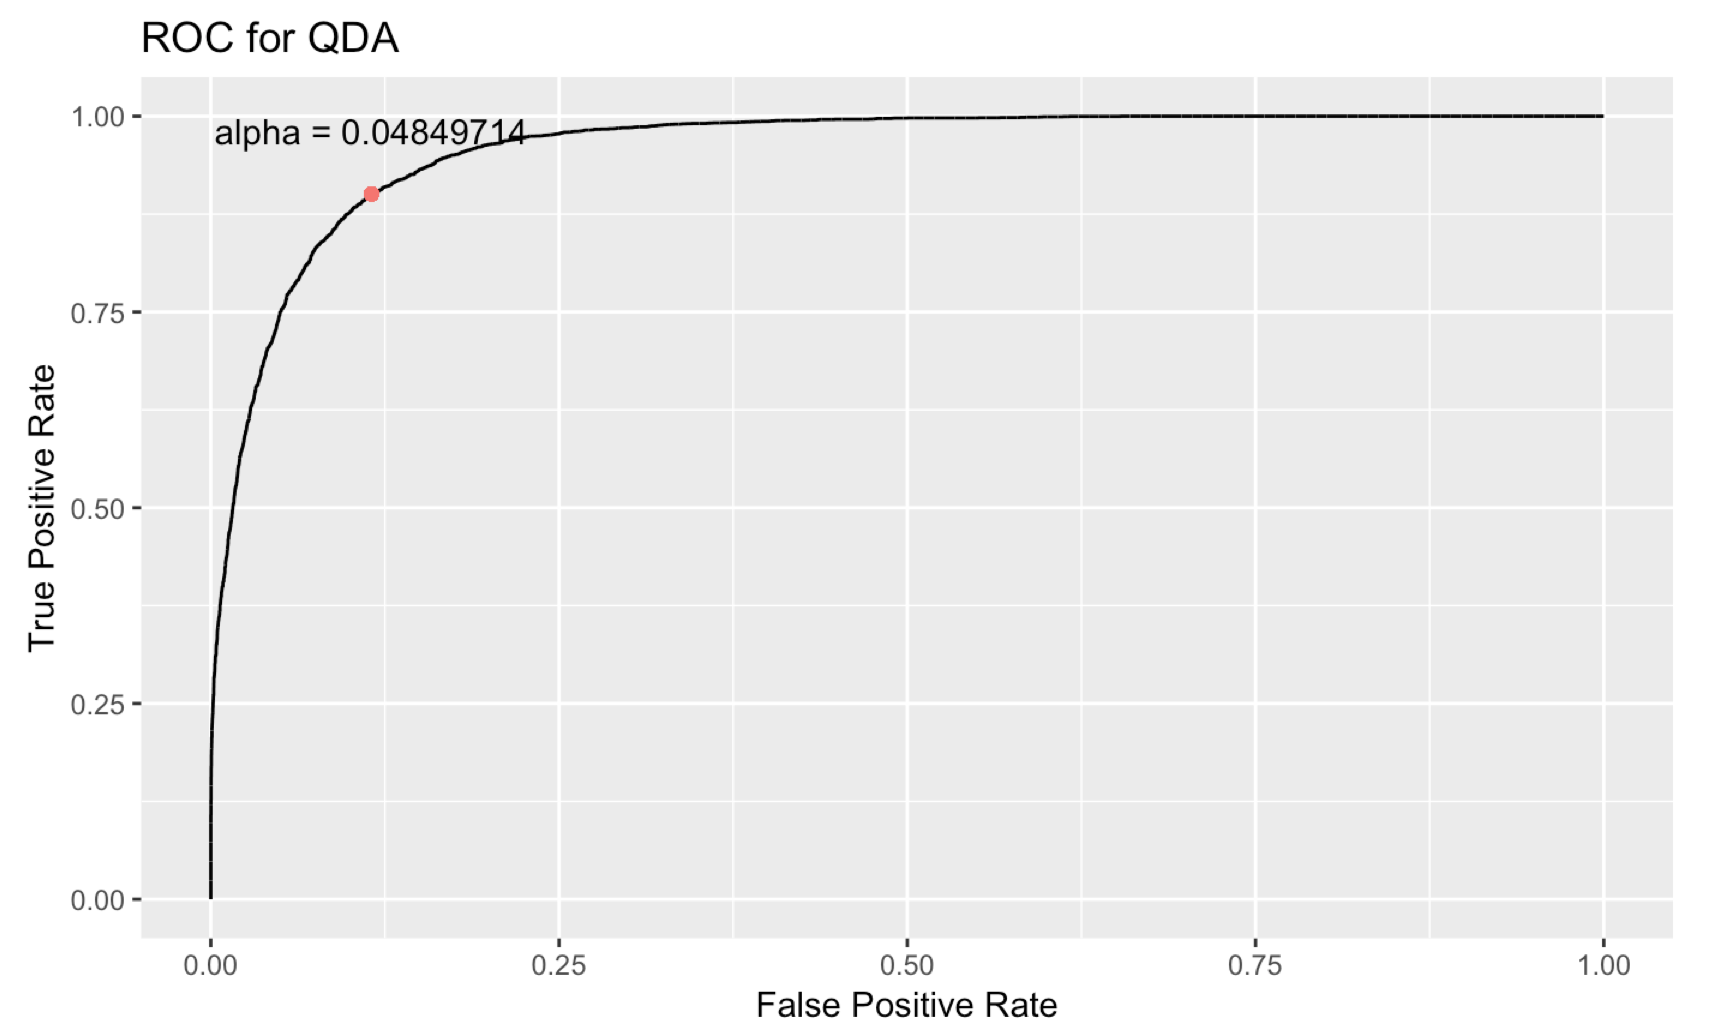
\includegraphics[width = 7.5cm]{3(b)2-4}

In the second spliting method, GLM has a distance of 0.019, SVM has a distance of 0.021, LDA has a distance of 0.019, QDA has a distance of 0.023. The distances of different methods does not change very much. Then, we also calculate the AUC for each classification method. The larger AUC indicate a better model. The area under GLM's ROC curve is 0.9635, the area under SVM's ROC curve is 0.9613, the area under LDA's ROC curve is 0.9635 and the area under QDA's ROC curve is 0.9581. Considering both of these two factors, for the second splitting method, we think GLM and LDA are better than the rest of two.



\section{Diagnostics}

\vspace{0.2cm}
\textbf{a. In-depth Analysis}

According to the analysis above, we think second splitting method is better and QDA is the best classification method in our case. Therefore, we do some in-depth analysis on QDA for the second splitting method.

The means and covariances of each class are shown as follows:

\mbox{}\\
Mean and Covariance matrix for design matrix classified as cloud

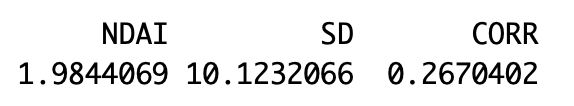
\includegraphics[width = 7.5cm]{4(a)1}
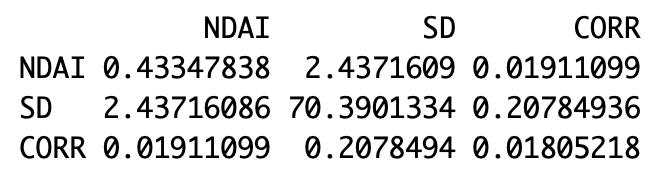
\includegraphics[width = 7.5cm]{4(a)2}

\mbox{}\\
Mean and Covariance matrix for design matrix classified as cloud-free

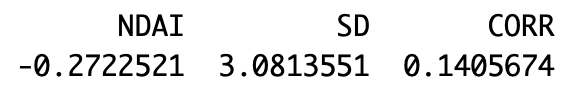
\includegraphics[width = 7.5cm]{4(a)3}
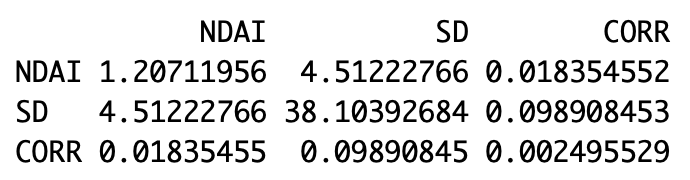
\includegraphics[width = 7.5cm]{4(a)4}

The high variances (covariances between features themselves) means that the corresponding features have a lot of expressiveness. In other words, features with low variances are close to a constant. In our case, we prefer features with larger variances. For the rest covariances (covariances between different features), features with high covariances have a lot of redundancy for each other. Since we hope the features can capture as much as possible, we prefer features with low covariances.

In our covariance matrices, SD has very high variance and relatively low covariance. SD is the best feature of these three. CORR has lowest variance and relatively high covariance. We may want to improve our model by changing this feature to another.

\vspace{0.3cm}
\mbox{}\\
\textbf{b. Misclassification Analysis}

For our best classification model which is QDA, we analyze the misclassification by showing ranges of feature values. We also apply our trained model to three different image data sets and plot the misclassified data point on the original map to check if they are in particular regrions.

In the test data, we pick all misclassified data points and plot boxplots for each feature based on two different classification errors (False Positive and False Negative).

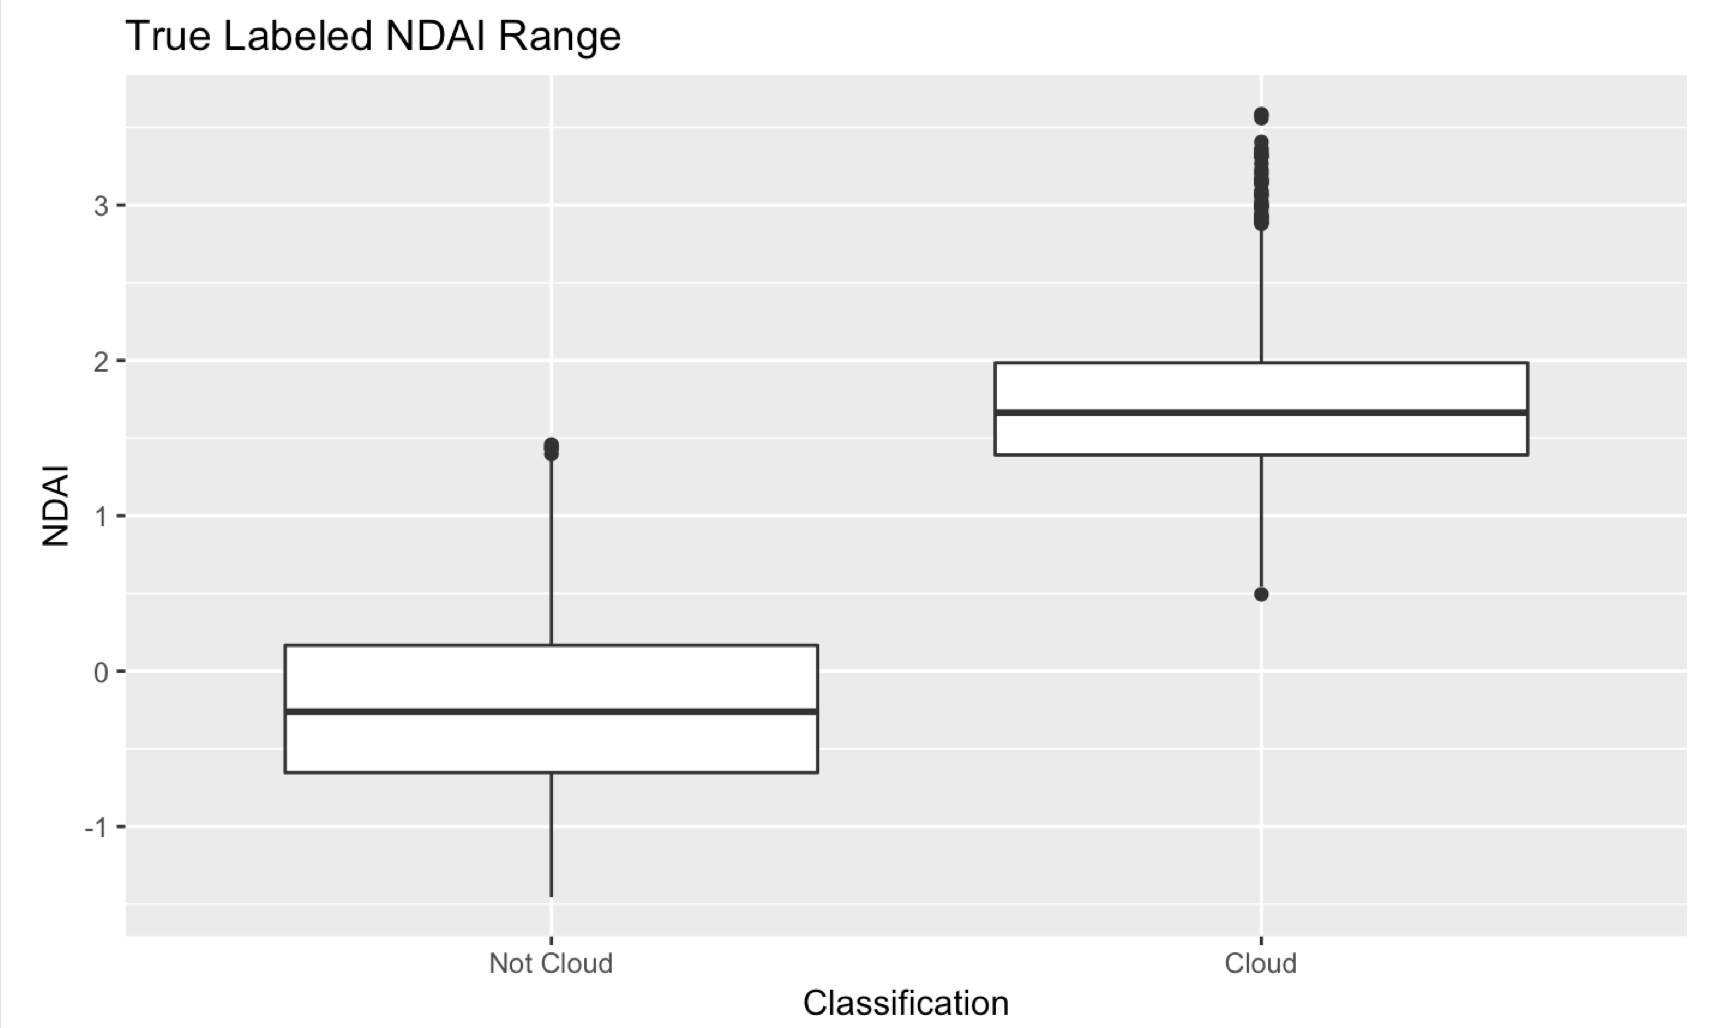
\includegraphics[width = 7.5cm]{4(b)1}
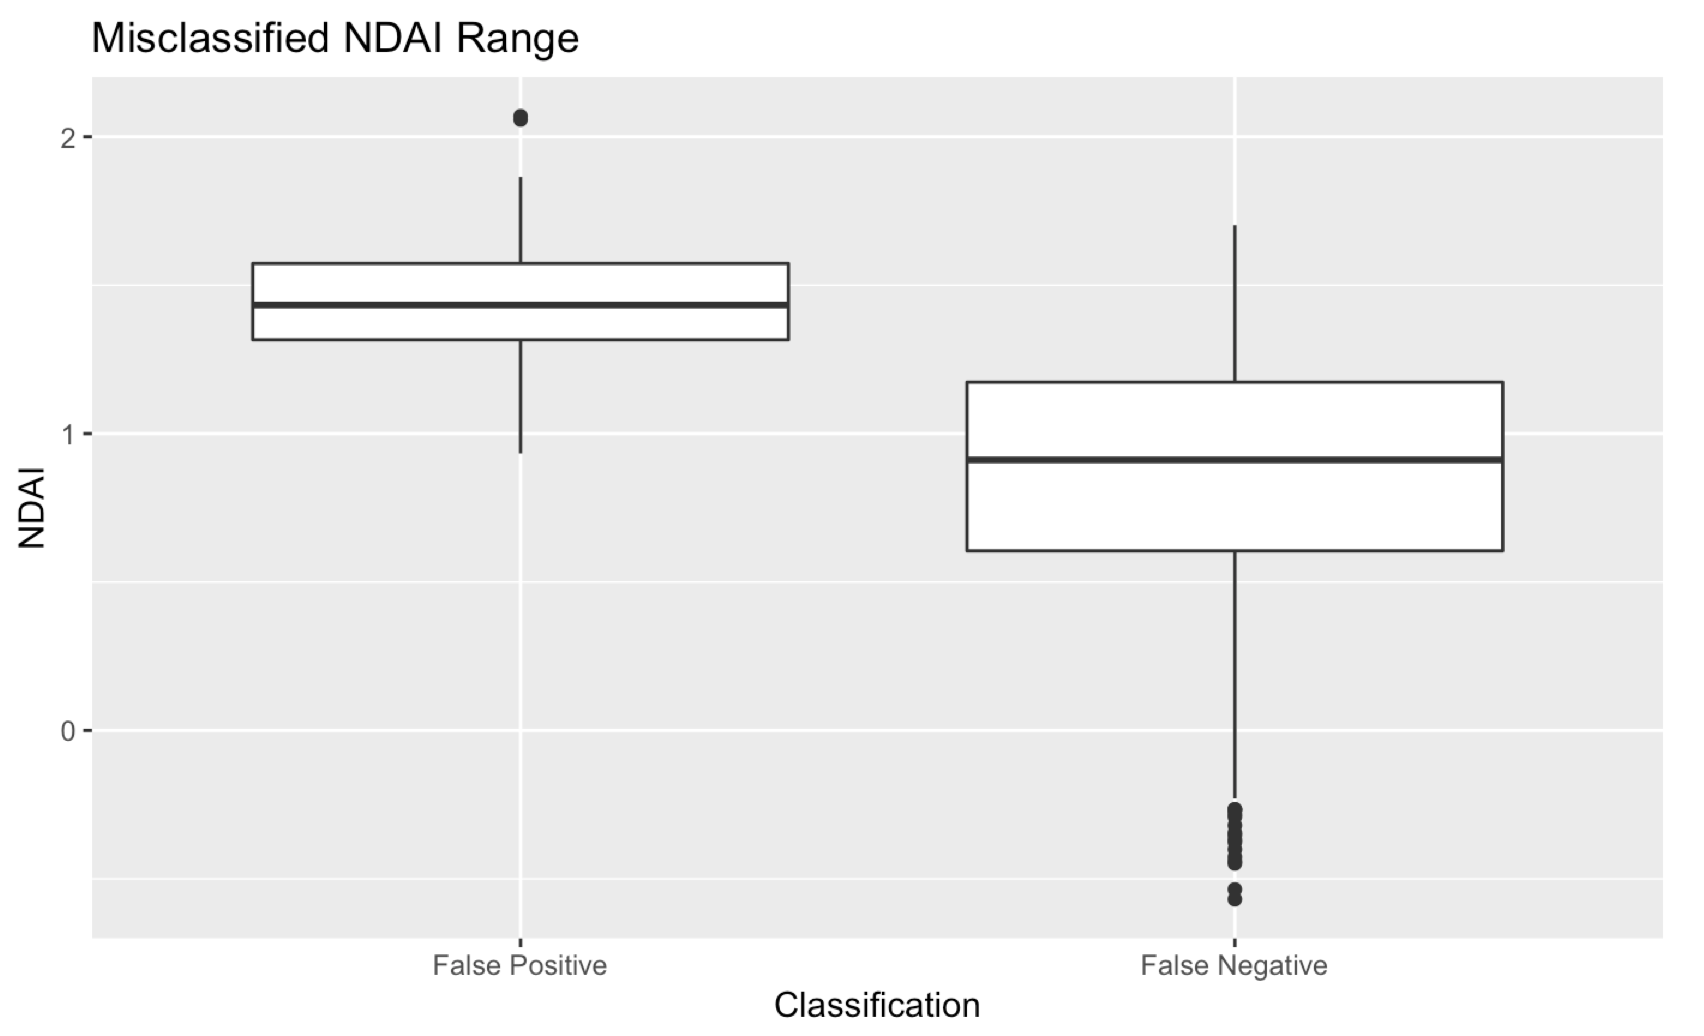
\includegraphics[width = 7.5cm]{4(b)2}

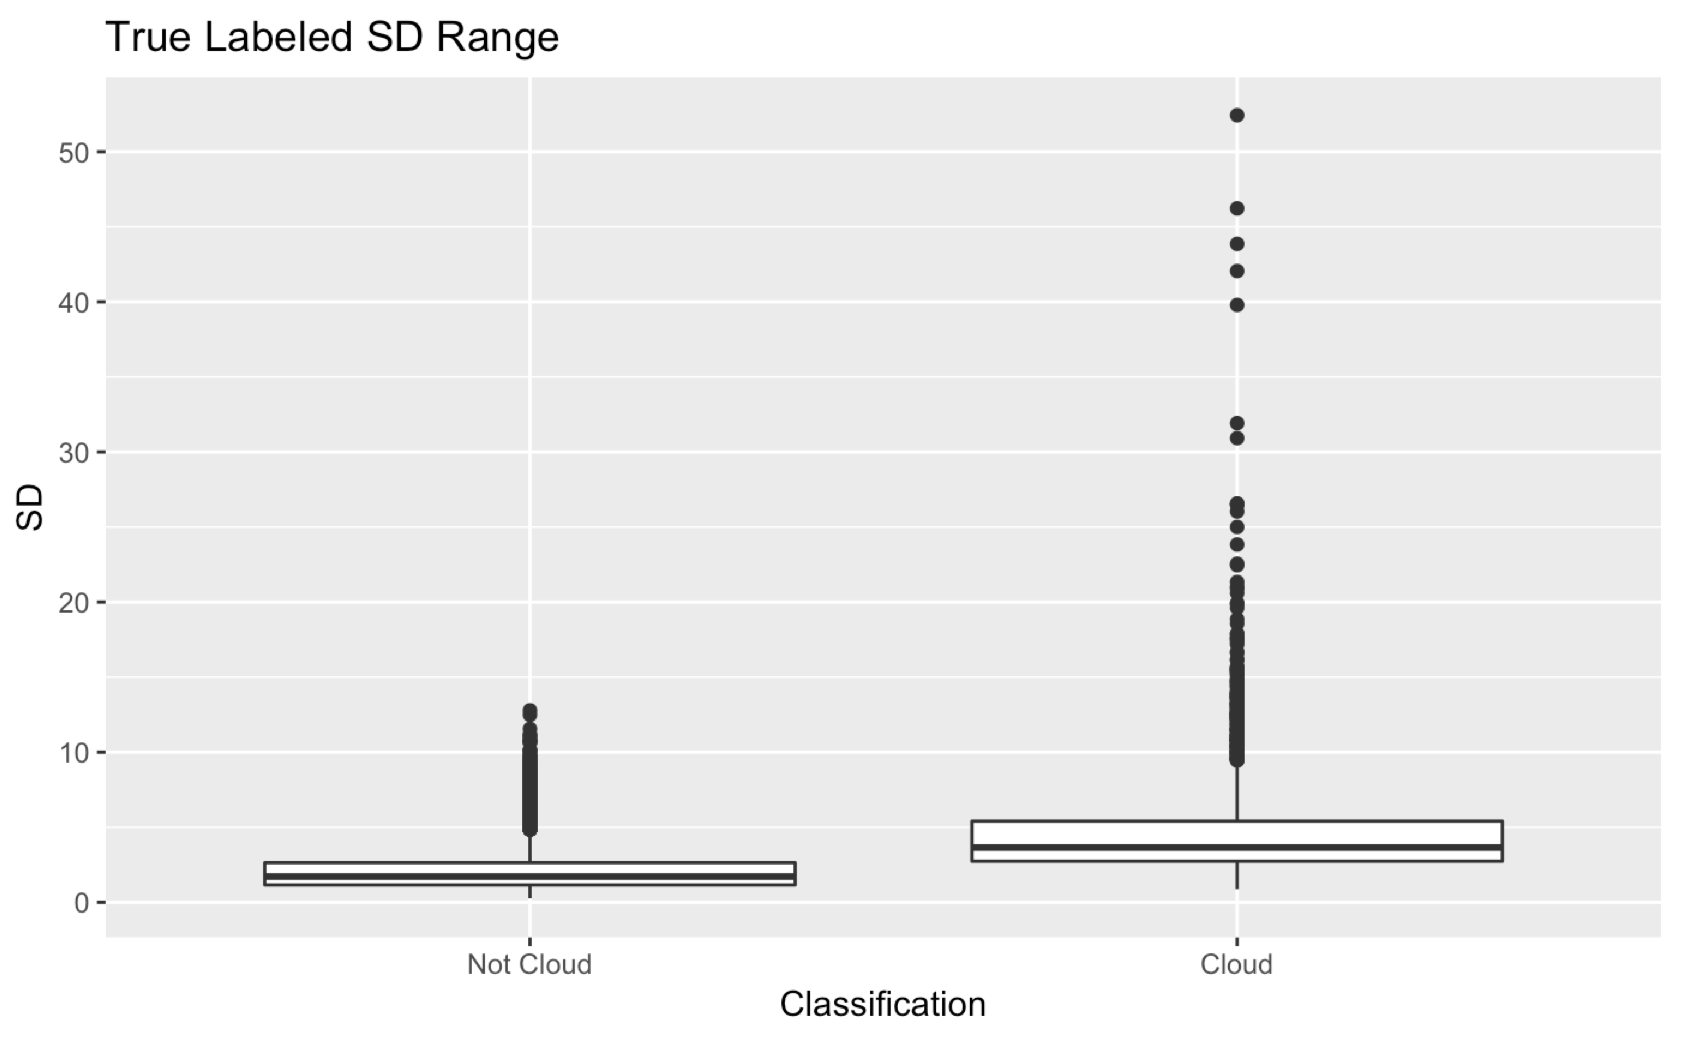
\includegraphics[width = 7.5cm]{4(b)3}
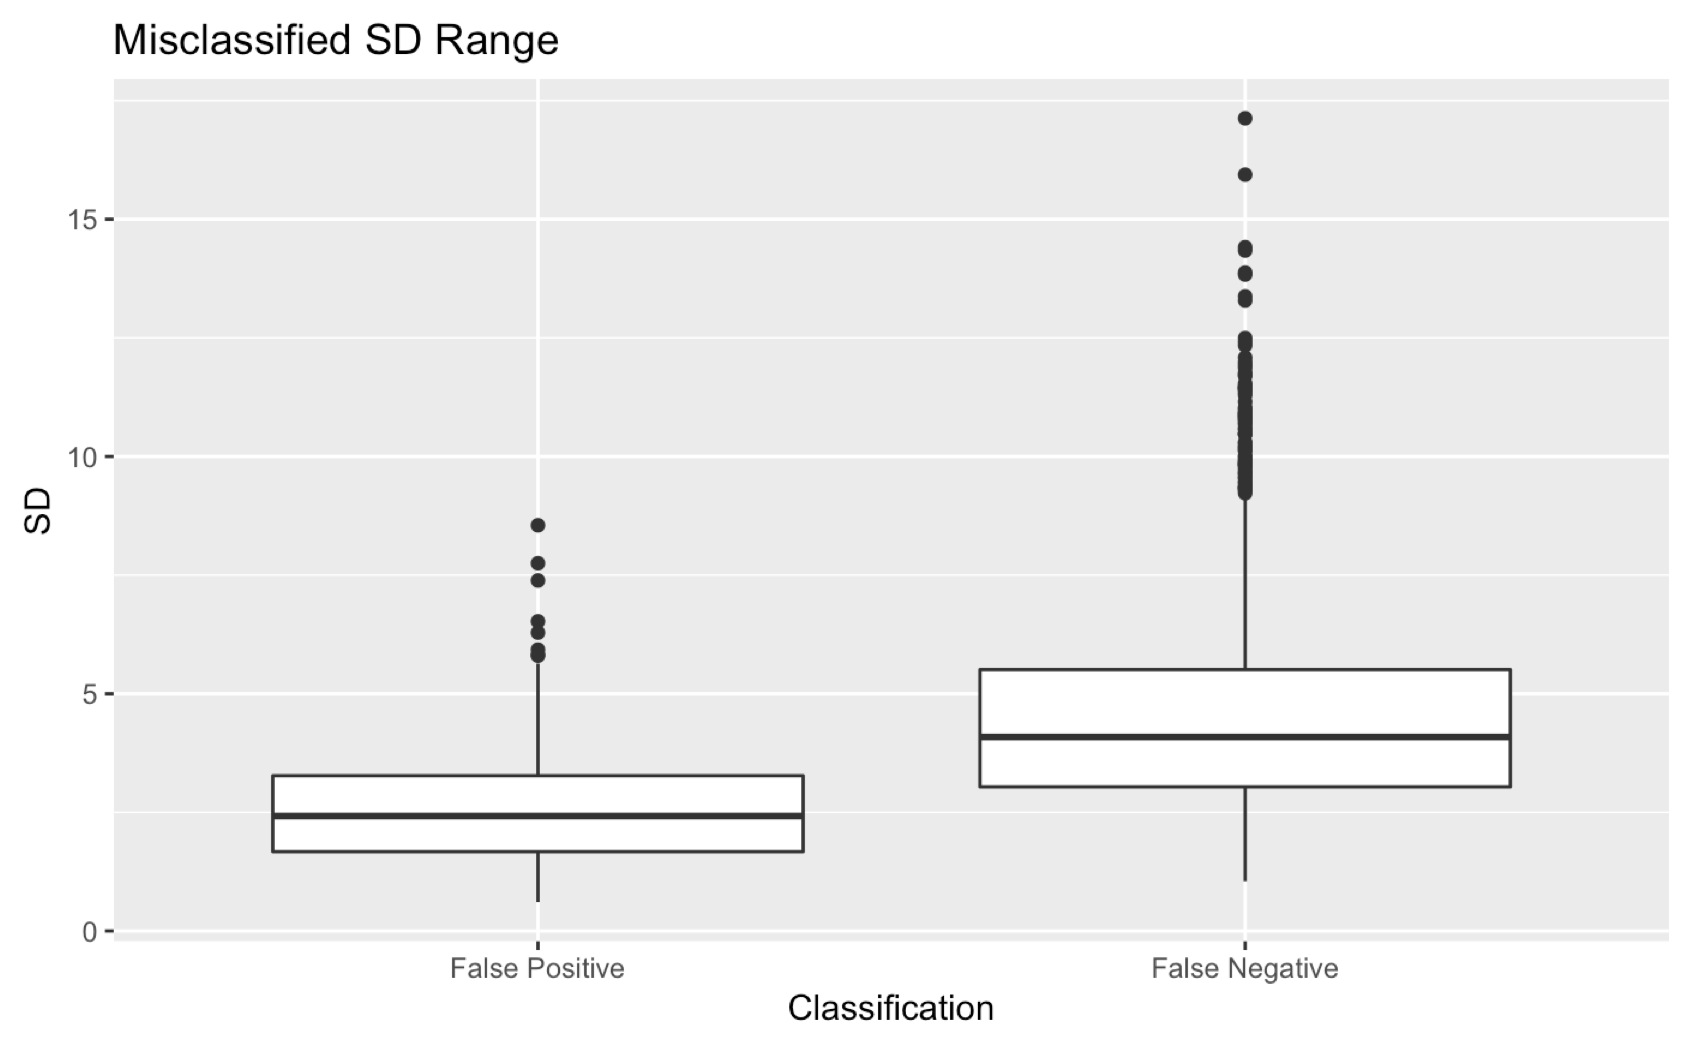
\includegraphics[width = 7.5cm]{4(b)4}

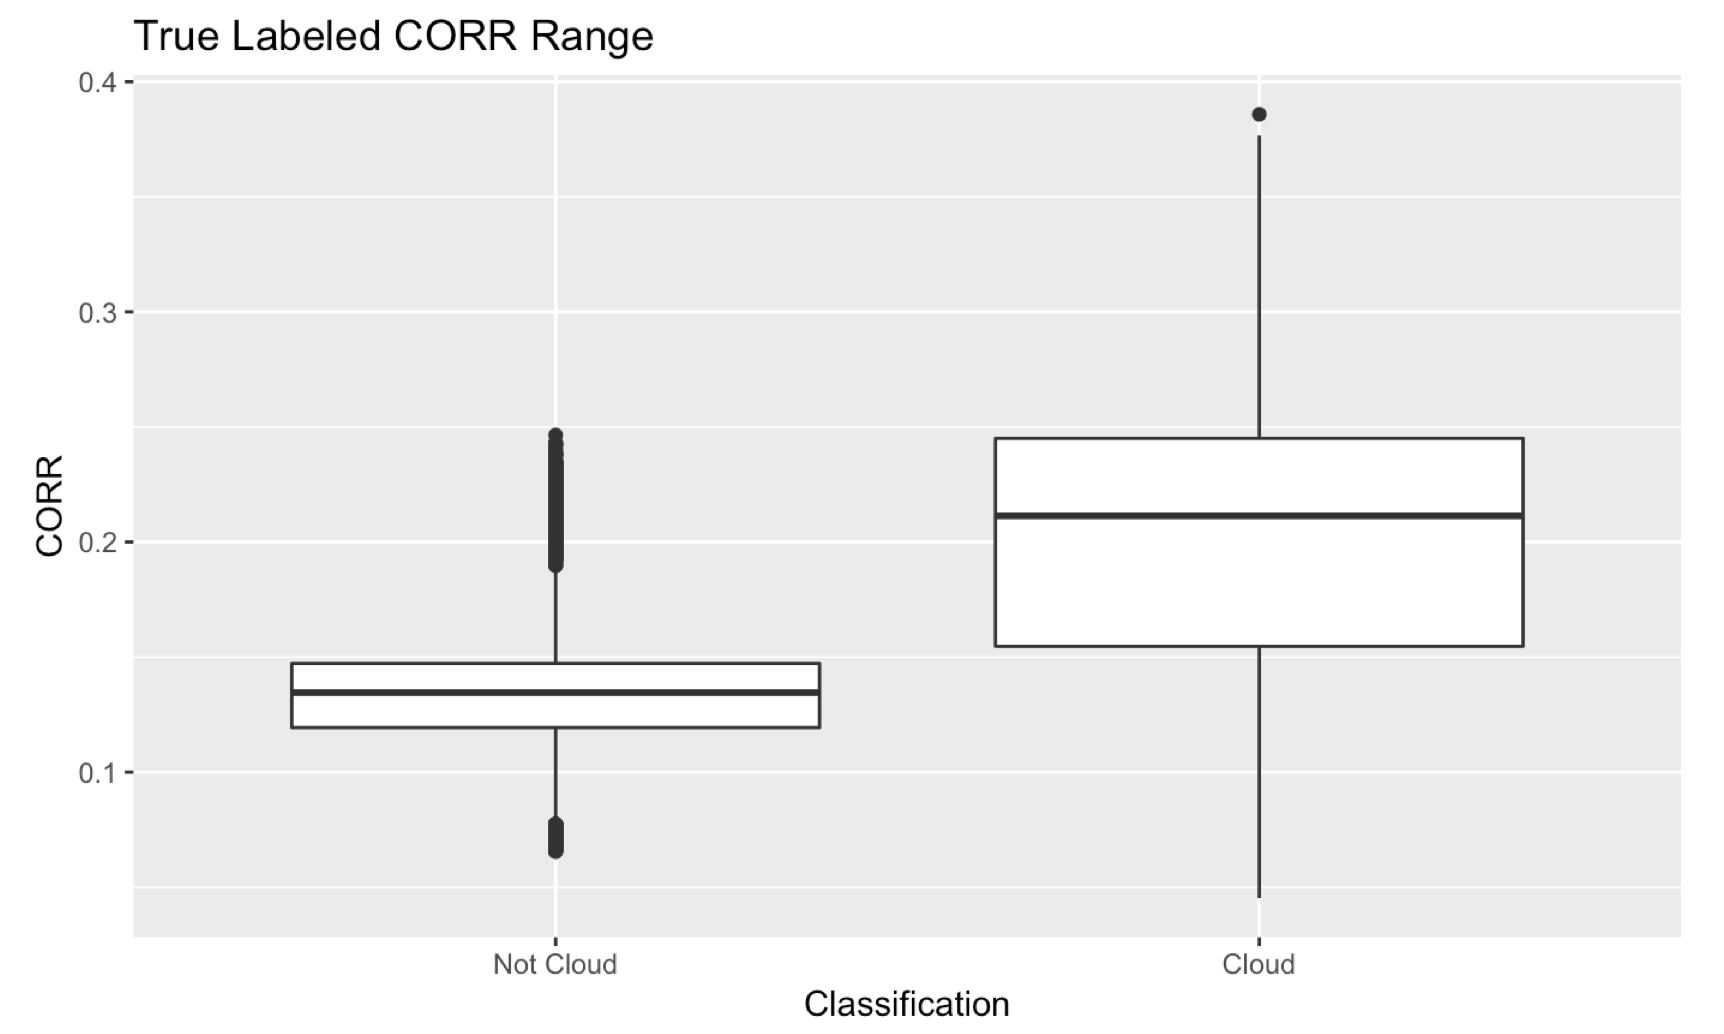
\includegraphics[width = 7.5cm]{4(b)5}
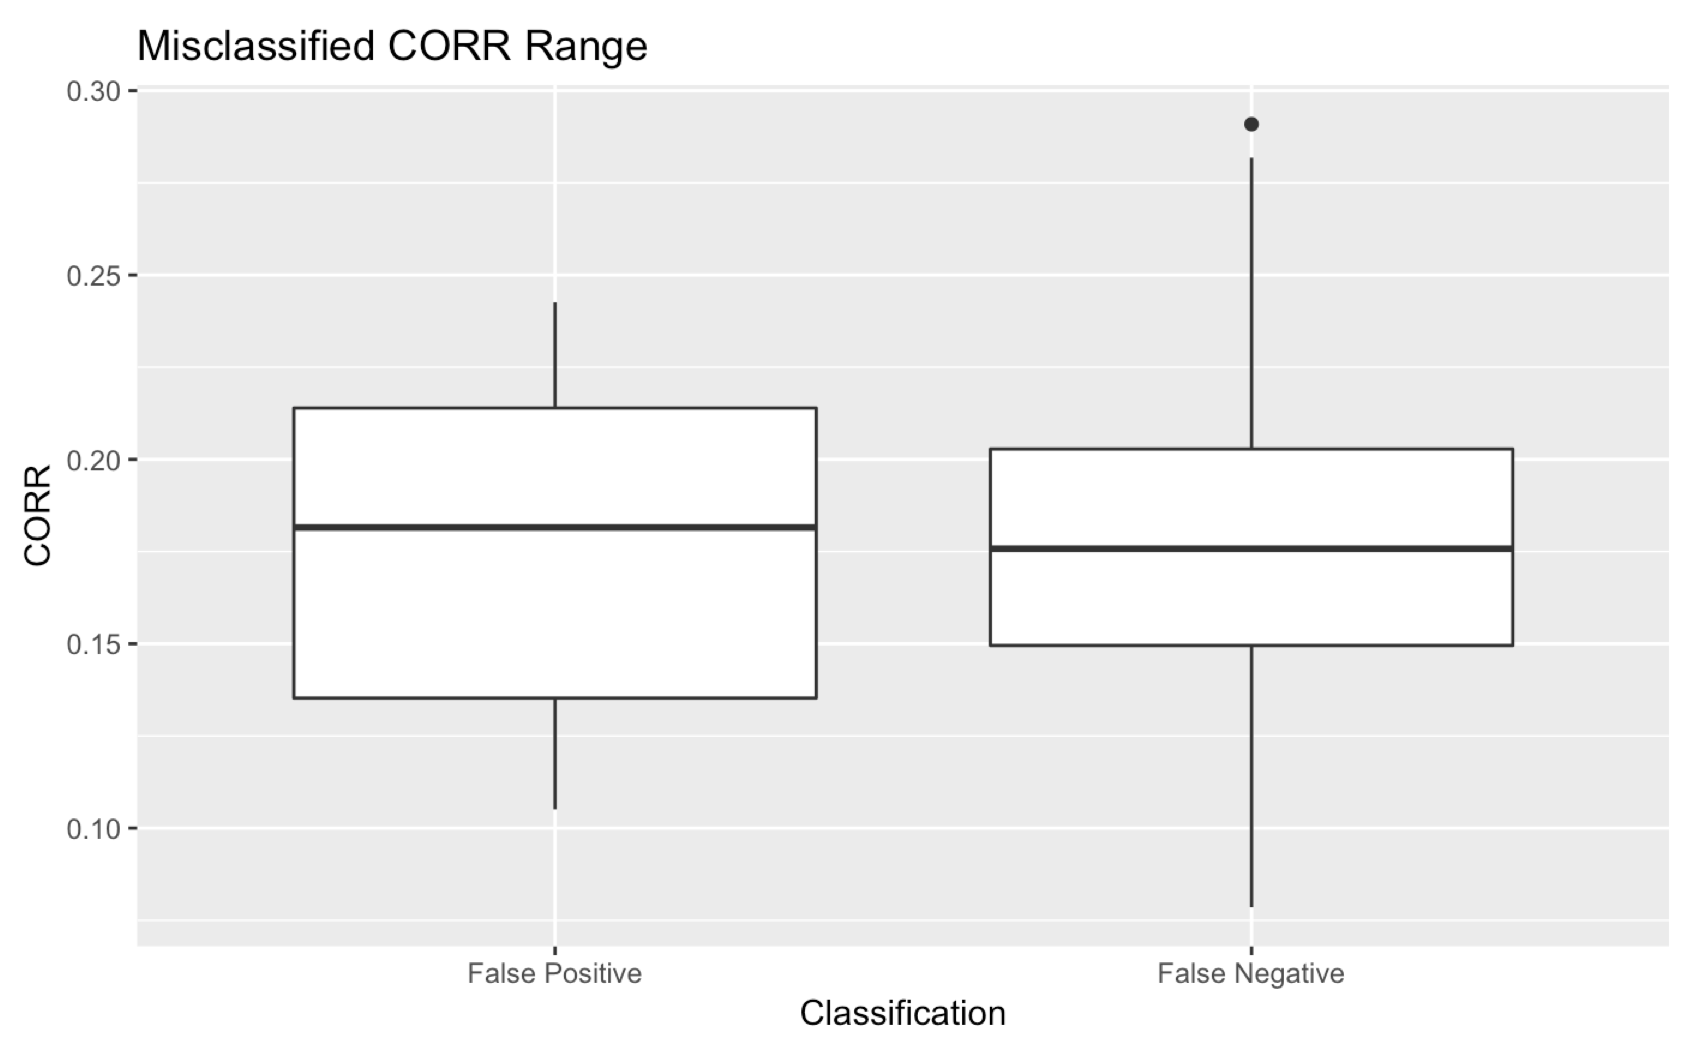
\includegraphics[width = 7.5cm]{4(b)6}

The plot on the left is the data correctly classified and the plot on the right are those misclassified. Comparing groups of distributions (Not Cloud vs. False Positive \& Cloud vs. False Negative) for NDAI, we see they have a different range and are differently distributed, which means the mispredicted data have a partiular pattern on this feature. Thus, we can conclude that our model can easily predict data with cloud as not clouded when their NDAI have high values and more tend to predict data without cloud as clouded when their NDAI have extremely low value. 

The data in plots for SD have quite similar distributions for both groups. However, we have very different range particularly for the False-negative boxplot, which means, when SD is very low, our model can very easily predict pixels with cloud as non-clouded.

And finally for CORR, we have similar distributions for Cloud and false-negative boxplots but have different distributions for not-cloud and false-positive boxplots. Our model tend to predict some pixels with high CORR as cloud-free. This can be explained by the phenonmenon that pixels have high correlation for cloud-free areas. 

Then, we use our trained QDA model to predict data points in three image data sets (data points with expert label of 0 are excluded). And plot the predicted labels for each image data set.

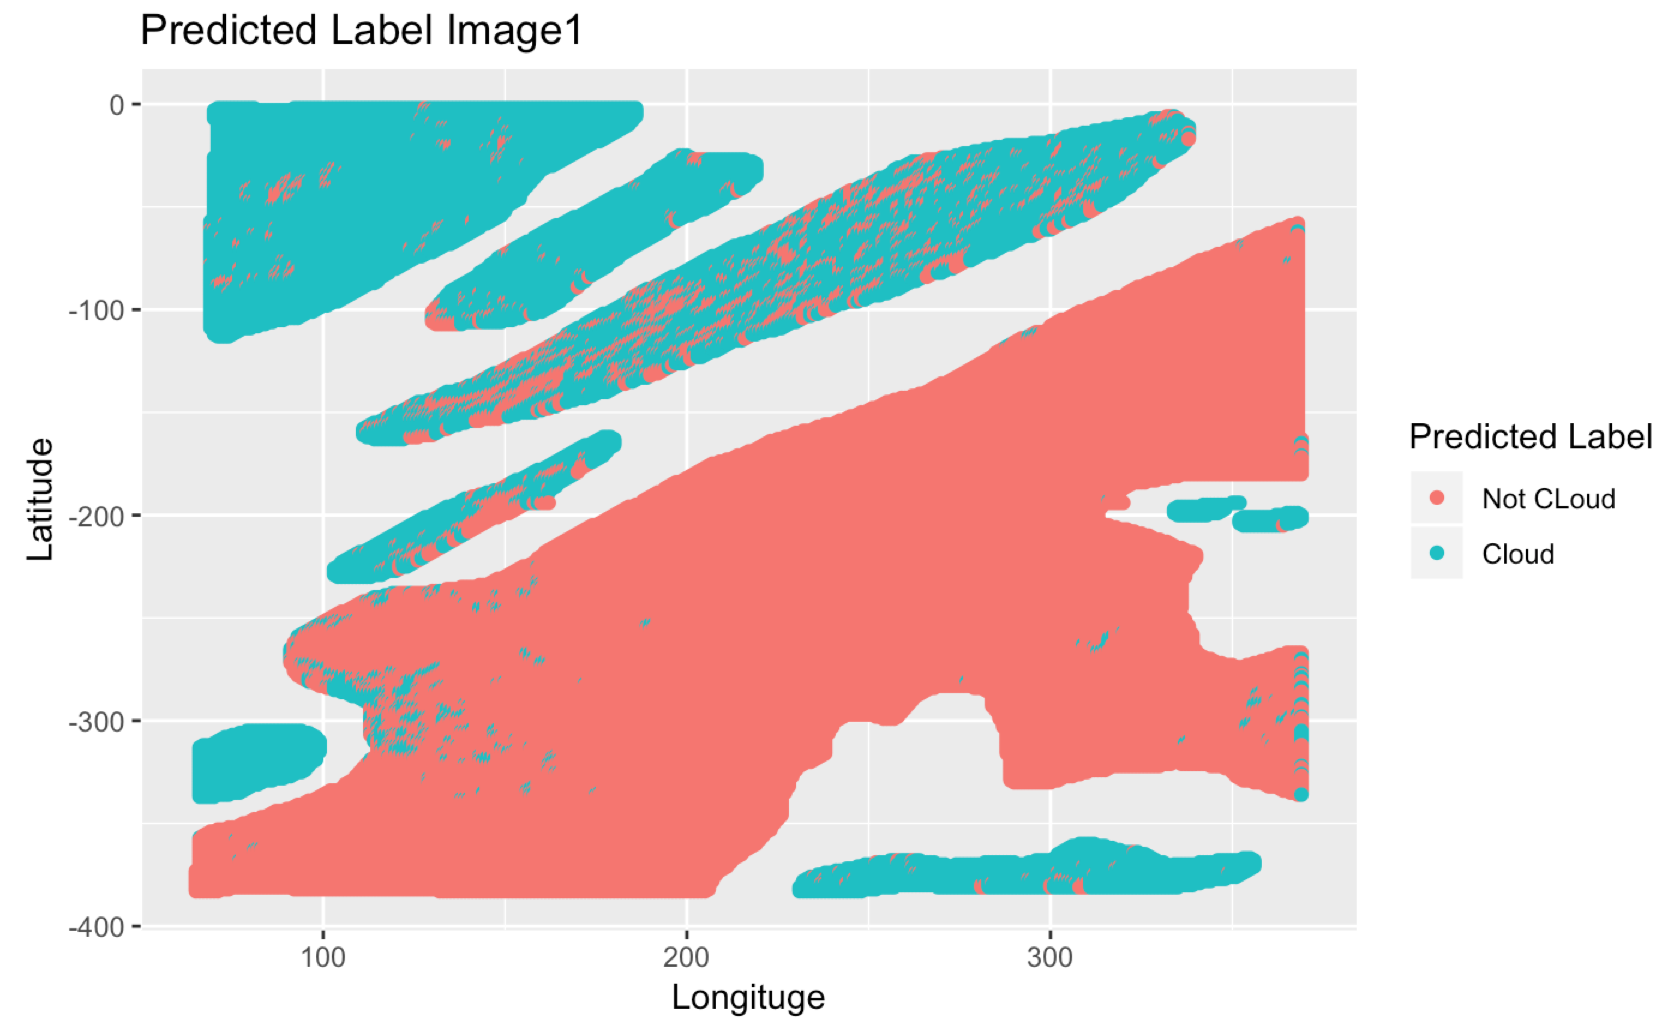
\includegraphics[width = 6cm]{4(b)7}
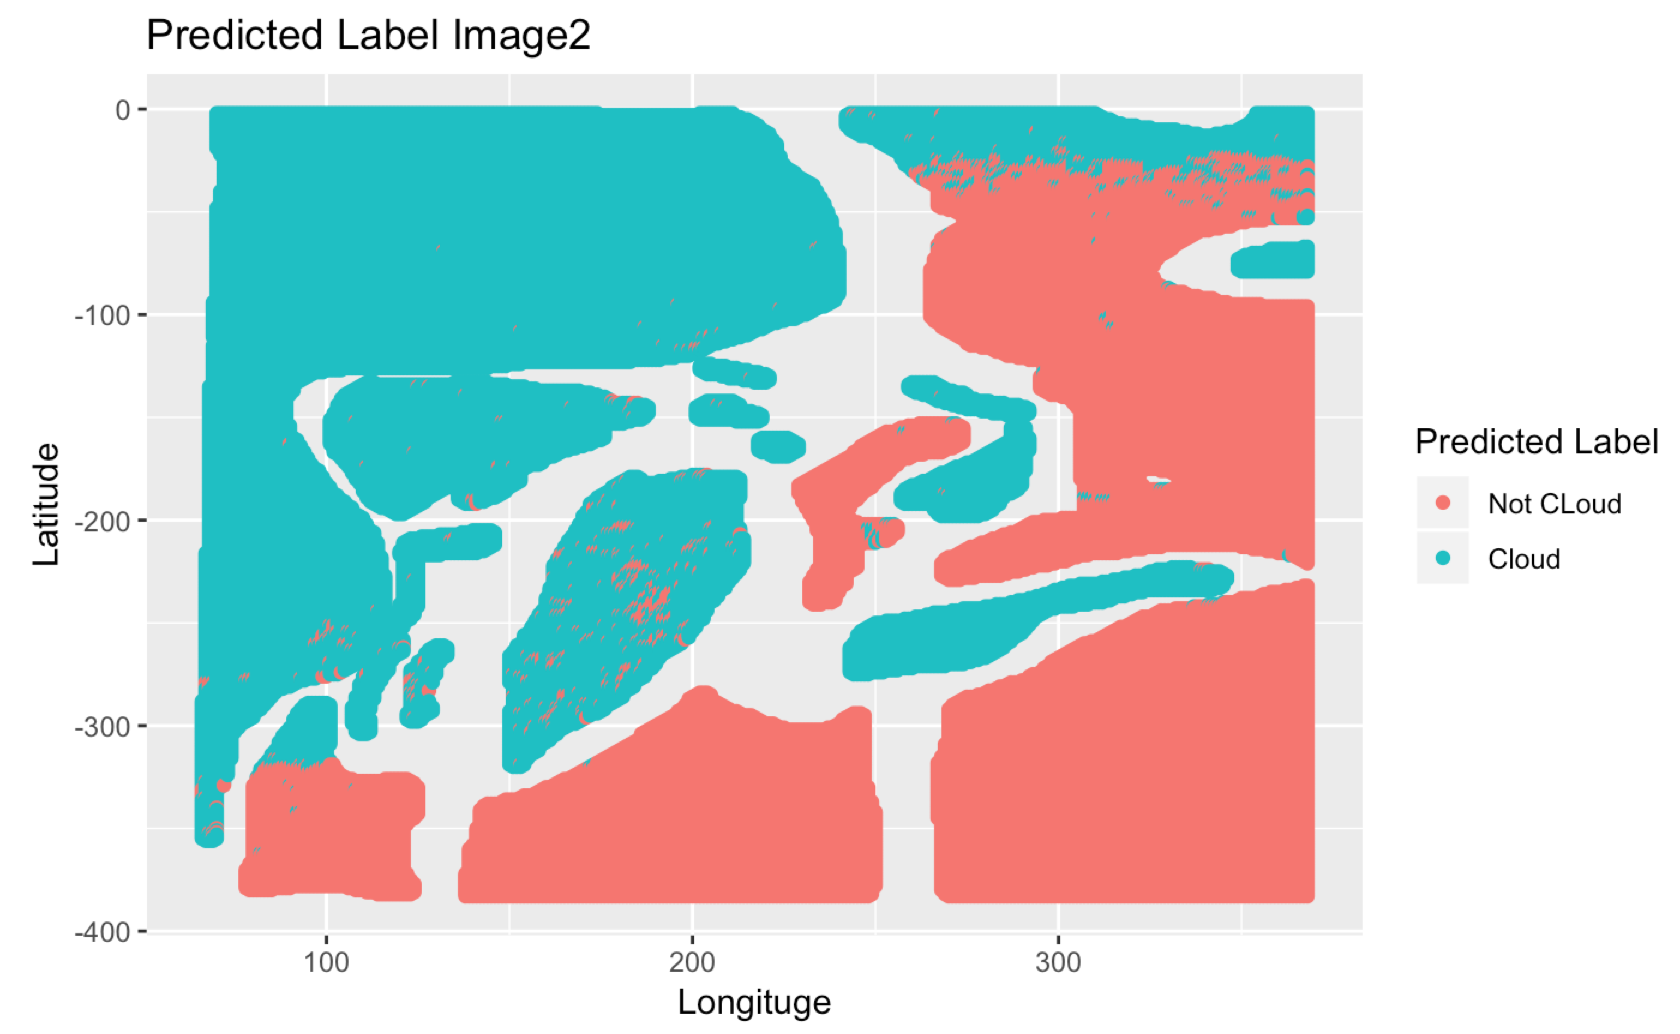
\includegraphics[width = 6cm]{4(b)8}
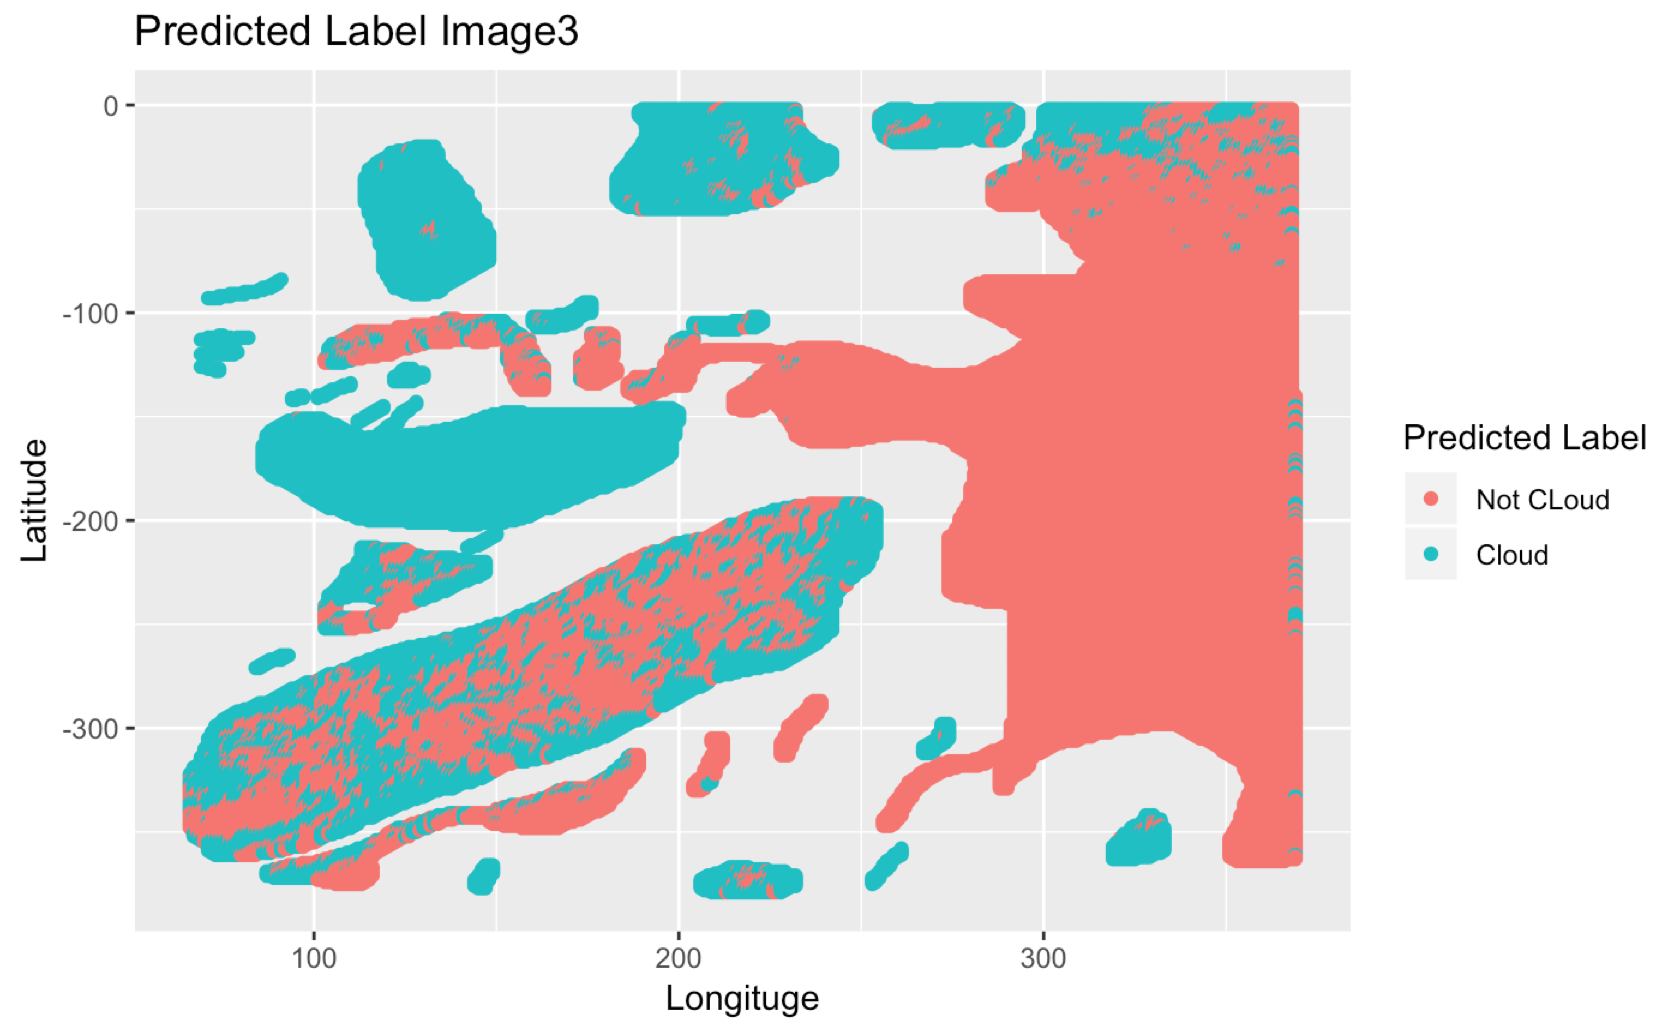
\includegraphics[width = 6cm]{4(b)9}

Comparing these three scatterplots with those in Part1b, we notice that there are several inconsistencies in our plots. The inconsistencies imply the misclassified data points. 

We notice that the data at the boundary of clouded and cloud-free pixels are often misclassified. More importantly, we realize that there are several small blocks that are entirely misclassified. For example, in the first image, the small patch between the upper left two larger patches are classified as cloud while they should have been marked as cloud-free. This is probably because our model is not expressive enough to sperate out the rapid change. In image2, we have significantly fewer misclassified data points. This again verifies that our model is underfitting for image1. The same explanation can also be applied to the third image.


\vspace{0.3cm}
\mbox{}\\
\textbf{c. Better Classifier}

Based on the analysis in the previous two sections, we come up with two ways to improve our classifier.
First, as we mentioned above, the three features selected are not expressive enough to train our model. We decide to add a new feature to train our QDA. Recall the PCA figures we plotted in the second part. Among the rest of the five raw features, DF stands out as the best. Therefore, we add DF as a new feature and train our QDA classification model again on our training data. The final accuracy on test data arises from 0.98930 to 0.99762, which is better than the original QDA model. For future data without expert label, we believe our data can work well because our average accuracy over 8 folds cross validation and test accuracy are quite high. Moreover, QDA won't take that much time to train and predict as other classification methods like svm and knn.

Secondly, QDA requires that the data should be Gaussian distribution, but we cannot ensure that the future data are strictly meet this requirement. Therefore, we also tried Random Forest to train our data. Since we don't have a large number features, Random Forest is suitable in our case.

We first run our model using original three features on training data and get a 0.99418 accuracy on test data.

\vspace{0.3cm}
\mbox{}\\
\textbf{d. Changes after modification of splitting method}

The results change after we use splitting method 1.

\mbox{}\\
Mean and Covariance matrix for design matrix classified as cloud using splitting method 1

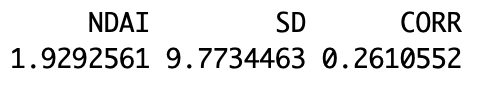
\includegraphics[width = 7.5cm]{4(d)1}
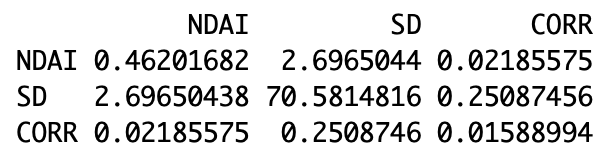
\includegraphics[width = 7.5cm]{4(d)2}

\mbox{}\\
Mean and Covariance matrix for design matrix classified as cloud-free using splitting method 1

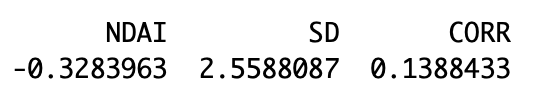
\includegraphics[width = 7.5cm]{4(d)3}
\includegraphics[width = 7.5cm]{4(d)4}

The mean and covariance are 

\includegraphics[width = 7.5cm]{4(d)ndai1}
\includegraphics[width = 7.5cm]{4(d)ndai2}

\includegraphics[width = 7.5cm]{4(d)sd1}
\includegraphics[width = 7.5cm]{4(d)sd2}

\includegraphics[width = 7.5cm]{4(d)corr1}
\includegraphics[width = 7.5cm]{4(d)corr2}

The box plots above show that 

\includegraphics[width = 6cm]{4(d)image1}
\includegraphics[width = 6cm]{4(d)image2}
\includegraphics[width = 6cm]{4(d)image3}


\end{document}
